
% XXX- discuss GtkBin; which widgets have a window, which do not --image and label do not, and we mightwant them too,
%   modify_bg() only affects widgets that have an associated gtk.gdk.Window.
% > Widgets that do not have an associated window include .... gtk.Arrow,
% > gtk.Bin, gtk.Box, gtk.Button, gtk.CheckButton, gtk.Fixed , gtk.Image ,
% > gtk.Label , gtk.MenuItem , gtk.Notebook , gtk.Paned , gtk.RadioButton ,
% > gtk.Range , gtk.ScrolledWindow , gtk.Separator , gtk.Table , gtk.Toolbar ,
% > gtk.AspectFrame , gtk.Frame , gtk.VBox , gtk.HBox , gtk.VSeparator ,
% > gtk.HSeparator . These widgets can be added to a gtk.EventBox to overcome
% > this limitation.




%% RGtk2 chapter
\chapter{RGtk2: Overview}
%%\section{Introduction}
\label{sec:RGtk2-Introduction}
%% intorduction

%% Technical, but short beginning

As the name implies, the \pkg{RGtk2} package is an interface, or
binding, between \R\/ and \GTK, a mature, cross-platform GUI
toolkit. The letters \emph{GTK} stand for the \emph{GIMP ToolKit},
with the word \emph{GIMP} recording the origin of the library as part
of the GNU Image Manipulation Program. \pkg{GTK+} provides the same
widgets on every platform, though it can be customized to emulate
platform-specific look and feel. The library is written in
\proglang{C}, which facilitates access from languages like
\proglang{R} that are also implemented in \proglang{C}. \pkg{GTK+} is
licensed under the \textit{Lesser GNU Public License} (LGPL), while
\pkg{RGtk2} is under the \textit{GNU Public License} (GPL).
The package is available from the Comprehensive \proglang{R} Archive
Network (CRAN) at \url{http://CRAN.R-project.org/package=RGtk2}.

The name \pkg{RGtk2} also implies that there exists a package named
\pkg{RGtk}, which is indeed the case. The original \pkg{RGtk} is bound
to the previous generation of \pkg{GTK+}, version 1.2. \pkg{RGtk2} is
based on \pkg{GTK+ 2.0}, the current generation. This book covers
\pkg{RGtk2} specifically, although many of the fundamental features of
\pkg{RGtk2} are inherited from \pkg{RGtk}. 

\pkg{RGtk2} provides virtually all of the functionality in \GTK\/ to
the \R\/ programmer. In addition, \pkg{RGtk2} interfaces with several
other libraries in the \GTK\/ stack: Pango for font rendering; Cairo
for vector graphics; GdkPixbuf for image manipulation; GIO for
synchronous and asynchronous input/output for files and network
resources; ATK for accessible interfaces; and GDK, an abstraction over
the native windowing system, supporting either X11 or Windows. These
libraries are multi-platform and extensive and have been used for many
major projects, such as the Linux versions of Firefox and Open Office.

The API of each of these libraries is mapped to \R\/ in a way that is
consistent with \R\/ conventions and familiar to the \R\/
user. Much of the \pkg{RGtk2} API consists of autogenerated \R\/
functions that call into one of the underlying libraries. For
example, the \R\/ function \function{gtkContainerAdd} eventually calls
the C function \code{gtk\_container\_add}. The naming convention is
that the C name has its underscores removed and each following letter
capitalized (camelback style).

The full API for \GTK\/ is quite large, and complete documentation of
it is beyond our scope. However, the \GTK\/ documentation is
algorithmically converted into the \R\/ help format during the
generation of \pkg{RGtk2}. This conveniently allows the programmer to
refer to the appropriate documentation within an \R\/ session, without
having to consult a web page, such as
\url{http://library.gnome.org/devel/gtk/stable/}, which lists the
\proglang{C} API of the stable version of \GTK.

In this chapter, we give an overview of how \pkg{RGtk2} maps the
\GTK\/ API, including its classes, constructors, methods, properties,
signals and enumerations, to an \R-level API that is relatively
familiar to, and convenient for, an \R\/ user. 
% A simple GUI will be
% gradually constructed to demonstrate the API.

%%% ------- OOP --------------

\section{Synopsis of the \pkg{RGtk2} API}

Constructing a GUI with \pkg{RGtk2} generally proceeds by constructing
a widget and then configuring it by calling methods and setting
properties. Handlers are connected to signals, and the widget is
combined with other widgets to form the GUI. For example:
\begin{Schunk}
\begin{Sinput}
 button <- gtkButton("Click Me")
 button['image'] <- gtkImage(stock = "gtk-apply", size = "button")
 gSignalConnect(button, "clicked", function(x) message("Hello World!"))
 window <- gtkWindow(show = FALSE)
 window$add(button)
 window$showAll()
\end{Sinput}
\end{Schunk}
% 
Once one understands the syntax and themes of the above example, it is
only a matter of reading through the proceeding chapters and the
documentation to discover all of the widgets and their features. The
rest of this chapter will explain these basic components of the API.

\section{Objects and Classes}

In any toolkit, all widget types have functionality in common. For
example, they are all drawn on the screen in a consistent style. They
can be hidden and shown again. To formalize this relationship and to
simplify implementation by sharing code between widgets, \pkg{GTK+},
like many other toolkits, defines an inheritance hierarchy for its
widget types. In the parlance of object-oriented programming, each
type is represented by a \textit{class}.

For specifying the hierarchy, \pkg{GTK+} relies on \pkg{GObject}, a
\proglang{C} library that implements a class-based, single-inheritance
object-oriented system. A \pkg{GObject} class encapsulates behaviors
that all instances of the class share. Every class has at most one
parent through which it inherits the behaviors of its ancestors. A
subclass can override some specific inherited behaviors. The interface
defined by a class consists of constructors, methods, properties,
and signals. 

The type system supports reflection, so we can, for example, obtain a
list of the ancestors for a given class:
\begin{Schunk}
\begin{Sinput}
 gTypeGetAncestors("GtkWidget")
\end{Sinput}
\begin{Soutput}
[1] "GtkWidget"         "GtkObject"         "GInitiallyUnowned"
[4] "GObject"          
\end{Soutput}
\end{Schunk}
%
For those familiar with object-oriented programming in R, the returned
character vector could be interpreted as it were a class attribute on
an S3 object.

Single inheritance can be restrictive when a class performs multiple
roles in a program. To circumvent this, \pkg{GTK+} adopts the popular
concept of the \textit{interface}, which is essentially a contract
that specifies which methods, properties and signals a class must
implement. As with languages like Java and \proglang{C\#}, a class can
\textit{implement} multiple interfaces, and an interface can be
composed of other interfaces. An interface allows the programmer to
treat all instances of implementing classes in a similar way. However,
unlike class inheritance, the implementation of the methods,
properties and signals is not shared. For example, we list the
interfaces implemented by \class{GtkWidget}:
\begin{Schunk}
\begin{Sinput}
 gTypeGetInterfaces("GtkWidget")
\end{Sinput}
\begin{Soutput}
[1] "GtkBuildable"        "AtkImplementorIface"
\end{Soutput}
\end{Schunk}

We explain the constructors, methods, properties and signals of
classes and interfaces in the following sections and demonstrate them
in the construction of a simple ``Hello World'' GUI, shown in
Figure~\ref{fig:hello-world}. A more detailed and technical
explanation of \pkg{GObject} is available in
Section~\ref{sec:gobject-primer}.

\begin{figure}[h!tbp]
  \begin{center}
    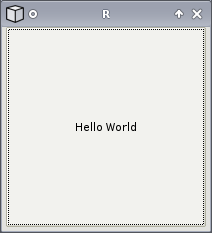
\includegraphics[width=2in]{hello-world.png}
    \caption{\label{fig:hello-world}``Hello World'' in GTK+. 
      A window containing a single button displaying a label with the text
      \code{Hello World}.}
  \end{center}
\end{figure}

\section{Constructors}

The next few sections will contribute to a unifying example that
displays a button in a window. When clicked, the button will print a
message to the R console. The first step in our example is to create a
top-level window to contain our GUI.  Creating an instance of a GTK\/
widget requires calling a single \R\/ function, known as a
constructor. Following \R\/ conventions, the constructor for a class
has the same name as the class, except the first character is
lowercase. The following statement constructs an instance of the
\code{GtkWindow} class:
\begin{Schunk}
\begin{Sinput}
 window <- gtkWindow("toplevel", show = FALSE)
\end{Sinput}
\end{Schunk}
%
The first argument to the constructor for \code{GtkWindow} instructs
the window manager to treat the window as top-level.  The \code{show}
argument is the last argument for every widget constructor. It
indicates whether the widget should be made visible immediately after
construction.  The default value of \code{show} is \code{TRUE}. In
this case we want to defer showing the window until after we finish
constructing our simple GUI.

At the \GTK\/ level, a class usually has multiple constructors, each
implemented as a separate C function. In \pkg{RGtk2}, the names of
these functions all end with \code{New}. The ``meta'' constructor
\function{gtkWindow}, called above, automatically delegates to one of
the low-level constructors, based on the provided arguments.
We prefer these shorter, more flexible constructors, such as
\function{gtkWindow} or \function{gtkButton}, but note their
documentation is provided by the \R\/ package author and is in
addition to the formal API. These constructors can take many
arguments, and only some subsets of the arguments may be specified at
once. For example, this call
\begin{Schunk}
\begin{Sinput}
 gtkImage(stock = "gtk-apply", size = "button")
\end{Sinput}
\end{Schunk}
% 
uses only two arguments, \argument{stock}{gtkImage} and
\argument{size}{gtkImage}, which always must be specified
together. The entire signature is more complex:
\begin{Schunk}
\begin{Sinput}
 args(gtkImage)
\end{Sinput}
\begin{Soutput}
function (size, mask = NULL, pixmap = NULL, image = NULL, filename, 
    pixbuf = NULL, stock.id, icon.set, animation, icon, show = TRUE) 
NULL
\end{Soutput}
\end{Schunk}

A \GTK\/ object created by the \R\/ user has an \R-level object as its
proxy. Thus, \code{window} is a reference to a \class{GtkWindow}
instance. A reference object will not be copied before
modification. This is different from the behavior of most \R\/
objects. For example, calling \function{abs} on a numeric vector does
not change the value assigned to the original symbol:
\begin{Schunk}
\begin{Sinput}
 a <- -1
 abs(a)
\end{Sinput}
\begin{Soutput}
[1] 1
\end{Soutput}
\begin{Sinput}
 a
\end{Sinput}
\begin{Soutput}
[1] -1
\end{Soutput}
\end{Schunk}
% 
Setting the text label on our button, however, will change the
original value:
\begin{Schunk}
\begin{Sinput}
 gtkButtonSetLabel(button, "New text")
 gtkButtonGetLabel(button)
\end{Sinput}
\begin{Soutput}
[1] "New text"
\end{Soutput}
\end{Schunk}
% 
If this widget were displayed on the screen, the label would also be
updated.

The class hierarchy of an object is represented by the
\code{class} attribute. One interprets the attribute according to S3
conventions, so that the class names are in order from most to least
derived:
\begin{Schunk}
\begin{Sinput}
 class(window)
\end{Sinput}
\begin{Soutput}
[1] "GtkWindow"         "GtkBin"            "GtkContainer"     
[4] "GtkWidget"         "GtkObject"         "GInitiallyUnowned"
[7] "GObject"           "RGtkObject"       
\end{Soutput}
\end{Schunk}
%
We find that the \class{GtkWindow} class inherits methods,
properties, and signals from the \class{GtkBin}, \class{GtkContainer},
\class{GtkWidget}, \class{GtkObject}, \class{GInitiallyUnowned}, and
\class{GObject} classes. Every type of \pkg{GTK+} widget inherits from
the base \code{GtkWidget} class, which implements the general
characteristics shared by all widget classes, e.g., properties storing
the location and background color; methods for hiding, showing and
painting the widget. We can also query \code{window} for the
interfaces it implements:
\begin{Schunk}
\begin{Sinput}
 interface(window)
\end{Sinput}
\begin{Soutput}
[1] "GtkBuildable"        "AtkImplementorIface"
\end{Soutput}
\end{Schunk}

When the underlying \GTK\/ object is destroyed, i.e., deleted
from memory, the class of the proxy object is set to \class{<invalid>},
indicating that it can no longer be manipulated.

\section{Methods}

The next steps in our example are to create a ``Hello World'' button
and to place the button in the window that we have already
created. This depends on an understanding of how of one
programmatically manipulates widgets by invoking methods.  Methods are
functions that take an instance of their class as the first argument
and instruct the widget to perform an action.

Although class information is stored in the style of S3, \pkg{RGtk2}
introduces its own mechanism for method dispatch.  The call
\code{obj\$method(...)}  resolves to a function call
\code{f(obj,...)}. The function is found by looking for any function
that matches the pattern \emph{classNameMethodName}, the concatenation
of one of the names from \code{class(obj)} or \code{interface(obj)}
with the method name. The search begins with the interfaces and
proceeds through each character vector in order.

For instance, if \code{win} is a \function{gtkWindow} instance, then
to resolve the call \code{win\$add(widget)} \pkg{RGtk2} considers
\function{gtkBuildableAdd}, \function{atkImplementorIfaceAdd},
\function{gtkWindowAdd}, \function{gtkBinAdd} and finally finds
\function{gtkContainerAdd}, which is called as
\code{gtkContainerAdd(win, widget)}. The \method{\$}{GObject} method
for \pkg{RGtk2} objects does the work.

We take advantage of this convenience when we add the ``Hello World''
button to our window and set its size:
\begin{Schunk}
\begin{Sinput}
 button <- gtkButton("Hello World")
 window$add(button)
 window$setDefaultSize(200, 200)
\end{Sinput}
\end{Schunk}
%
The above code calls the \function{gtkContainerAdd} and
\function{gtkWindowSetDefaultSize} functions with less typing and less
demands on the memory of the user.

Understanding this mechanism allows us to add to the \pkg{RGtk2}
API. For instance, we can add to the button API with
\begin{Schunk}
\begin{Sinput}
 gtkButtonSayHello <- function(obj, target) 
   obj$setLabel(paste("Hello", target))
 button$sayHello("World")
 button$getLabel()
\end{Sinput}
\begin{Soutput}
[1] "Hello World"
\end{Soutput}
\end{Schunk}

%% common methods
Some common methods are inherited by most widgets, as they are defined
in the base \class{GtkWidget} class. These include the methods 
\method{show}{GtkWidget} to specify that the widget should be drawn;
\method{hide}{GtkWidget} to hide the widget until specified;
\method{destroy}{GtkWidget} to destroy a widget and clear up any
references to it; \method{getParent}{gtkWidget} to find the parent
container of the widget; \method{modifyBg}{GtkWidget} to modify the
background color of a widget; and \method{modifyFg}{GtkWidget} to
modify the foreground color.


\section{Properties}


%% --------- Properties ------------
The \GTK\/ API uses properties to store object state. Properties are
similar to R attributes and even more so to S4 slots. They are
inherited, typed, self-describing and encapsulated, so that an object
can intercept access to the underlying data. A list of properties
definitions belonging to the widget is returned by its
\method{getPropInfo}{GObject} method. Calling \function{names} on the
object returns the property names. Auto-completion of property names
is gained as a side effect.  For the button just defined, we can see
the first eight properties listed with:
\begin{Schunk}
\begin{Sinput}
 head(names(button), n=8)                 # or b$getPropInfo()
\end{Sinput}
\begin{Soutput}
[1] "related-action"        "use-action-appearance"
[3] "user-data"             "name"                 
[5] "parent"                "width-request"        
[7] "height-request"        "visible"              
\end{Soutput}
\end{Schunk}

Some common properties are: \code{parent}, to store the parent widget
(if any); \code{user-data}, which allows one to store arbitrary data
with the widget; and \code{sensitive}, to control whether a widget can
receive user events. 

There are a few different ways to access these properties. The methods
\method{get}{GObject} and \method{set}{GObject} get and set properties
of a widget, respectively. The set funtion treats the argument names
as the property names, and setting multiple properties at once is
supported. Here we add an icon to the top-left corner of our window
and set the title:
\begin{Schunk}
\begin{Sinput}
 image <- gdkPixbuf(filename = imagefile("rgtk-logo.gif"))[[1]]
 window$set(icon = image, title = "Hello World 1.0")
\end{Sinput}
\end{Schunk}

Additionally, most user-accessible properties have specific \code{get} and
\code{set} methods defined for them. For example, to set the title of
the window, we could have used the \method{setTitle}{GtkWindow} method
and verified the change with \method{getTitle}{GtkWindow}.
\begin{Schunk}
\begin{Sinput}
 window$setTitle("Hello World 1.0")
 window$getTitle()
\end{Sinput}
\begin{Soutput}
[1] "Hello World 1.0"
\end{Soutput}
\end{Schunk}

\pkg{RGtk2} provides the convenient and familiar \code{[} and
\code{[$<$-} methods to get and access the properties. In our example,
we might check the window to ensure that it is not yet visible:
\begin{Schunk}
\begin{Sinput}
 window["visible"]
\end{Sinput}
\begin{Soutput}
[1] FALSE
\end{Soutput}
\end{Schunk}
Finally, we can make our window visible by setting the ``visible'' property,
although calling \function{gtkWidgetShow} is more conventional:
\begin{Schunk}
\begin{Sinput}
 window["visible"] <- TRUE 
 window$show() # same effect
\end{Sinput}
\end{Schunk}

For ease of referencing the appropriate help pages, we tend to use the
full method name in the examples, although at times the move \R-like
vector notation will be used for commonly accessed properties.

%%% ------ Signals ----------

\section{Events and signals}

In \pkg{RGtk2}, a user action, such as a mouse click, key press or
drag and drop motion triggers the widget to emit a corresponding
signal.  A GUI can be made interactive by specifying a callback
function to be invoked upon the emission of a particular signal.

The signals provided by a class or interface are returned by the
function \function{gTypeGetSignals}. For example
\begin{Schunk}
\begin{Sinput}
 names(gTypeGetSignals("GtkButton"))
\end{Sinput}
\begin{Soutput}
[1] "pressed"  "released" "clicked"  "enter"    "leave"   
[6] "activate"
\end{Soutput}
\end{Schunk}
shows the ``clicked'' signal in addition to others. Note that this
only lists the signals provided directly by the \class{GtkButton}. To
list all inherited signals, we need to loop over the hierarchy, but it
is not common to do this in practice, as the documentation includes
information on the signals.

The \function{gSignalConnect} function adds a callback to a widget's
signal. Its signature is
\begin{Schunk}
\begin{Sinput}
 args(gSignalConnect)
\end{Sinput}
\begin{Soutput}
function (obj, signal, f, data = NULL, after = FALSE, user.data.first = FALSE) 
NULL
\end{Soutput}
\end{Schunk}
%
The basic usage is to call \function{gSignalConnect} to connect a
callback function \argument{f}{gSignalConnect} to the signal named
\argument{signal}{gSignalConnect} belonging to the object
\argument{obj}{gSignalConnect}. The function returns an identifier for
managing the connection. This is not usually necessary but will be
discussed later.

We demonstrate this usage by adding a callback to our ``Hello World''
example, so that ``Hello World'' is printed to the console when the
button is clicked:
\begin{Schunk}
\begin{Sinput}
 gSignalConnect(button, "clicked", 
                function(widget) print("Hello world!"))
\end{Sinput}
\end{Schunk}
%

The \argument{data}{gSignalConnect} argument allows arbitrary data to
be passed to the callback.  The
\argument{user.data.first}{gSignalConnect} argument specifies if the
\argument{data}{gSignalConnect} argument should be the first argument
to the callback or (the default) the last.

The \argument{after}{gSignalConnect} argument is a logical value
indicating if the callback should be called after the default handler
(see \command{?gSignalConnect}).

%% the callback
The signature for the callback varies for each signal. Unless
\code{user.data.first} is \code{TRUE}, the first argument is the
widget. Other arguments are possible depending on the signal type. For
window events, the second argument is a \class{GdkEvent} type, which
can carry with it extra information about the event that occurred. The
\GTK\/ API lists the signature of each signal.

Is important to note that the widget, and possibly other arguments,
are references, so their manipulation has side effects outside of the
callback. This is obviously a critical feature, but it is one that
may be surprising to the \R\/ user.

\begin{Schunk}
\begin{Sinput}
 w <- gtkWindow(); w['title'] <- "test signals"
 x <- 1; 
 b <- gtkButton("click me"); w$add(b)
 ID <- gSignalConnect(b, signal = "clicked", 
                      f = function(widget) {
                        widget$setData("x", 2)
                        x <- 2
                        return(TRUE)
                      })
\end{Sinput}
\end{Schunk}
Then after clicking, we would have

\begin{Schunk}
\begin{Sinput}
 cat(x, b$getData("x"), "\n") # 1 and 2
\end{Sinput}
\begin{Soutput}
1 2 
\end{Soutput}
\end{Schunk}

Callbacks for signals emitted by window manager events are expected to
return a logical value. Failure to do so can cause errors to be
raised. A return value of \code{TRUE} indicates that no further
callbacks should be called, whereas \code{FALSE} indicates that the
next callback should be called. In other words, the return value
indicates whether the handler has consumed the event. In the following
example, only the first two callbacks are executed when the user
clicks the button:
\begin{Schunk}
\begin{Sinput}
 b <- gtkButton("click")
 w <- gtkWindow()
 w$add(b)
 id1 <- gSignalConnect(b, "button-press-event", 
 function(b, event, data) {
   print("hi"); return(FALSE)
 })
 id2 <- gSignalConnect(b, "button-press-event", 
 function(b, event, data) {
   print("and"); return(TRUE)
 })
 id3 <- gSignalConnect(b, "button-press-event", 
 function(b, event, data) {
   print("bye"); return(TRUE)
 })
\end{Sinput}
\end{Schunk}

%% multiple callbacks; remove; block
Multiple callbacks can be assigned to each signal. They will be
processed in the order they were bound to the signal.  The
\function{gSignalConnect} function returns an ID that can be used to
disconnect a handler, if desired, using
\function{gSignalHandlerDisconnect}. To temporarily block a handler,
call \function{gSignalHandlerBlock} and then
\function{gSignalHandlerUnblock} to unblock. The man page for
\function{gSignalConnect} gives the details on this.

%%% ------ constants --------

\section{Enumerated types and flags}

At the beginning of our example, we constructed the window thusly: 
\begin{Schunk}
\begin{Sinput}
 window <- gtkWindow("toplevel", show = FALSE)
\end{Sinput}
\end{Schunk}
%
The first parameter indicates the window type. The set of possible
window types is specified by what in C is known as an
\textit{enumeration}. A value from an enumeration can be thought of as a
length one factor in \R. The possible values defined by the
enumeration are analogous to the factor levels.  Since enumerations
are foreign to R, \pkg{RGtk2} accepts string
representations of enumeration values, like \code{"toplevel"}. 

For every \GTK\/ enumeration, \pkg{RGtk2} provides an R
vector that maps the nicknames to the underlying numeric values.  In
the above case, the vector is named \class{GtkWindowType}.
\begin{Schunk}
\begin{Sinput}
 GtkWindowType
\end{Sinput}
\begin{Soutput}
An enumeration with values:
toplevel    popup 
       0        1 
\end{Soutput}
\end{Schunk}
%
The names of the vector indicate the allowed nickname for each value
of the enumeration. It is rarely necessary to explicitly use the
enumeration vectors; specifying the nickname will work in most cases,
including all method invocations, and is preferable as it is easier
for human readers to comprehend.

Flags are an extension of enumerations, where the value of each member
is a unique power of two, so that the values can be combined
unambiguously. An example of a flag enumeration is
\class{GtkWidgetFlags}.
\begin{Schunk}
\begin{Sinput}
 GtkWidgetFlags
\end{Sinput}
\begin{Soutput}
A flag enumeration with values:
        toplevel        no-window         realized 
              16               32               64 
          mapped          visible        sensitive 
             128              256              512 
parent-sensitive        can-focus        has-focus 
            1024             2048             4096 
     can-default      has-default         has-grab 
            8192            16384            32768 
        rc-style  composite-child      no-reparent 
           16384           131072           262144 
   app-paintable receives-default  double-buffered 
          524288          1048576          2097152 
     no-show-all 
         4194304 
\end{Soutput}
\end{Schunk}
%
\class{GtkWidgetFlags} represents the possible flags that can be set
on a widget. We can retrieve the flags currently set on our window:



\begin{Schunk}
\begin{Sinput}
 window$flags()
\end{Sinput}
\end{Schunk}
\begin{Soutput}
GtkWidgetFlags: toplevel, realized, mapped, visible, 
         sensitive, parent-sensitive, double-buffered
\end{Soutput}
%
Flag values can be combined using 
%% JV: \function{\\|}, 
\verb+|+
the bitwise
\textit{OR}. The \function{\&} function, the bitwise \textit{AND},
allows one to check whether a value belongs to a combination. For
example, we could check whether our window is top-level:
\begin{Schunk}
\begin{Sinput}
 (window$flags() & GtkWidgetFlags["toplevel"]) > 0
\end{Sinput}
\begin{Soutput}
[1] TRUE
\end{Soutput}
\end{Schunk}

%% --------- Event Loop

\section{The event loop}

\pkg{RGtk2} integrates the \GTK\/ and \R\/ event loops by treating the
\R\/ loop as the master and iterating the \GTK\/ event loop whenever R
is idle.  During a long calculation, the GUI can seem unresponsive. To
avoid this, the following construct should be inserted into the long
running algorithm in order to ensure that \GTK\/ events are
periodically processed:
\begin{Schunk}
\begin{Sinput}
 while(gtkEventsPending()) 
   gtkMainIteration()
\end{Sinput}
\end{Schunk}
This is often useful, for example, to update a progress bar.

If one runs an \pkg{RGtk2} script non-interactively, such as by
assigning an icon to launch a GUI under Windows, R will exit after
the script is finished and the GUI will disappear just after it
appears. To work around this, call the function \function{gtkMain} to
run the main loop until the function \function{gtkMainQuit} is
called. Since there is no interactive session, \function{gtkMainQuit}
should be called through some event handler.

%% FIXME: here or in the appendix?
\section{Importing a GUI from Glade}
\label{sec:gtk-glade}

%% Using Glade

This book focuses almost entirely on the direct programmatic
construction of GUIs. Some developers prefer visually constructing a
GUI by pointing, clicking and dragging in another GUI, which one might
call a GUI builder, a type of RAD (Rapid Application Development)
tool. \pkg{Glade} is the primary GUI builder for \GTK/ and
exports an interface as XML that is loadable by \class{GtkBuilder}. It
is freely available for all major platforms from
\url{http://glade.gnome.org/}. Documentation is also at that
location. 

We will assume that the reader has saved an interface as a
\class{GtkBuilder} XML file named \code{buildable.xml} and is ready to
load it with \pkg{RGtk2}:
%% JV XXX no constructor? (un eval=FALSE the next 3)
\begin{Schunk}
\begin{Sinput}
 g <- gtkBuildableNew()
 g$addFromFile("buildable.xml")
\end{Sinput}
\end{Schunk}

The \method{getObject}{gtkBuilder} extracts a widget by its ID, which
is specified by the user through \pkg{Glade}. It normally
suffices to load the top-level widget, named \code{dialog1} in this
example, and show it:
\begin{Schunk}
\begin{Sinput}
 d <- g$getObject("dialog1")
 d$showAll()
\end{Sinput}
\end{Schunk}

In order to add behaviors to the GUI, we need to register R functions
as signal handlers. In \pkg{Glade}, the user should specify the
name of an R function as a handler for some signal. \pkg{RGtk2}
extends \class{GtkBuilder} to look up the functions and connect them
to the appropriate signals. Let us assume that the user has named the
\function{ok\_button\_clicked} function as the handler for the
\signal{clicked} signal on a \class{GtkButton}. The
\method{connectSignals}{GtkBuilder} method will establish that
connection and any others in the interface:
\begin{Schunk}
\begin{Sinput}
 ok_button_clicked <- function(w, userData) {
   print("hello world")
 }
 g$connectSignals()
\end{Sinput}
\end{Schunk}
% 
The GUI should now be ready for use.

%% MOVEME: seems like integration between gWidgets and native toolkits
%% belongs in the gWidgets chapters. Otherwise, each toolkit chapter
%% needs to say the same thing. Better to have it in one place.

% \section{RGtk2 and gWidgetsRGtk2}
% \label{sec:RGtk2:gWidgetsRGtk2}


% The widgets described above, are also available through
% \pkg{gWidgetsRGtk2}. The two packages can be used together, for the
% most part. The \code{add} method of \pkg{gWidgetsRGtk2} can be used to
% add an \pkg{RGtk2} widget to a \code{gWidgetsRGtk2}
% container. Whereas, the \code{getToolkitWidget} method will (usually)
% return the \pkg{RGtk2} component to use within \pkg{RGtk2}.

%% Views example in next chapter?

\chapter{RGtk2: Windows, Containers, and Dialogs}
\label{sec:top-level-windows}
%% JV: 1/14/11: I moved this around following your comments after top
%% level windows: dialogs are now after box containers (as they are
%% needed for the example); discussion on other containers
%% follows. Then I moved the basic controls into a separate chapter,
%% as this one got rather long.




%% JV: 1/27/11 This intro para. needed a rewrte 
% This section covers some of the basic widgets and containers of
% \GTK. We begin with a discussion of top level containers and box
% containers. Then we describe many of the basic controls, and
% conclude with the mention of a few special-case containers.


This chapter covers top-level windows, dialogs and the container
objects provided by \GTK.

\section{Top-level windows}
\label{sec:RGtk2:gtkWindow}

%% constructor Show/Hide
As we saw in our ``Hello World'' example, top-level windows are
constructed by the \constructor{gtkWindow} constructor. This function
has arguments \code{type} to specify the type of window to create. The
default is a top-level window, which we will always use, as the
alternative is for ``popups'' which are meant for internal use, e.g.,
for implementing menus. The second argument is \code{show}, which by
default is \code{TRUE}, indicating that the window should be shown. If
set to \code{FALSE}, the window, like other widgets, can later be
shown by calling its \method{show}{gtkWidget} method. The
\method{showAll}{gtkWidget} method will also show any child
components. These can be reversed with \method{hide}{gtkWidget} and
\method{hideAll}{gtkWidget}.

%% title
As with all objects, windows have several properties. The window title
is stored in the \code{title} property. As usual, this property can be
accessed via the ``get'' and ``set'' methods
\method{getTitle}{gtkWindow} and \method{setTitle}{gtkWindow}, or
using the \function{[} function. To illustrate, the following sets up
a new window with a title.
\begin{Schunk}
\begin{Sinput}
 w <- gtkWindow(show=FALSE)              # use default type
 w$setTitle("Window title")              # set window title
 w['title']                              # or  use getTitle
\end{Sinput}
\begin{Soutput}
[1] "Window title"
\end{Soutput}
\begin{Sinput}
 w$setDefaultSize(250,300)               # 250 wide, 300 high
 w$show()                                # show window
\end{Sinput}
\end{Schunk}

\paragraph{Window size}
The initial size of the window can be set with the
\method{setDefaultSize}{gtkWindow} method, as shown above, which takes a
\argument{width}{gtkWindow} and \argument{height}{gtkWindow} argument
specified in pixels. This specification allows the window to be
resized but must be made before the window is drawn, as the window
then falls under control of the window manager. The
\method{setSizeRequest}{gtkWidget} method will request a minimum size,
which the window manager will usually honor, as long as a maximum
bound is not violated. To fix the size of a window, the
\code{resizable} property may be set to \code{FALSE}.

%% A container
\paragraph{Adding a child component to a window}
A window is a container. \class{GtkWindow} inherits from
\class{GtkBin}, which derives from \class{GtkContainer} and allows
only a single child. As before, this child is added through the
\method{add}{gtkContainer} method. 
We illustrate the basics by adding a simple label to a window.
\begin{Schunk}
\begin{Sinput}
 w <- gtkWindow(show=FALSE); w$setTitle("Hello world")
 l <- gtkLabel("Hello world")
 w$add(l)
\end{Sinput}
\end{Schunk}
%
To display multiple widgets in a
window, one simply needs to add a non-\class{GtkBin} container as the
child widget.

%% delete-event; destroy
\paragraph{Destroying windows}
A window is normally closed by the window manager. Most often, this
occurs in response to the user clicking on a close button in a title
bar.  When the user clicks on the
close button, the window manager requests that the window be deleted,
and the \code{delete-event} signal is emitted. As with any window
manager event, the default handler is overridden if a callback
connected to \code{delete-event} returns \code{TRUE}.  This can be
useful for confirming the intention of the user before closing the
window. For example:
\begin{Schunk}
\begin{Sinput}
 gSignalConnect(w, "delete-event", function(event) {
   gtkMessageDialog(parent=w, flags=0, type="question", buttons=c("yes", "no"),
                    "Are you sure you want to quit?")
   dlg$run() != GtkResponseType["yes"]
 })
\end{Sinput}
\end{Schunk}
%
We describe the use of message dialogs in
Section~\ref{sec:gtk-dialog-message}. The contract of deletion is that
the window should no longer be visible on the screen. It is not
necessary for the actual window object to be removed from memory,
although this is the default behavior. Calling the \code{hideOnDelete}
method configures the window to hide but not destroy itself.

It is also possible to close a window programmatically by calling
its \method{destroy}{gtkWidget} method:
\begin{Schunk}
\begin{Sinput}
 w$destroy()
\end{Sinput}
\end{Schunk}

\paragraph{Transient windows}
New windows may be standalone top-level windows or may be associated
with some other window. For example, a dialog is usually associated
with the primary document window. The
\method{setTransientFor}{gtkWindow} method can be used to specify the
window with which a transient (dialog) window is associated. This
hints to the window manager that the transient window should be kept on
top of its parent. The position relative to the parent window can be
specified with \code{setPostion}, which takes a value from the
\code{GtkWindowPosition} enumeration. Optionally, a dialog can be
set to be destroyed with its parent. For example:
\begin{Schunk}
\begin{Sinput}
 w <- gtkWindow(show=FALSE); w$setTitle("Top level window")
 d <- gtkWindow(show=FALSE); d$setTitle("dialog window")
 d$setTransientFor(w)
 d$setPosition("center-on-parent")
 d$setDestroyWithParent(TRUE)
 w$show()
 d$show()
\end{Sinput}
\end{Schunk}
% 
The above code produces a non-modal dialog window from scratch. Due to
its transient nature, it can hide parts of the top-level window, but,
unlike a modal dialog, it does not prevent that window from receiving
events. \GTK\/ provides a number of convenient high-level dialogs,
discussed in Section~\ref{sec:dialogs}, that support modal operation.

\section{Layout containers}
\label{sec:RGtk2:layout}

Once a top-level window is constructed, it remains to fill the window
with the controls that will constitute our GUI. As these controls are
graphical, they must occupy a specific region on the screen. The
region could be specified explicitly, as a rectangle. However, as a
user interface, a GUI is dynamic and interactive. The size constraints
of widgets will change, and the window will be resized. The programmer
cannot afford to explicitly manage a dynamic layout. Thus, \GTK\/
implements automatic layout in the form of container widgets.

\subsection{Basics}
\label{sec:RGtk2:layout:basics}

In \GTK{}, the widget hierarchy is built when children are added to a
parent container.  In this example, a window is made the parent of a
label: 
\begin{Schunk}
\begin{Sinput}
 w <- gtkWindow(show=FALSE); w$setTitle("Hello world")
 l <- gtkLabel("Hello world")
 w$add(l)
\end{Sinput}
\end{Schunk}

The method \method{getChildren}{GtkContainer} will return the children
of a container as a list. Since in this case the list will be at most
length one, the \method{getChild}{GtkWidget} method may be more
convenient, as it directly returns the only child, if any. For
instance, to retrieve the label text one could do:
\begin{Schunk}
\begin{Sinput}
 w$getChild()['label']
\end{Sinput}
\begin{Soutput}
[1] "Hello world"
\end{Soutput}
\end{Schunk}
%% [[ for container
The \method{[[}{GObject} method 
%% ]]
accesses the child widgets by number, as a convenient wrapper
around the \method{getChildren}{GObject} method:
\begin{Schunk}
\begin{Sinput}
 w[[1]]['label']
\end{Sinput}
\begin{Soutput}
[1] "Hello world"
\end{Soutput}
\end{Schunk}
%
Conversely, the \code{getParent} method for \GTK\/ widgets will
return the parent container of a widget.

Every container supports removing a child with the
\method{remove}{gtkWidget} method. The child can later be re-added.
For instance
\begin{Schunk}
\begin{Sinput}
 w$remove(l)
 w$add(l)
\end{Sinput}
\end{Schunk}
% 
To remove a widget from the screen but not its container, use the
\method{hide}{gtkWidget} method on the widget. The
\method{reparent}{gtkWidget} method is a convenience for moving a
widget between containers that ensures the child is not garbage
collected during the transition.

\subsection{Widget size negotiation}
\label{sec:RGtk2:layout:size}

We have already seen perhaps the simplest automatic layout container,
\class{GtkWindow}, which fills all of its space with its
child. Despite the apparent simplicity, there is a considerable amount
of logic for calculating the size of the widget on the screen. The
child will first inform the parent of its desired natural size. For
example, a label might ask for the dimensions necessary to display all
of its text. The container then decides whether to allocate the
requested size or to allocate more or less than the requested
amount. The child then consumes the allocated space. Consider the
previous example of adding a label to a window:
\begin{Schunk}
\begin{Sinput}
 w <- gtkWindow(); w$setTitle("Hello world")
 l <- gtkLabel("Hello world")
 w$add(l)
\end{Sinput}
\end{Schunk}

%% Oddly this is choking for me
% <<layout-window-show-first>>=
% <<basic-window-label>>
% @
%
The window is shown before the label is added, and the default size is
likely much larger than the space the label needs to display ``Hello
world''. However, as the window size is now controlled by the window
manager, \class{GtkWindow} will not adjust its size. Thus, the label
is allocated more space than it requires.
\begin{Schunk}
\begin{Sinput}
 l$getAllocation()$allocation
\end{Sinput}
\end{Schunk}
% JV: We tighten up the output here:
\begin{Schunk}
\begin{Soutput}
     x      y  width height 
    -1     -1      1      1 
\end{Soutput}
\end{Schunk}
%
If, however, we avoid showing the window until the label is added, the
window will size itself so that the label has its natural size:
\begin{Schunk}
\begin{Sinput}
 w <- gtkWindow(show=FALSE); w$setTitle("Hello world")
 l <- gtkLabel("Hello world")
 w$add(l)
 w$show()
 l$getAllocation()$allocation
\end{Sinput}
\end{Schunk}
\begin{Schunk}
\begin{Soutput}
     x      y  width height 
     0      0     79     18 
\end{Soutput}
\end{Schunk}
%
One might notice that it is not possible to decrease the size of the
window further. This is due to \class{GtkLabel} asserting a minimum
size request that is sufficient to display its text. The
\method{setSizeRequest}{GtkWidget} sets a user-level minimum size 
request for any widget. It is obvious from the method name, however,
that this is still strictly a request. It may not be satisfied, for
example, if the maximum window size constraint of the window manager
is violated. More importantly, setting a minimum size request is
generally discouraged, as it decreases the flexibility of the layout.

Any non-trivial GUI will require a window containing multiple
widgets. Let us consider the case where the child of the window is
itself a container, with multiple children.  Essentially the same
negotiation process occurs between the container and its children (the
grandchildren of the window). The container calculates its size
request based on the requests of its children and communicates it to
the window. The size allocated to the container is then distributed to
the children according to its layout algorithm. This process is the
same for every level in the container hierarchy.

\subsection{Box containers}
\label{sec:RGtk2:layout:box}

The most commonly used multi-child container in \GTK\/ is the box,
\class{GtkBox}, which packs its children as if they were in a
box. Instances of \class{GtkBox} are constructed by \function{gtkHBox}
or \function{gtkVBox}.  These produce horizontal or vertical boxes,
respectively. Each child widget is allocated a cell in the box.  The
cells are arranged in a single column (\class{GtkVBox}) or row
(\class{GtkHBox}). This one dimensional stacking is usually all that a
layout requires. The child widgets can be containers themselves,
allowing for very flexible layouts. For special cases where some
widgets need to span multiple rows or columns and align themselves in
both dimensions, \GTK\/ provides the \class{GtkTable} class, which is
discussed later.  Many of the principles we discuss in this section
also apply to \class{GtkTable}.

Here we will explain and demonstrate the use of \class{GtkHBox}, the
general horizontal box layout container. \class{GtkVBox} can be used
exactly the same way; only the direction of stacking is different.
Figure~\ref{fig:packing} illustrates a sampling of the possible
layouts that are possible with a \class{GtkHBox}.

%% JV: Michael, I don't have this figure and am not sure what to put
%% here. Can you show me the code or a figure? THanks.
%% ML: I put the figure in here, but it's somewhat redundant with your
%% example. Could we adjust your example just to show padding? It
%% seems like we could get rid of the fourth row and add a row where
%% fill and expand are TRUE but padding is 10.
%% JV: We need to tighten this up, but your figure has a much better
%% layout. I'll put the two together as suggested, but keep your
%% frames and numbering. XXX TODO
\begin{figure}[h!tbp]
  \begin{center}
    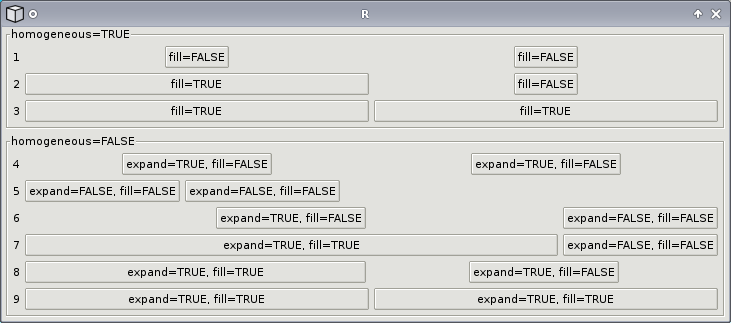
\includegraphics[angle=90, width=.65\textwidth]{packing.png}
    \caption{\label{fig:packing}A screenshot demonstrating the effect
      of packing two buttons into \class{GtkHBox} instances using the
      \method{packStart}{GtkBox} method with different combinations of
      the \argument{expand}{gtkBoxPackStart} and
      \argument{fill}{gtkBoxPackStart} settings.  The effect of the
      \argument{homogeneous}{gtkBoxPackStart} spacing setting on the
      \class{GtkHBox} is also shown.}
  \end{center}
\end{figure}

The code for some of these layouts is presented here. We begin by
creating a \class{GtkHBox} widget. We pass \code{TRUE} for the first
parameter, \argument{homogeneous}{gtkHBox}. This means that the
horizontal allocation of the box will be evenly distributed between
the children.  The second parameter directs the box to leave 5 pixels
of space between each child.  The following code constructs the
\class{GtkHBox}:
\begin{Schunk}
\begin{Sinput}
 box <- gtkHBox(TRUE, 5)
\end{Sinput}
\end{Schunk}
The equal distribution of available space is strictly enforced; the
minimum size requirement of a homogeneous box is set such that the box
always satisfies this assertion, as well as the minimum size
requirements of its children.

The \method{packStart}{GtkBox} and \method{packEnd}{GtkBox} methods pack a
widget into a box against the left and right side (top and
bottom for a \class{GtkVBox}), respectively. For this explanation, we
restrict ourselves to \method{packStart}{GtkBox}, since
\method{packEnd}{GtkBox} works the same except for the
direction. Below, we pack two buttons, \code{button\_a} and
\code{button\_b} against the left side:
\begin{Schunk}
\begin{Sinput}
 button_a <- gtkButton("Button A")
 button_b <- gtkButton("Button B")
 box$packStart(button_a, fill = FALSE)
 box$packStart(button_b, fill = FALSE)
\end{Sinput}
\end{Schunk}
%
First, \code{button\_a} is packed against the left side of the box,
and then we pack \code{button\_b} against the right side of
\code{button\_a}. This results in the first row in
Figure~\ref{fig:packing}. The space distribution is homogeneous, but
making the space available to a child does not mean that the child
will fill it. That depends on the natural size of the child, as well
as the value of the \argument{fill}{gtkBoxPackStart} parameter passed
to \method{packStart}{GtkBox}. In this case,
\argument{fill}{gtkBoxPackStart} is \code{FALSE}, so the extra space
is not filled and the widget is aligned in the center of its
space. When a widget is packed with the
\argument{fill}{gtkBoxPackStart} parameter set to \code{TRUE}, the
widget is resized to consume the available space. This results in
rows~$2$ and $3$ in Figure~\ref{fig:packing}.

In many cases, it is desirable to give children unequal amounts of
available space, as in rows~4--9 in Figure~\ref{fig:packing}. 
To create a heterogeneously spaced \class{GtkHBox}, we pass
\code{FALSE} as the first argument to the constructor, as in the
following code:
\begin{Schunk}
\begin{Sinput}
 box <- gtkHBox(FALSE, 5)
\end{Sinput}
\end{Schunk}

A heterogeneous layout is freed of the restriction that all widgets
must be given the same amount of available space; it only needs to
ensure that each child has enough space to meet its minimum size
requirement. After satisfying this constraint, a box is often left
with extra space. The programmer may control the distribution of this
extra space through the \argument{expand}{gtkBoxPackStart} parameter
to \method{packStart}{GtkBox}.  When a widget is packed with
\argument{expand}{gtkBoxPackStart} set to \code{TRUE}, we will call
the widget an \emph{expanding} widget. All expanding widgets in a box
are given an equal portion of the entirety of the extra space. If no
widgets in a box are expanding, as in row~5 of
Figure~\ref{fig:packing}, the extra space is left undistributed. 

It is common to mix expanding and non-expanding widgets in the same
box.
% FIXME: do we use the mirror dialog example or another one?  For
% example, in the CRAN mirrors dialog, the box first ensures that the
% mirror list and the label above it are given enough space to satisfy
% their minimum requirement. Then, since the mirror list is expanding,
% all of the extra space is made available to it, while the label is
% left only with its minimum requirement (i.e., enough space to show
% its text).
An example is given below, where \code{button\_a} is expanding,
while \code{button\_b} is not:
%
\begin{Schunk}
\begin{Sinput}
 box$packStart(button_a, expand = TRUE, fill = FALSE)
 box$packStart(button_b, expand = FALSE, fill = FALSE)
\end{Sinput}
\end{Schunk}
%
The result is shown in row~6 of Figure~\ref{fig:packing}.  The figure
contains several other permutations of the
\argument{homogeneous}{gtkBoxPackStart},
\argument{expand}{gtkBoxPackStart} and
\argument{fill}{gtkBoxPackStart} settings.

\begin{figure}
  \centering
%%    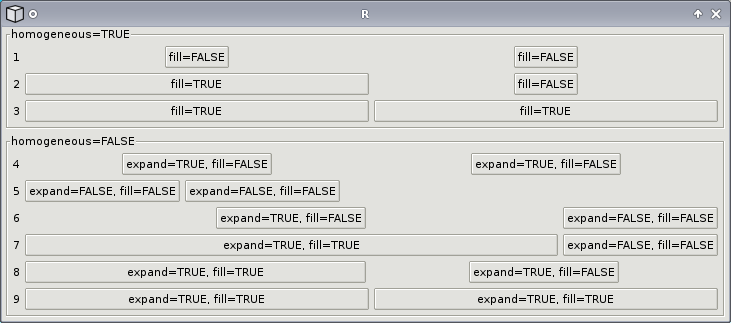
\includegraphics[angle=90, height=.8\textheight, width=.75\textwidth]{packing.png} 
  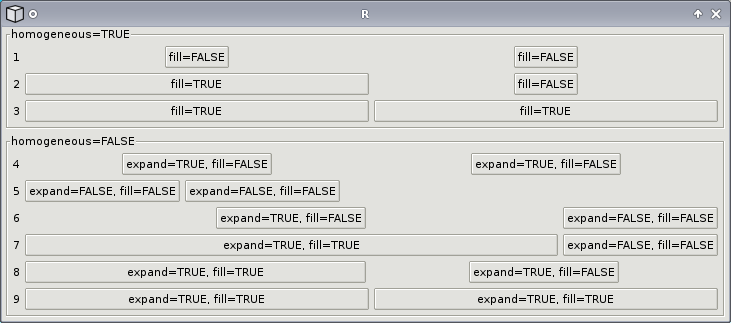
\includegraphics[width=.95\textwidth]{packing.png} 
  \caption{Examples of packing widgets into a box container. The top
    row shows no padding, whereas the 2nd and 3rd illustrate the
    difference between \code{padding} (an amount around each child)
    and \code{spacing} (an amount between each child). The last two
    rows show the effect of \code{fill} when \code{expand=TRUE}. This
    illustration follows one in original \GTK\/ tutorial.}
  \label{fig:RGtk2-pack-start}
\end{figure}

There are several ways to add space around widgets in a box container.
The \argument{spacing}{gtkHBox} argument for the constructors
specifies the amount of space, in pixels, between the cells. This
defaults to zero. The \code{pack} methods have a
\argument{padding}{gtkBoxPackStart} argument, also defaulting to zero,
for specifying the padding in pixels on either side of the child. It
is important to note the difference: \code{spacing} is between
children and the same for every boundary, while the \code{padding} is
specific to a particular child and occurs on either side, even on the
ends. The spacing between widgets is the sum of the \code{spacing}
value and the two \code{padding} values when the children are added.
Example~\ref{eg:RGtk2:mac-buttons} provides an example and
Figure~\ref{fig:RGtk2-pack-start} an illustration.

The \method{reorderChild}{gtkBox} method reorders the child
widgets. The new position of the child is specified using 0-based
indexing. This code will move the third child of \code{g} to the second position:
\begin{Schunk}
\begin{Sinput}
 b3 <- g[[3]]
 g$reorderChild(b3, 2 - 1)               # second is 2 - 1
\end{Sinput}
\end{Schunk}

\subsection{Alignment}
\label{sec:RGtk2:layout:align}

We began this section with a simple example of a window containing a
label:
\begin{Schunk}
\begin{Sinput}
 w <- gtkWindow(); w$setTitle("Hello world")
 l <- gtkLabel("Hello world")
 w$add(l)
\end{Sinput}
\end{Schunk}
%% again giving me issues
% <<basic-layout-align-window>>=
% <<basic-window-label>>
% @ 
%
The window allocates all of its space to the label, despite the actual
text consuming a much smaller region. The size of the text is fixed,
according to the font size, so it could not be expanded. Thus, the
label decided to center the text within itself (and thus the
window). A similar problem is faced by widgets displaying images. The
image cannot be expanded without distortion. Widgets that display
objects of fixed size inherit from \class{GtkMisc}, which provides
methods and properties for tweaking how the object is aligned within
the space of the widget. For example, the \code{xalign} and
\code{yalign} properties specify how the text is aligned in our label
and take values between $0$ and $1$, with $0$ being left and
top. Their defaults are $0.5$, for centered alignment. We modify them
below to make our label left justified:
\begin{Schunk}
\begin{Sinput}
 l["xalign"] <- 0
\end{Sinput}
\end{Schunk}

Unlike a block of text or an image, a widget usually does not have a
fixed size. However, the user may wish to tweak how a widget fills
the space allocated by its container.  \GTK\/ provides the
\class{GtkAlignment} container for this purpose. For example, rather
than adjust the justification of the label text, we could have
instructed the layout not to expand but to position itself against the
left side of the window:
\begin{Schunk}
\begin{Sinput}
 w <- gtkWindow(); w$setTitle("Hello world")
 a <- gtkAlignment()
 a$set(xalign = 0, yalign = 0.5, xscale = 0, yscale = 1)
 w$add(a)
 l <- gtkLabel("Hello world")
 a$add(l)
\end{Sinput}
\end{Schunk}

\section{Dialogs}
\label{sec:dialogs}

\GTK\/ provides a number of convenient dialogs for the common use
cases, as well as general infrastructure for constructing custom
dialogs.  A dialog is a window that generally consists of an icon, a
content area, and an action area containing a row of buttons
representing the possible user responses.  Typically, a dialog belongs
to a main application window and might be modal, in which case input
is blocked to other parts of the GUI.  \class{GtkDialog}
represents a generic dialog and serves as the base class for all
special purpose dialogs in \GTK.

\subsection{Message dialogs}
\label{sec:gtk-dialog-message}

Communicating textual messages to the user is perhaps the most common
application of a dialog. \GTK\/ provides the
\constructor{gtkMessageDialog} convenience wrapper for
\class{GtkDialog} for creating a message dialog showing a primary and
secondary message.  We construct one presently:
\begin{Schunk}
\begin{Sinput}
 w <- gtkWindow(); w['title'] <- "Parent window"
 #
 dlg <- gtkMessageDialog(parent=w, 
                         flags="destroy-with-parent",
                         type="question", 
                         buttons="ok",
                         "My message")
 dlg['secondary-text'] <- "A secondary message"
\end{Sinput}
\end{Schunk}
%

The \argument{flags}{gtkMessageDialog} argument allows one to specify
a combination of values from \code{GtkDialogFlags}. These include
\code{destroy-with-parent} and \code{modal}. Here, the dialog will be
destroyed upon destruction of the parent window. The
\argument{type}{gtkMessageDialog} argument specifies the message type,
using one of the $4$ values from \code{GtkMessageType}, which
determines the icon that is placed adjacent to the message text. The
\argument{buttons}{gtkMessageDialog} argument indicates the set of
response buttons with a value from \code{GtkButtonsType}. The
remaining arguments are pasted together into the primary message.  The
dialog has a \code{secondary-text} property that can be set to give a
secondary message.

Dialogs are optionally modal. Below, we enable modality by calling the
\method{run}{gtkDialog} method, which will additionally block the \R\/
session:
\begin{Schunk}
\begin{Sinput}
 response <- dlg$run()
 if(response == GtkResponseType["cancel"] || # for other buttons
    response == GtkResponseType["close"] ||
    response == GtkResponseType["delete-event"]) {
   ## pass
 } else if(response == GtkResponseType["ok"]) {
   print("Ok")
 }
\end{Sinput}
\begin{Soutput}
[1] "Ok"
\end{Soutput}
\begin{Sinput}
 dlg$Destroy()
\end{Sinput}
\end{Schunk}
%
The return value can then be inspected for the action, such as what
button was pressed. \class{GtkMessageDialog} will return response
codes from the \code{GtkResponseType} enumeration. We will see an
example of asynchronous response handling in the next section.

\subsection{Custom dialogs}
\label{sec:custom-dialogs}

The \constructor{gtkDialog} constructor returns a generic dialog
object which can be customized, in terms of its content and response
buttons.  Usually, a \class{GtkDialog} is constructed with
\constructor{gtkDialogNewWithButtons}, as a dialog almost always
contains a set of response buttons, such as \kbd{Ok}, \kbd{Yes},
\kbd{No} and \kbd{Cancel}.  In this example, we will create a simple
dialog showing a label and text entry:
\begin{Schunk}
\begin{Sinput}
 dlg <- gtkDialogNewWithButtons(title="Enter a value", 
                        parent=NULL, flags=0,
                        "gtk-ok", GtkResponseType["ok"],
                        "gtk-cancel", GtkResponseType["cancel"],
                        show=FALSE)
\end{Sinput}
\end{Schunk}
%
Buttons are added with a label and a response id, and their order is
taken from their order in the call. There is no automatic ordering
based on an operating system's conventions.  When the button label
matches a stock ID, the icon and text are taken from the stock
definition. We used standard responses from \code{GtkResponseType},
although in general the codes are simply integer values;
interpretation is up to the programmer.

The dialog has a content area, which is an instance of
\class{GtkVBox}. To complete our dialog, we place a labeled text entry
into the content area:
\begin{Schunk}
\begin{Sinput}
 hb <- gtkHBox()
 hb['spacing'] <- 10
 #
 hb$packStart(gtkLabel("Enter a value:"))
 entry <- gtkEntry()
 hb$packStart(entry)
 #
 vb <- dlg$getContentArea()
 vb$packStart(hb)
\end{Sinput}
\end{Schunk}
%
The content is placed above the button box, with a separator between them.

In the message dialog example, we called the \method{run}{GtkDialog}
method to make the dialog modal. To make a non-modal dialog, do not
call \method{run}{GtkDialog} but connect to the \code{response} signal
of the modal dialog. The response code of the clicked button is passed
to the callback:
\begin{Schunk}
\begin{Sinput}
 ID <- gSignalConnect(dlg, "response", 
                      f=function(dlg, resp, user.data) {
                        if(resp == GtkResponseType["ok"])
                          print(entry$getText()) # Replace this
                        dlg$Destroy()
                      })
 dlg$showAll()
 dlg$setModal(TRUE)
\end{Sinput}
\end{Schunk}

\subsection{File chooser}
\label{sec:RGtk2:file-chooser}

A common task in a GUI is the selection of files and directories, for
example to load or save a document. \class{GtkFileChooser} is an
interface shared by widgets that choose files. \GTK\/ provides three
such widgets. The first is \class{GtkFileChooserWidget}, which may be
placed anywhere in a GUI. The other two are based on the
first. \class{GtkFileChooserDialog} embeds the chooser widget in a
modal dialog, while \class{GtkFileChooserButton} is a button that
displays a file path and launches the dialog when clicked.

\begin{example}{An open file dialog}{ex:RGtk2:open-file}
  Here, we demonstrate the use of the dialog, the most commonly used
  of the three.  An open file dialog can be created with:
\begin{Schunk}
\begin{Sinput}
 dlg <- gtkFileChooserDialog(title="Open a file", 
                             parent=NULL, action="open",
                             "gtk-ok", GtkResponseType["ok"],
                             "gtk-cancel", GtkResponseType["cancel"],
                             show=FALSE)
\end{Sinput}
\end{Schunk}
  % 
  The dialog constructor allows one to specify a title, a parent and an
  action, either \code{open}, \code{save}, \code{select-folder} or
  \code{create-folder}. In addition, the dialog buttons must be
  specified, as with the last example using
  \code{gtkDialogNewWithButtons}.

  We connect to the \signal{response} signal
\begin{Schunk}
\begin{Sinput}
 gSignalConnect(dlg, "response", f=function(dlg, resp, data) {
   if(resp == GtkResponseType["ok"]) {
     filename <- dlg$getFilename()
     print(filename)
   }
   dlg$destroy()
 })
\end{Sinput}
\end{Schunk}
  % 
  The file selected is returned by
  \method{getFilename}{gtkFileChooser}. If multiple selection is enabled
  (via the \code{select-multiple} property) one should call the
  plural \method{getFilenames}{gtkFileChooser}.

  For the open dialog, one may wish to specify one or more filters that
  narrow the available files for selection:
\begin{Schunk}
\begin{Sinput}
 fileFilter <- gtkFileFilter()
 fileFilter$setName("R files")
 fileFilter$addPattern("*.R")
 fileFilter$addPattern("*.Rdata")
 dlg$addFilter(fileFilter)
\end{Sinput}
\end{Schunk}
  % 
  The \constructor{gtkFileFilter} function constructs a filter, which is
  given a name and a set of file name patterns, before being added to
  the file chooser. Filtering by mime type is also supported.

\end{example}

The save file dialog would be similar. The initial filename could be
specified with \method{setFilename}{gtkFileChooser}, or folder with
\method{setFolder}{gtkFileChooser}. The
\code{do-overwrite-confirmation} property controls whether the user is
prompted when attempting to overwrite an existing file.

Other features not discussed here, include embedding of preview and
other custom widgets, and specifying shortcut folders.

\subsection{Other choosers}

There are several other types of dialogs for making common types of
selections. These include \code{GtkCalendar} for picking dates,
\code{GtkColorSelectionDialog} for choosing colors, and
\code{GtkFontSelectionDialog} for fonts. These are very high-level
dialogs that are trivial to construct and manipulate, at a cost of
flexibility.

\subsection{Print dialog}

Rendering documents for printing is outside our scope; however, we
will mention that \class{GtkPrintOperation} can launch the native,
platform-specific print dialog for customizing a printing
operation. See Example~\ref{sec:gtk-printing-graphics} for an example
of printing R graphics using \pkg{cairoDevice}.


\section{Special-purpose Containers}
\label{sec:containers}

In Section~\ref{RGtk2:layout}, we presented \class{GtkBox} and
\class{GtkAlignment}, the two most useful layout containers in
\GTK. This section introduces some other important containers. These
include the merely decorative \class{GtkFrame}; the interactive
\class{GtkExpander}, \class{GtkPaned} and \class{GtkNotebook}; and the
grid-style layout container \class{GtkTable}. All of these widgets are
derived from \class{GtkContainer}, and so share many methods.

\subsection{Framed containers}
\label{sec:RGtk2:gtkFrame}

The \constructor{gtkFrame} function constructs a container that draws
a decorative, labeled frame around its single child:
\begin{Schunk}
\begin{Sinput}
 frame <- gtkFrame("Options")
 vbox <- gtkVBox()
 vbox$packStart(gtkCheckButton("Option 1"), FALSE)
 vbox$packStart(gtkCheckButton("Option 2"), FALSE)
 frame$add(vbox)
\end{Sinput}
\end{Schunk}
%
A frame is useful for visually segregating a set of conceptually
related widgets from the rest of the GUI. The type of decorative
shadow is stored in the \code{shadow-type} property.  The
\method{setLabelAlign}{gtkFrame} aligns the label relative to the
frame. This is to the left, by default.

\subsection{Expandable containers}
\label{sec:RGtk2:gtkExpander}

The \class{GtkExpander} widget provides a button that hides and shows
a single child upon demand. This is often an effective mechanism for
managing screen space. Expandable containers are constructed by
\function{gtkExpander}:
\begin{Schunk}
\begin{Sinput}
 expander <- gtkExpander("Advanced")
 expander$add(frame)
\end{Sinput}
\end{Schunk}
%
Use \function{gtkExpanderNewWithMnemonic} if a mnemonic is desired.
\code{expanded} property, which can be accessed with
\method{getExpanded}{gtkExpander} and
\method{setExpanded}{gtkExpander}, represents the visible state of the
widget.  When the \code{expanded} property changes, the
\signal{activate} signal is emitted.

\subsection{Notebooks}
\label{sec:RGtk2:gtkNotebook}

The \constructor{gtkNotebook} constructor creates a notebook
container, a widget that displays an array of buttons resembling
notebook tabs. Each tab corresponds to a widget, and when a tab is
selected, its widget is made visible, while the others are hidden. If
\class{GtkExpander} is like a check button, \class{GtkNotebook} is
like a radio button group. 

We create a notebook and add some pages:
\begin{Schunk}
\begin{Sinput}
 nb <- gtkNotebook()
 nb$appendPage(gtkLabel("Page 1"), gtkLabel("Tab 1"))
\end{Sinput}
\begin{Soutput}
[1] 0
\end{Soutput}
\begin{Sinput}
 nb$appendPage(gtkLabel("Page 2"), gtkLabel("Tab 2"))
\end{Sinput}
\begin{Soutput}
[1] 1
\end{Soutput}
\end{Schunk}
%
A page specification consists of a widget for the page and a widget
for the tab. Any type of widget is accepted, although a label is
typically used for the tab.  This allows for more complicated tabs,
such as a box container with a label and close icon.

The tabs can be positioned on any of the four sides of the notebook;
this depends on the \property{tab-pos}{gtkNotebook} property, with a value from
\code{GtkPositionType}: \qcode{left}, \qcode{right}, \qcode{top}, or
\qcode{bottom}. By default, the tabs are on top. We move the current ones to the
bottom:
\begin{Schunk}
\begin{Sinput}
 nb['tab-pos'] <- "bottom"
\end{Sinput}
\end{Schunk}

Methods and properties that affect pages expect the page index,
instead of the page widget. To map from the child widget to the page
number, use the method \method{pageNum}{gtkNotebook}.  The
\property{page}{gtkNotebook} property holds the zero-based index of the active
tab. We make the second tab active:
\begin{Schunk}
\begin{Sinput}
 nb['page'] <- 1
 nb['page']
\end{Sinput}
\begin{Soutput}
[1] 1
\end{Soutput}
\end{Schunk}
%
To move sequentially through the pages, calll the methods
\method{nextPage}{gtkNotebook} and
\method{prevPage}{gtkNotebook}. When the current page changes, the
\signal{switch-page} signal is emitted.

Pages can be reordered using the \method{reorderChild}{gtkNotebook},
although it is usually desirable to allow the user to reorder
pages. The \method{setTabReorderable}{GtkNotebook} enables drag and
drop reordering for a specific tab. It is also possible for the user
to drag and drop pages between notebooks, as long as they belong to
the same group, which depends on the \property{group-id}
property. Pages can be deleted using the method
\method{removePage}{gtkNotebook}.

\paragraph{Managing Many Pages}

By default, a notebook will request enough space to display all of its
tabs. If there are many tabs, space may be wasted. \class{GtkNotebook}
solves this with the scrolling idiom. If the
property \code{scrollable} is set to \code{TRUE}, arrows will be added
to allow the user to scroll through the tabs. In this case, the tabs
may become difficult to navigate. Setting the \code{enable-popup}
property to \code{TRUE} enables a right-click popup menu listing all
of the tabs for direct navigation.

\begin{example}{Adding a page with a close button}{eg:RGtk2-notebook-close-icon}
  A familiar element of notebooks in many web browsers is a tab close
  button. The following defines a new method
  \method{insertPageWithCloseButton}{gtkNotebook} that will use the
  themeable stock close icon.  The callback passes both the notebook
  and the page through the \code{data} argument, so that the proper
  page can be deleted.

\begin{Schunk}
\begin{Sinput}
 gtkNotebookInsertPageWithCloseButton <- 
   function(object, child, label.text="", position=-1) {
     label <- gtkHBox()
     label$packStart(gtkLabel(label.text))
     icon <- gtkImage(pixbuf = 
             object$renderIcon("gtk-close", "button", size="menu"))
     closeButton <- gtkButton()
     closeButton$setImage(icon)
     closeButton$setRelief("none")
     label$packEnd(closeButton)
     gSignalConnect(closeButton, "clicked", function(b) {
       index <- nb$pageNum(child)
       nb$removePage(index)
     })
     object$insertPage(child, label, position)
   }
\end{Sinput}
\end{Schunk}

Here is a simple demonstration of its usage:
\begin{Schunk}
\begin{Sinput}
 w <- gtkWindow()
 nb <- gtkNotebook(); w$add(nb)
 nb$insertPageWithCloseButton(gtkButton("hello"), 
                              label.text="page 1")
 nb$insertPageWithCloseButton(gtkButton("world"), 
                              label.text="page 2")
\end{Sinput}
\end{Schunk}
  
\end{example}


\subsection{Scrollable windows}
\label{sec:RGtk2:scroll-windows}

The \class{GtkExpander} and \class{GtkNotebook} widgets support
efficient use of screen real estate. However, when a widget is always
too large to fit in a GUI, partial display is necessary. A
\class{GtkScrolledWindow} supports this by providing scrollbars for
the user to adjust the visible region of a single child. The range,
step and position of \class{GtkScrollbar} are controlled by an
instance of \class{GtkAdjustment}, just as with the slider and spin
button. Scrolled windows are most often used with potentialy large
widgets like table views and when displaying images and graphics.

Our example will embed an R graphics device in a scrolled window and
allow the user to zoom in and out and pull on the scroll bars to pan
the view. First, we create an R graphics device using the
\pkg{cairoDevice} package
\begin{Schunk}
\begin{Sinput}
 library(cairoDevice)
 device <- gtkDrawingArea()
 device$setSizeRequest(600, 400)
 asCairoDevice(device)
\end{Sinput}
\begin{Soutput}
[1] TRUE
\end{Soutput}
\end{Schunk}
%
and then embed it within a scrolled window
\begin{Schunk}
\begin{Sinput}
 scrolled <- gtkScrolledWindow()
 scrolled$addWithViewport(device)
\end{Sinput}
\end{Schunk}
%
The widget in a scrolled window must know how to display only a part
of itself, i.e., it must be scrollable. Some widgets, including
\class{GtkTreeView} and \class{GtkTextView}, have native scrolling
support. Other widgets, like our \class{GtkDrawingArea}, must be
embedded within the proxy \class{GtkViewport}. The
\class{GtkScrolledWindow} convenience method
\method{addWithViewport}{GtkScrolledWindow} allows the programmer to
skip the \class{GtkViewport} step.


Next, we define a function for scaling the plot:
\begin{Schunk}
\begin{Sinput}
 zoomPlot <- function(x = 2.0) {
   allocation <- device$getAllocation()$allocation
   device$setSizeRequest(allocation$width * x, allocation$height * x)
   updateAdjustment <- function(adj) {
     adj$setValue(x * adj$getValue() + (x - 1) * adj$getPageSize() / 2)
   }
   updateAdjustment(scrolled$getHadjustment())
   updateAdjustment(scrolled$getVadjustment())
 }
\end{Sinput}
\end{Schunk}
%
The function gets the current size allocation from the device, scales
it by \qcode{x} and requests the new size. It then scrolls the window
to preserve the center point. The state of each scroll bar is
represented by a \class{GtkAdjustment}.  We will update the value of
the horizontal and vertical adjustments to scroll the window.  The
value of an adjustment corresponds to the left/top position of the
window, so we to adjust by half the page size after scaling the value.

We had key press events, so that pressing \kbd{+} zooms in and
pressing \kbd{-} zooms out:
\begin{Schunk}
\begin{Sinput}
 gSignalConnect(scrolled, "key-press-event", function(x, event) {
   key <- event[["keyval"]]
   if (key == GDK_plus)
     zoomPlot(2.0)
   else if (key == GDK_minus)
     zoomPlot(0.5)
   TRUE
 })
\end{Sinput}
\end{Schunk}

Despite its name, the scrolled window is not a top-level window. Thus,
it needs to be added to a top-level window:
\begin{Schunk}
\begin{Sinput}
 win <- gtkWindow(show = FALSE)
 win$add(scrolled)
 win$showAll()
\end{Sinput}
\end{Schunk}
 
Finally, a basic scatterplot is displayed in the viewer:
\begin{Schunk}
\begin{Sinput}
 plot(mpg ~ hp, data = mtcars)
\end{Sinput}
\end{Schunk}

The properties \code{hscrollbar-policy} and \code{vscrollbar-policy}
determine when the scrollbars are drawn. By default, they are always
drawn. The \qcode{automatic} value from the \code{GtkPolicyType}
enumeration draws the scrollbars only if needed, i.e, if the child
widget requests more space than can be allocated. The
\method{setPolicy}{gtkScrolledWindow} method allows both to be set at
once.

% \begin{example}{Scrolled window example}{eg:RGtk2:scrolled-window}
%   \SweaveInput{ex-RGtk2-scrolled-window}
% \end{example}

\subsection{Divided containers}
\label{sec:RGtk2:gtkPanedWindow}

The \constructor{gtkHPaned} and \constructor{gtkVPaned} constructors
create containers that contain two widgets, arranged horizontally or
vertically and separated by a handle.  The user may adjust the
position of the handle to apportion the allocation between the
widgets. We will demonstrate only the horizontal pane
\class{GtkHPaned} here, without loss of generality.
% An example is presented in Example \ref{eg:RGtk2:using-tree-content}. 

First, we construct an instance of \class{GtkHPaned}:
\begin{Schunk}
\begin{Sinput}
 paned <- gtkHPaned()
\end{Sinput}
\end{Schunk}

The two children may be added two different ways. The simplest
approach calls \method{add1}{gtkPaned} and
\method{add2}{gtkPaned} for adding the first and second child,
respectively. 
\begin{Schunk}
\begin{Sinput}
 paned$add1(gtkLabel("Left (1)"))
 paned$add2(gtkLabel("Right (2)"))
\end{Sinput}
\end{Schunk}
%
This configures the container such that both children are allowed to
shrink and only the second widget can expand. Such a configuration is
appropriate for a GUI with main widget and a side pane to the
left. More flexibility is afforded by the methods
\method{pack1}{gtkPaned} and \method{pack2}{gtkPaned}, which have
arguments for specifying whether the child should expand
(\qcode{resize}) and/or \qcode{shrink}. Here we add the children such
that both can expand and shrink:
\begin{Schunk}
\begin{Sinput}
 paned$pack1(gtkLabel("Left (1)"), resize = TRUE, shrink = TRUE)
 paned$pack2(gtkLabel("Right (2)"), resize = TRUE, shrink = TRUE)
\end{Sinput}
\end{Schunk}
%
After children are added, they can be retrieved from the container
through the \method{getChild1}{gtkPaned} and
\method{getChild2}{gtkPaned} methods.

The screen position of the handle can be set with the
\method{setPosition}{gtkPaned} method.  The properties
\code{min-position} and \code{max-position} are useful for converting
a percentage into a screen position. The \signal{move-handle} signal
is emitted when the gutter position is changed.

\subsection{Tabular layout}
\label{sec:RGtk2:gtkTable}

\class{GtkTable} is a container for laying out objects in a tabular
(or grid) format. It is \emph{not} meant for displaying tabular
data. The container divides its space into cells of a grid, and a
child widget may occupy one or more cells. The allocation of space
within a row or column follows logic similar to that of box
layouts. The most common use case of a \class{GtkTable} is form
layout, which we will demonstrate in our example.

\begin{example}{Dialog layout}{ex-RGtk2-dialog-layout}
This example shows how to layout a form in a dialog with some
attention paid to how the widgets are aligned and how they respond to
resizing of the window.

\begin{figure}
  \centering
  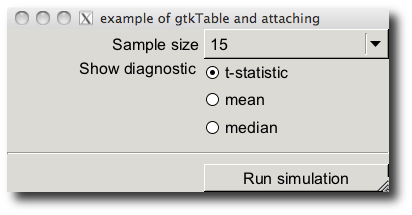
\includegraphics[width=.5\textwidth]{ex-RGtk2-dialog-layout}
  \caption{A basic dialog using a \code{gtkTable} container for layout.}
  \label{fig:RGtk2-dialog-layout}
\end{figure}

Our form layout will require $3$ rows and $2$ columns:
\begin{Schunk}
\begin{Sinput}
 tbl <- gtkTable(rows=3, columns=2, homogeneous=FALSE)
\end{Sinput}
\end{Schunk}
%
By default, the cells are allowed to have different sizes. This may be
overridden by passing \qcode{homogeneous = TRUE} to the constructor,
which forces all cells to have the same size.

We construct the widgets that will be placed in the form:
\begin{Schunk}
\begin{Sinput}
 sizeLabel <- gtkLabel("Sample size:")
 sizeCombo <- gtkComboBoxNewText()
 sapply(c(5, 10, 15, 30), sizeCombo$appendText)
 diagLabel <- gtkLabel("Diagnostic:")
 diagRadios <- gtkVBox()
 rb <- list()
 rb$t <- gtkRadioButton(label="t-statistic")
 rb$mean <- gtkRadioButton(rb, label="mean")
 rb$median <- gtkRadioButton(rb, label="median")
 sapply(rb, diagRadios$packStart)
 submitBox <- gtkVBox()
 submitBox$packEnd(gtkButton("Run simulation"), expand = FALSE)
\end{Sinput}
\end{Schunk}

The labels need to be aligned to the right, up against their
corresponding entry widgets, which should be left-aligned:
\begin{Schunk}
\begin{Sinput}
 sizeLabel['xalign'] <- 1
 diagLabel['xalign'] <- 1; diagLabel['yalign'] <- 0
 diagAlign <- gtkAlignment(xalign = 0)
 diagAlign$add(diagRadios)
\end{Sinput}
\end{Schunk}
% 
The labels are aligned through the \class{GtkMisc} functionality
inherited by \class{GtkLabel}. The \class{GtkVBox} with the radio
buttons does not support this, so we need to embed it within a
\class{GtkAlignment}. We have aligned the diagnostic label to the top
of its cell; otherwise, it would have been in the middle. The radio
buttons are left aligned, up against the label.

Child widgets are added to a table through the
\method{attach}{gtkTable} method.  The child can span more than one
cell. The arguments \argument{left.attach}{gtkTableAttach} and
\argument{right.attach}{gtkTableAttach} specify the horizontal bounds
of the child in terms of its left column and right column,
respectively. Analogously, \argument{top.attach}{gtkTableAttach} and
\argument{bottom.attach}{gtkTableAttach} define the vertical bounds.
By default, the widgets will expand into and fill the available space,
much as if \argument{expand}{gtkBoxPackStart} and
\argument{fill}{gtkBoxPackStart} were passed as \code{TRUE} to
\method{packStart}{GtkBox} (see
Section~\ref{sec:RGtk2:layout:box}). There is no padding between
children by default. Both the resizing behavior and padding may be
overridden by specifying additional arguments to
\method{attach}{GtkTable}.

The following attaches the combo box, radio buttons and their labels
to the table:
\begin{Schunk}
\begin{Sinput}
 tbl$attach(sizeLabel, left.attach=0,1, top.attach=0,1, 
            xoptions = c("expand", "fill"), yoptions="")
 tbl$attach(sizeCombo, left.attach=1,2, top.attach=0,1, 
            xoptions="fill", yoptions="")
 #
 tbl$attach(diagLabel, left.attach=0,1, top.attach=1,2, 
            xoptions = c("expand", "fill"), 
            yoptions=c("expand", "fill"))
 #
 tbl$attach(diagAlign, left.attach=1,2, top.attach=1,2, 
            xoptions=c("expand", "fill"), yoptions = "")
 #
 tbl$attach(submitBox, left.attach=1,2, top.attach=2,3, 
            xoptions="", yoptions=c("expand", "fill"))
\end{Sinput}
\end{Schunk}
%
The labels are allowed to expand and fill in the $x$ direction,
because correct alignment, to the right, requires them to have the
same size. The combo box is instructed to fill its space, as it would
otherwise be undesirably small, due to its short menu items. 

One can add spacing to the right of cells in a particular row or
column. Here we add $5$ pixels of space to the right of the label
column:
\begin{Schunk}
\begin{Sinput}
 tbl$setColSpacing(0, 5)
\end{Sinput}
\end{Schunk}

We complete the example by placing the table into a window:
\begin{Schunk}
\begin{Sinput}
 w <- gtkWindow(show=FALSE)
 w['border-width'] <- 14
 w$setTitle("GtkTable Example")
 w$add(tbl)
\end{Sinput}
\end{Schunk}

\end{example}


\chapter{RGtk2: Basic Components}
\label{sec:basic-components}


\section{Buttons}
\label{sec:RGtk2:gtkButton}

The button is the very essence of a GUI. It communicates its purpose
to the user and executes a command in response to a simple click or
key press. In \GTK\/, a basic button is usually constructed using
\constructor{gtkButton}, as the following example demonstrates.

\begin{example}{Button constructors}{eg:RGtk2:button-constructors}
\begin{Schunk}
\begin{Sinput}
 w <- gtkWindow(show=FALSE)
 w$setTitle("Various buttons")
 w$setDefaultSize(400, 25)
 g <- gtkHBox(homogeneous=FALSE, spacing=5)
 w$add(g)
 b <- gtkButtonNew() 
 b$setLabel("long way")
 g$packStart(b)
 g$packStart(gtkButton(label="label only") )
 g$packStart(gtkButton(stock.id="gtk-ok") )
 g$packStart(gtkButtonNewWithMnemonic("_Mnemonic") )
 w$show()
\end{Sinput}
\end{Schunk}
\end{example}

\begin{figure}
  \centering
  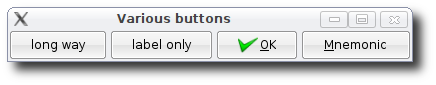
\includegraphics[width=.8\textwidth]{RGtk2-various-button}
  \caption{Various buttons}
  \label{fig:RGtk2:various-buttons}
\end{figure}

A \class{GtkButton} is simply a clickable region on the screen that is
rendered as a button. \class{GtkButton} is a subclass of
\class{GtkBin}, so it will accept any widget as an indicator of its
purpose. By far the most common button decoration is a label. The
first argument of \constructor{gtkButton},
\argument{label}{gtkButton}, accepts the text for an automatically
created \class{GtkLabel}. We have seen this usage in our ``Hello
World'' example and others.

Passing the \argument{stock.id}{gtkButton} argument to
\function{gtkButton} will use decorations associated with a so-called
stock identifier, see Section~\ref{sec:RGtk2:stock-icons}. For
example, ``gtk-ok'' would produce a button with a theme-dependent
image (such as a checkmark) and the ``Ok'' label, with the appropriate
mnemonic (see below) and language translation.  The available stock
identifiers are listed by \function{gtkStockListIds}.

The \constructor{gtkButtonNewWithMnemonic} constructor creates a
button with a mnemonic. A mnemonic is a key press that will activate
the button and is indicated by prefixing the character with an
underscore. In our example, we pass the string ``\_Mnemonic'', so
pressing \kbd{Alt-M} will effectively press the button.

%% signals
\paragraph{Signals}

The \signal{clicked} signal is emitted when the button is clicked with
the mouse, when the associated mnemonic is pressed or when the button
has focus and the \kbd{enter} key is pressed. A callback can listen
for this event to perform a command when the button is clicked.

\begin{example}{Callback example for
    \code{gtkButton}}{eg:RGtk2:gtkButton-callback}

\begin{Schunk}
\begin{Sinput}
 w <- gtkWindow(); b <- gtkButton("click me");
 w$add(b)
 ID <- gSignalConnect(b,"button-press-event",   # just mouse
                      f = function(w,e,data) {
                        print(e$getButton())    # which button
                        return(FALSE)           # propagate
                      })
 ID <- gSignalConnect(b,"clicked",              # keyboard too
                      f = function(w,...) {
                        print("clicked")
                      })
\end{Sinput}
\end{Schunk}
\end{example}

As buttons are intended to call an action immediately after being
clicked, it is advisable to make them insensitive to user input when
the action is not possible. For example, we could set our button to be
insensitive: 
\begin{Schunk}
\begin{Sinput}
 b$setSensitive(FALSE)
\end{Sinput}
\end{Schunk}

%% Buttons initiate actions
Windows often have a default action. For example, if a window contains
a form, the default action submits the form. If a button
executes the default action for the window, the button can be
set so that it is activated when the user presses \kbd{enter} while
the parent window has the focus. To implement this, the property
\code{can-default} must be \code{TRUE} and the widget method
\method{grabDefault}{gtkWidget} must be called. (This is not specific
to buttons, but any widget that can be activatable.) The
\class{GtkDialog} widget and its derivatives facilitate the use of
buttons in this manner, see Section~\ref{sec:dialogs}.

If the action that a button initiates is to be represented elsewhere
in the GUI, say a menu bar, then a \code{GtkAction} object may be
appropriate. Action objects are covered in
Section~\ref{sec:RGtk2:UIManager}.

\begin{example}{Spacing between buttons}{eg:RGtk2:mac-buttons}
This example shows how to pack buttons into a box so that the spacing
between the similar buttons is 12 pixels, while potentially dangerous
buttons are separated from the rest by 24 pixels, as per the Mac human
interface guidelines.  

\GTK\/ provides the widget \class{GtkHButtonBox} for organizing
buttons in a manner consistent across an application. However, the
default layout modes would not yield the desired spacing. As such, we
will illustrate how to customize the spacing.  We assume that our
parent container, \code{hbox}, is a horizontal box container.


\begin{figure}
  \centering
  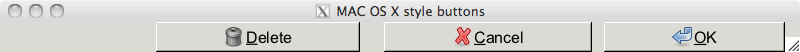
\includegraphics[width=.85\textwidth]{ex-RGtk2-mac-buttons}
  \caption{Example using stock buttons with extra spacing added between the \code{delete} and \code{cancel} buttons.}
  \label{fig:ex-RGtk2-mac-buttons}
\end{figure}

We include standard buttons, so we use the stock names and icons.
\begin{Schunk}
\begin{Sinput}
 cancel <- gtkButton(stock.id="gtk-cancel")
 ok <- gtkButton(stock.id="gtk-ok")
 delete <- gtkButton(stock.id="gtk-delete")
\end{Sinput}
\end{Schunk}

We specify the padding as we pack the widgets into the box, from right
to left, with \method{packEnd}{GtkBox}:
\begin{Schunk}
\begin{Sinput}
 hbox$packEnd(ok, padding=0)
 hbox$packEnd(cancel, padding=12)
 hbox$packEnd(delete, padding=12)
 hbox$packEnd(gtkLabel(""), expand=TRUE, fill=TRUE)
\end{Sinput}
\end{Schunk}
%
The padding occurs to the left and right of the child.  The \code{ok}
button is given no padding. The \code{cancel} button is packed with 12
pixels of spacing, which separates it from the \code{ok}
button. Recognizing the \code{delete} button as potentially
irreversible, we add 12 pixels of separation between it and the
\code{cancel} button, for a total of 24 pixels. The blank label pushes
the buttons against the right side of the box.  We instruct the
\code{ok} button to grab focus, so that it becomes the default
button:
\begin{Schunk}
\begin{Sinput}
 ok$grabFocus()
\end{Sinput}
\end{Schunk}






\end{example}

\section{Static Text and Images}

\subsection{Labels}
\label{sec:RGtk2:gtkLabel}

The primary purpose of a label is to communicate the role of another
widget, as we showed for the button. Labels are created by the
\constructor{gtkLabel} constructor, which takes the label text as its
first argument. This text can be set with either
\method{setLabel}{gtkLabel} or \method{setText}{gtkLabel} and
retrieved with either \method{getLabel}{gtkLabel} or
\method{getText}{gtkLabel}.  The difference being the former
respects formatting marks.

\begin{example}{Label formatting}{eg:RGtk2:label-formatting}
  As most text in a \GTK\/ GUI is ultimately displayed by
  \class{GtkLabel}, there are many formatting options available.  This
  example demonstrates a sample of
  these~(Figure~\ref{fig:RGtk2:label-formatting})
  
  \begin{figure}
    \centering
    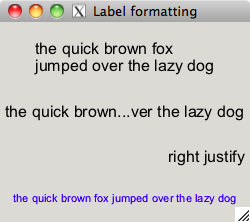
\includegraphics[width=.5\textwidth]{fig-RGtk2-labels}
    \caption{Various formatting for a label: wrapping, alignment,
      ellipsizing, PANGO markup}
    \label{fig:RGtk2:label-formatting}
  \end{figure}
  
\begin{Schunk}
\begin{Sinput}
 string <- "the quick brown fox jumped over the lazy dog"
 ## wrap by setting number of characters
 basicLabel <- gtkLabel(string)
 basicLabel$setLineWrap(TRUE)
 basicLabel$setWidthChars(35)            # no. characters
 ## Set ellipsis to shorten long text
 ellipsized <- gtkLabel(string)
 ellipsized$setEllipsize("middle")
 ## Right justify text lines
 ## use xalign property for aligning entire block
 rightJustified <- gtkLabel("right justify"); 
 rightJustified$setJustify("right")
 rightJustified['xalign'] <- 1
 ## PANGO markup
 pangoLabel <- gtkLabel()
 tmpl <- "<span foreground='blue' size='x-small'>%s</span>"
 pangoLabel$setMarkup(sprintf(tmpl, string))
 #
 sapply(list(basicLabel, ellipsized, rightJustified, pangoLabel), 
        g$packStart, expand = TRUE, fill = TRUE)
 w$showAll()
\end{Sinput}
\end{Schunk}
\end{example}

Many of the text formatting options are demonstrated in
Example~\ref{eg:RGtk2:label-formatting}. Line wrapping is enabled with
\method{setLineWrap}{gtkLabel}. Labels also support explicit line
breaks, specified with ``\code{\backslashn}.'' The
\method{setWidthChars}{gtkLabel} method is a convenience for instructing the
label to request enough space to show a specified number of
characters in a line.  When space is at a premium, long labels can be
ellipsized, i.e., have some of their text replaced with an
ellipsis, ``...''.  By default this is turned off; to enable, call
\method{setEllipsize}{gtkLabel}.  The property \code{justify}, with
values taken from \code{GtkJustification}, controls the alignment of
multiple lines within a label. To align the entire block of text
within the space allocated to the label, modify the \code{xalign}
property, as described in Section~\ref{sec:RGtk2:layout:align}.

\GTK\/ allows markup of text elements using the Pango text attribute
markup language, an XML-based format that resembles basic HTML. The
method \method{setMarkup}{gtkLabel} accepts text in the format. Text
is marked using tags to indicate the style. Some convenient tags are
\code{<b>} for bold, \code{<i>} for italics, \code{<ul>} for
underline, and \code{<tt>} for monospace text. Hyperlinks are possible
with \code{<a>}, as of version 2.18, and similar logic to
\function{browseURL} is implemented for launching a web
browser. Connect to the \signal{activate\_link} signal to
override it. More complicated markup involves the \code{<span>} tag
markup, such as \code{<span color='red'>some text</span>}. As with
HTML, the text may need to be escaped first so that designated
entities replace reserved characters.

Although mostly meant for static text display, \class{GtkLabel} has
some interactive features. If the \code{selectable} property is set to
\code{TRUE}, the text can be selected and copied into the clipboard.
Labels can hold mnemonics for other widgets; this is useful for
navigating forms. The mnemonic is specified at construction time with
\code{gtkLabelNewWithMnemonic}. The
\method{setMnemonicWidget}{gtkLabel} method identifies the widget to
which the mnemonic refers.

For efficiency reasons \class{GtkLabel} does not receive any input
events. It lacks an underlying \class{GdkWindow}, meaning that there
are no window system resources allocated for receiving the
events. Thus, to make a label interactive, one must first embed it
within a \class{GtkEventBox}, which provides the \class{GdkWindow}.

\subsection{Images}
\label{sec:RGtk2:images}

It is often said that a picture can be worth a thousand
words. Applying this to a GUI, images are often a more space efficient
alternative to labels. \class{GtkImage} is the widget that displays
images. The constructor \constructor{gtkImage} creates images from
various in-memory image representations, files, and other sources.
Images can be loaded after construction, as well. For example, the
\method{setFromFile}{gtkImage} method loads an image from a file.

\begin{example}{Using a pixmap to present graphs}{ex:RGtk2:pixbuf}





  This example shows how to use a \class{GtkImage} object to
  embed a graphic within \pkg{RGtk2}, using the
  \pkg{cairoDevice} package. The basic idea is to draw onto an
  off-screen pixmap using \pkg{cairoDevice} and
  then to construct a \class{GtkImage} from the pixmap. 

  We begin by creating a window of a certain size.
\begin{Schunk}
\begin{Sinput}
 w <- gtkWindow(show=FALSE); w$setTitle("Graphic window");
 w$setSizeRequest(400,400)
 hbox <- gtkHBox(); w$add(hbox)
 w$showAll()
\end{Sinput}
\end{Schunk}


The size of the image is taken as the size allocated to the box
\code{hbox}. This allows the window to be resized prior to drawing the
graphic. Unlike an interactive device, after drawing, this graphic
does not resize itself when the window resizes.
\begin{Schunk}
\begin{Sinput}
 theSize <- g$getAllocation()$allocation
 width <- theSize$width; height <- theSize$height
\end{Sinput}
\end{Schunk}

We create a \class{GdkPixmap} of the correct dimensions and
initialize an R graphics device that targets the pixmap. A simple
histogram is then plotted using base R graphics.
\begin{Schunk}
\begin{Sinput}
 require(cairoDevice)
 pixmap <- gdkPixmap(drawable = NULL, 
                     width = width, height = height, depth = 24)
 asCairoDevice(pixmap)
\end{Sinput}
\begin{Soutput}
[1] TRUE
\end{Soutput}
\begin{Sinput}
 hist(rnorm(100))
\end{Sinput}
\end{Schunk}

The final step is to create the \class{GtkImage} widget to display the
pixmap: 
\begin{Schunk}
\begin{Sinput}
 image <- gtkImage(pixmap = pixmap)
 hbox$packStart(image, expand=TRUE, fill = TRUE)
\end{Sinput}
\end{Schunk}

\end{example}


The image widget, like the label widget, does not have a parent
\class{GdkWindow}, which means it does not receive window events. As
with the label widget, the image widget can be placed inside a
\class{GtkEventBox} container if one wishes to connect to such
events.

\subsection{Stock icons}
\label{sec:RGtk2:stock-icons}

In \GTK\/, standard icons, like the one on the ``OK'' button, can be
customized by themes. This is implemented by a database that maps a
\textit{stock} identifier to an icon image. The stock identifier
corresponds to a commonly performed type of action, such as the ``OK''
response or the ``Save'' operation. There is no hard-coded set of
stock identifiers, however \GTK\/ provides a default set for the most
common operations. These identifiers are all prefixed with
``gtk-''. Users may register new types of stock icons.
%% ML: I believe there is an example of this in the RGtk2 demos

As mentioned previously, the full list of stock icons are returned in
a list by \function{gtkStockListIds}. The first $3$ are:
\begin{Schunk}
\begin{Sinput}
 head(unlist(gtkStockListIds()), n=3)   
\end{Sinput}
\begin{Soutput}
[1] "gtk-zoom-out" "gtk-zoom-in"  "gtk-zoom-fit"
\end{Soutput}
\end{Schunk}

The use of stock identifiers over specific images is encouraged, as it
allows an application to be customized through themes. The
\constructor{gtkButton} and \constructor{gtkImage} constructors accept
a stock identifier passed as \code{stock.id} argument, and the icons in
toolbars and menus are most conveniently specified by stock
identifier. 

% ML: Sorry, but I am not sure if this illustrates an important concept


% In the example below, we use the method \method{renderIcon}{gtkWidget} to
% return a pixbuf containing the icon that can be used with the
% constructor \constructor{gtkImageNewFromPixbuf} to display the
% icon. Here the stock id and size are specified to the
% \method{renderIcon}{gtkWidget} method.

% \begin{example}{\constructor{gtkButtonNewFromStock} -- the hard way}{ex:RGtk2:stock-icon}
% \SweaveInput{ex-RGtk2-button-new-stock-hardway}
% \end{example}

% ML: Could this example be in the book, but marked as optional or advanced?
%% JV Only for the package?? This will be placed in the package as an example.
% \begin{example}{Adding to the stock icons}{ex:RGtk2:add-stock-icons}
%   \SweaveInput{ex-RGtk2-add-stock-icon}
% \end{example}



%% Alertpanel application 
%% JV replaced this with one using reference Classes 
%% JV: This shows event boxes and reference classes, not a bad
%% thing but otherwise is just an info bar which isnow added. Should
%% we comment out?
%% ML: this is a fairly complicated example for a concept that is not
%% so important (GtkEventBox). I don't see how it's useful for
%% show/hide, which are pretty obvious.
%% JV: killed
% \begin{example}{An alert panel}{eg:RGtk2:alert-panel}
%   \SweaveInput{ex-RGtk2-alert-panel-2}
% \end{example}

\section{Input Controls}

\subsection{Text entry}
\label{sec:RGtk2:gtkEntry}

The widgets explained thus far are largely static. For example, \GTK\/
does not yet support editable labels. \GTK\/ has two different widgets
for editing text. One is optimized for multi-line text documents, the
other for single line entry. We will discuss complex multi-line text
editing in Section~\ref{sec:RGtk2:textviews}. For entering a single
line of text, the \class{GtkEntry} widget is appropriate:
\begin{Schunk}
\begin{Sinput}
 e <- gtkEntry()
\end{Sinput}
\end{Schunk}

The \code{text} property stores the text. This can be set with the
method \method{setText}{gtkEntry} and retrieved with
\method{getText}{gtkEntry}.  When the user has committed an entry,
e.g. by pressing the \kbd{enter} key, the \signal{activate} signal is
emitted. We connect to the signal and obtain the entered text upon
activation:
\begin{Schunk}
\begin{Sinput}
 gSignalConnect(e, "activate", function() {
   message("Text entered: ", e$getText())
 })
\end{Sinput}
\end{Schunk}

Sometimes the length of the text needs to be constrained to some
number of characters. The \argument{max}{gtkEntry} argument to
\function{gtkEntry} specifies this, but that usage is
deprecated. Instead, one should call \method{setMaxLength}{GtkEntry}.

\paragraph{The \class{GtkEditable} Interface}

Editing text programmatically relies on the \class{GtkEditable}
interface, which \class{GtkEntry} implements. The method
\method{insertText}{GtkEditable} inserts text before a position
specified by a $0$-based index. The return value is a list with the
component \code{position} indicating the position \textit{after} the
new text. The \method{deleteText}{GtkEditable} method deletes text
between two positions.

The example shows how to insert and then delete text:
\begin{Schunk}
\begin{Sinput}
 e$setText("Where did that guy go?")
 add.pos <- regexpr("guy", e['text']) - 1 # before "guy"
 ret <- e$insertText("@$#%! ", position = add.pos)
 e$getText()                             # or e['text']
\end{Sinput}
\begin{Soutput}
[1] "Where did that @$#%! guy go?"
\end{Soutput}
\begin{Sinput}
 e$deleteText(start = add.pos, end = ret$position)
 e$getText()
\end{Sinput}
\begin{Soutput}
[1] "Where did that guy go?"
\end{Soutput}
\end{Schunk}
% 

The \class{GtkEditable} interface supports three signals:
\signal{changed} when text is changed, \signal{delete-text} for delete
events, and \signal{insert-text} for insert events. It is possible to
prevent the insertion or deletion of text by connecting to the
corresponding signal and stopping the signal propagation with
\function{gSignalStopEmission}. 

\paragraph{Advanced \class{GtkEntry} Features}

\class{GtkEntry} has a number of features beyond basic text entry,
including: completion, buffer sharing, icons, and progress
reporting. We discuss completion in
Section~\ref{sec:RGtk2:entry-completion} and shared buffers in
Section~\ref{sec:RGtk2:buffer-sharing}. The progress reporting API,
introduced with version $2.16$, is virtually identical to that of
\class{GtkProgressBar}, introduced in
Section~\ref{sec:progress-bars}. We treat icons here. This feature has
been present since version $2.16$.

One can set an icon on an entry from a \class{GdkPixbuf}, stock ID,
icon name, or \class{GIcon}. Two icons are possible, one at the
beginning (\code{primary}) and one at the end (\code{secondary}). For
example, an entry might listen to its input and update its icon to
indicate whether the entered text is valid (in this case, consisting
only of letters):
%% JV: Cool, I didn't know this. The tooltip doesn't seem to work for
%% my setup.
\begin{Schunk}
\begin{Sinput}
 validatedEntry <- gtkEntry()
 gSignalConnect(validatedEntry, "changed", function(entry) {
   text <- entry$getText()
   if (nzchar(gsub("[a-zA-Z]", "", text))) {
     entry$setIconFromStock("primary", "gtk-no")
     validatedEntry$setIconTooltipText("primary", 
                                  "Only letters are allowed")
   }
   else { 
     entry$setIconFromStock("primary", "gtk-yes")
     validatedEntry$setIconTooltipText("primary", NULL)
   }
 })
 validatedEntry$setIconFromStock("primary", "gtk-yes")
\end{Sinput}
\end{Schunk}
%
We add a tooltip on the error icon to indicate the nature of the
problem to the user. Icons can also be made clickable and used as a
source for drag and drop operations.

\subsection{Check button}
\label{sec:RGtk2:gtkCheckbox}

Very often, the action performed by a button simply changes the value
of a state variable in the application. \GTK\/ defines several types
of buttons that explicitly manage and display one aspect of the
application state. The simplest type of state variable is binary
(boolean/logical) and is usually proxied by a \class{GtkCheckButton}.

A \class{GtkCheckButton} is constructed by
\function{gtkCheckButton}:
\begin{Schunk}
\begin{Sinput}
 cb <- gtkCheckButton("Option")
\end{Sinput}
\end{Schunk}
%
The state of the binary variable is represented by the
\code{active} property. We check our button:
\begin{Schunk}
\begin{Sinput}
 cb['active']
\end{Sinput}
\begin{Soutput}
[1] FALSE
\end{Soutput}
\begin{Sinput}
 cb['active'] <- TRUE
\end{Sinput}
\end{Schunk}

When the state is changed the \signal{toggle} signal is emitted. The
callback should check the \code{active} property to determine if the
button has been enabled or disabled:
\begin{Schunk}
\begin{Sinput}
 gSignalConnect(cb, "toggled", function(x) {
   message("Button is ", if (x$active) "active" else "inactive")
 })
\end{Sinput}
\end{Schunk}

An alternative to \class{GtkCheckButton} is the lesser used
\class{GtkToggleButton}, which is actually the parent class of
\class{GtkCheckButton}. A toggle button is drawn as an ordinary
button. It remains depressed while the state variable is \code{TRUE},
instead of relying on a check box to communicate the binary value.

\subsection{Radio button groups}
\label{sec:RGtk2:gtkRadioButton}

\GTK\/ provides two widgets for discrete state variables that accept
more than two possible values: combo boxes, discussed in the next
section, and radio buttons. The \function{gtkRadioButton} constructor
creates an instance of \class{GtkRadioButton}, an extension of
\class{GtkCheckButton}. Each radio button belongs to a group and only
one button in a group may be active at once.

\begin{example}{Basic Radio Button Usage}{eg:gtk:radio-group-group-list} 
  When we construct a radio button, we need to add it to a
  group. There is no explicit group object; rather, the buttons are
  chained together as a linked list. By default, a newly constructed
  button is added to its own group. If the group list is passed to the
  constructor, the newly created button is added to the group:
\begin{Schunk}
\begin{Sinput}
 labels <- c("two.sided", "less", "greater")
 radiogp <- list()                           # list for group
 radiogp[[labels[1]]] <- gtkRadioButton(label=labels[1]) 
 for(label in labels[-1]) 
   radiogp[[label]] <- gtkRadioButton(radiogp, label=label)
\end{Sinput}
\end{Schunk}
%
As a convenience, there are constructor functions ending with
\code{FromWidget} that determine the group from a radio button
belonging to the group. As we will see in our second example, this
allows for a more natural \function{sapply} idiom that avoids the need
to allocate a list and populate it in a \code{for} loop.

We add each button to a vertical box:
\begin{Schunk}
\begin{Sinput}
 w <- gtkWindow(); w$setTitle("Radio group example")
 g <- gtkVBox(FALSE, 5); w$add(g)
 sapply(radiogp, gtkBoxPackStart, object = g)
\end{Sinput}
\end{Schunk}

We can set and query which button is active:
\begin{Schunk}
\begin{Sinput}
 g[[3]]$setActive(TRUE)           
 sapply(radiogp, `[`, "active") 
\end{Sinput}
\begin{Soutput}
two.sided      less   greater 
    FALSE     FALSE      TRUE 
\end{Soutput}
\end{Schunk}

The \code{toggle} signal is emitted when a button is toggled. We need
to connect a handler to each button:
\begin{Schunk}
\begin{Sinput}
 sapply(radiogp, gSignalConnect, "toggled",     # connect each
        f = function(w, data) {
          if(w['active']) # set before callback
            message("clicked", w$getLabel(),"\n")
        })
\end{Sinput}
\end{Schunk}
\end{example}

\begin{example}{Radio Group via a \function{FromWidget}
    Constructor}{eg:gtk:radio-group-get-group}
  In this example, we illustrate using the
  \constructor{gtkRadioButtonNewWithLabelFromWidget} function to add
  new buttons to the group:
\begin{Schunk}
\begin{Sinput}
 radiogp <- gtkRadioButton(label=labels[1])
 btns <- sapply(labels[-1], gtkRadioButtonNewWithLabelFromWidget, 
                group = radiogp)
 w <- gtkWindow()
 w['title'] <- "Radio group example"
 g <- gtkVBox(); w$add(g)
 sapply(rev(radiogp$getGroup()), gtkBoxPackStart, object = g)
\end{Sinput}
\end{Schunk}
%
The \method{getGroup}{gtkRadioButton} method returns a list containing
the radio buttons in the same group. However, it is in the reverse
order of construction (newest first). This results from an internal
optimization that prepends, rather than appends, the buttons to a
linked list. Thus, we need to call \function{rev} to reverse the list
before packing the widgets into the box.

\end{example}

\subsection{Combo boxes}
\label{sec:RGtk2:basic:combobox}

The combo box is a more space efficient alternative to radio buttons
and is better suited for when there are a large number of options. A
basic, text-only \class{GtkComboBox} is constructed by
\constructor{gtkComboBoxNewText}. In
Section~\ref{sec:RGtk2:mvc:combobox} we will discuss combo boxes that
are based on an external data model.

We construct and populate a simple combo box:
\begin{Schunk}
\begin{Sinput}
 combo <- gtkComboBoxNewText()
 sapply(c("two.sided", "less", "greater"), combo$appendText)
\end{Sinput}
\end{Schunk}
%

The index of the currently active item is stored in the
\property{active}{gtkComboBox} property. The index, as usual, is $0$-based,
and a value of $-1$ indicates that no value is selected:
\begin{Schunk}
\begin{Sinput}
 combo['active']
\end{Sinput}
\begin{Soutput}
[1] -1
\end{Soutput}
\end{Schunk}
%
The \method{getActiveText}{gtkComboBox} method retrieves
the text shown by the basic combo box.

When the active index changes, the \signal{changed} signal is
emitted. The handler then needs to retrieve the active index:
\begin{Schunk}
\begin{Sinput}
 gSignalConnect(combo, "changed",
                f = function(w, ...) {
                  if(w$getActive() < 0) 
                    cat("No value selected\n")
                  else
                    cat("Value is", w$getActiveText(), "\n")
                })
\end{Sinput}
\end{Schunk}

Although combo boxes are much more space efficient than radio buttons,
it can be difficult to use a combo box when there are a large number
of items. The \method{setWrapWidth}{gtkComboBox} method specifies
the preferred number of columns for displaying the items.

\begin{example}{Using one combo box to populate another}{ex:RGtk2-comboboxes}
%
The goal of this example is to populate a combo box of variables
whenever a data frame is selected in another. We use two convenience
functions from the \pkg{ProgGUIInR} package to find the possible data
frames, and for a data frame to find its variables.

We create the two combo boxes and the enclosing window:
\begin{Schunk}
\begin{Sinput}
 w <- gtkWindow(show=FALSE)
 w$setTitle("gtkComboBox example")
 df_combo <- gtkComboBoxNewText()
 var_combo <- gtkComboBoxNewText()
\end{Sinput}
\end{Schunk}
%

Our layout uses boxes. To add a twist, we will hide our variable combo box
until after a data frame has been initially selected.
\begin{Schunk}
\begin{Sinput}
 g <- gtkVBox(); w$add(g)
 #
 g1 <- gtkHBox(); g$packStart(g1)
 g1$packStart(gtkLabel("Data frames:"))
 g1$packStart(df_combo)
 #
 g2 <- gtkHBox(); g$packStart(g2)
 g2$packStart(gtkLabel("Variable:"))
 g2$packStart(var_combo)
 g2$hide()
\end{Sinput}
\end{Schunk}
%

Finally, we configure the combo boxes. When a data frame is selected, we
first clear out the variable combo box and then populate it:
\begin{Schunk}
\begin{Sinput}
 sapply(avail_dfs(), df_combo$appendText)
 df_combo$setActive(-1)
 #
 gSignalConnect(df_combo, "changed", function(w, ...) {
   var_combo$getModel()$clear()
   sapply(find_vars(w$getActiveText()),  var_combo$appendText)
   g2$show()
 })
\end{Sinput}
\end{Schunk}
%


\end{example}

An extension of \class{GtkComboBox}, \class{GtkComboBoxEntry},
replaces the main button with a text entry. This supports the entry of
arbitrary values, in addition to those present in the menu.

\subsection{Sliders}
\label{sec:RGtk2:sliders}

The slider widget and spin button widget allow selection from a
regularly spaced, semi-continuous list of values.
\class{GtkScale} implements a slider and may be oriented
either horizontally or vertically. This depends on the class:
\class{GtkHScale} or \class{GtkVScale}.  

\begin{example}{A slider controlling histogram bin selection}{ex:RGtk2:sliders}
  We demonstrate a slider for controlling the bin size of a
  histogram. First, we create and configure the horizontal slider:
\begin{Schunk}
\begin{Sinput}
 slider <- gtkHScale(min = 1, max = 100, step = 1)
 slider$setValue(10)
 slider['value-pos'] <- "bottom"
\end{Sinput}
\end{Schunk}
%
We specify the minimum, maximum and step values for the scale.  This
set of values is formally represented by the \class{GtkAdjustment}
structure, which could serve as a data model for synchronizing multiple
sliders or other scale-based widgets. Ordinarily, it is not necessary
to construct a \class{GtkAdjustment} explicitly. Instead, one passes
the values as parameters to the constructor. The initial value is set
to $10$, and the value will be rendered in a label beneath the slider,
according to the \property{value-pos}{GtkScale} property.

The \signal{value-changed} signal is emitted whenever the slider is
adjusted. Our handler updates the histogram:
\begin{Schunk}
\begin{Sinput}
 gSignalConnect(slider, "value-changed",
                f = function(w, ...) {
                  val <- w$getValue() 
                  drawHistogram(val)
                })
\end{Sinput}
\end{Schunk}

Finally, we load the data, define the \function{drawHistogram}
function, and finish the GUI:
\begin{Schunk}
\begin{Sinput}
 data <- rnorm(100)
 library(lattice)
 drawHistogram <- function(val) print(histogram(data, nint = val))
 drawHistogram(slider$getValue())        
 w <- gtkWindow(); w$setTitle("Histogram bin selection")
 w$add(slider)
\end{Sinput}
\end{Schunk}
\end{example}

%% properties
A few properties define the appearance of the slider widget.  The
\code{digits} property controls the number of digits after the decimal
point.  The property \code{draw-value} toggles the drawing of the
selected value near the slider. Finally, \code{value-pos},
demonstrated above, specifies where this value will be drawn using
values from \code{GtkPositionType}. The default is \code{top}.

\subsection{Spin buttons}
\label{sec:RGtk2:spinboxes}

The spin button widget is very similar to the slider widget,
conceptually and in terms of the \GTK\/ API. Spin buttons are
constructed with \constructor{gtkSpinButton}. As with sliders, this
constructor requires specifying adjustment values, either as a
\class{GtkAdjustment} or individually.  The methods
\method{getValue}{gtkSpinButton} and \method{setValue}{gtkSpinButton}
once again get and set the value. The \code{value-changed}
signal is emitted when the spin button value is changed.

\begin{example}{A range widget}{ex:RGtk2-range-widget}
This example shows how to make a range widget that combines both the
slider and spinbutton to choose a single number. Such a widget is
useful, as the slider is better at large changes and the spin button
better at finer changes. In \GTK\/ we use the same
\class{GtkAdjustment} model, so changes to one widget propagate
without effort to the other.


We name our scale parameters according to the corresponding arguments
to the \function{seq} function:
\begin{Schunk}
\begin{Sinput}
 from <- 0; to <- 100; by <- 1
\end{Sinput}
\end{Schunk}

The slider is drawn without a value, as the value is already displayed
by the spin button. The call to \constructor{gtkHScale} implicitly
creates an adjustment for the slider. The spin button is then created
with the same adjustment.
\begin{Schunk}
\begin{Sinput}
 slider <- gtkHScale(min=from, max=to, step=by)
 slider['draw-value'] <- FALSE
 adjustment <- slider$getAdjustment()
 spinbutton <- gtkSpinButton(adjustment = adjustment)
\end{Sinput}
\end{Schunk}
%
Our layout places the two widgets in a horizontal box container with
the slider, but not the spin button, set to expand into the available
space.
\begin{Schunk}
\begin{Sinput}
 g <- gtkHBox()
 g$packStart(slider, expand=TRUE, fill=TRUE, padding=5)
 g$packStart(spinbutton, expand=FALSE, padding=5)
\end{Sinput}
\end{Schunk}


\end{example}

A spin button has a few additional features. The property
\code{snap-to-ticks} can be set to \code{TRUE} to force the new value
to belong to the sequence of values in the adjustment. The \code{wrap}
property indicates whether the sequence will ``wrap'' around at the
bounds.

\section{Progress Reporting}

\subsection{Progress bars}
\label{sec:progress-bars}

It is common to use a progress bar to indicate the progress of a long
running computation. This implemented by \class{GtkProgressBar}. A
text label describes the current operation, and the progress bar
communicates the fraction completed:
\begin{Schunk}
\begin{Sinput}
 w <- gtkWindow(); w$setTitle("Progress bar example")
 pb <- gtkProgressBar()
 w$add(pb)
 #
 pb$setText("Please be patient...")
 for(i in 1:100) {
   pb$setFraction(i/100)
   Sys.sleep(0.05) ## replace with a step in the process
 }
 pb$setText("All done.")
\end{Sinput}
\end{Schunk}

Progress bars can also show indefinite activity by periodically
pulsing the bar: 
\begin{Schunk}
\begin{Sinput}
 pb$pulse()
\end{Sinput}
\end{Schunk}

\subsection{Spinners}

Related to a progress bar is the \class{GtkSpinner} widget, which is a
graphical heartbeat to assure the user that the application is still
alive during long-running operations. Spinners are commonly found in
web browsers. The basic usage is straightforward:
\begin{Schunk}
\begin{Sinput}
 spinner <- gtkSpinner()
 spinner$start()
 spinner$stop()
\end{Sinput}
\end{Schunk}


\section{Wizards}
\label{sec:gtk-wizards}

The \class{GtkAssistant} class provides a wizard widget for \GTK. The
basic setup is one adds pages to the assistant object and they are
navigated in a linear manner. In our example, we will see how to
override this. 


Wizard pages have a certain type which must be declared. These are
enumerated in \code{GtkAssistantPageType} and set by \method{setPageType}{gtkAssistant}. The last page must be of
type \qcode{confirm}, \qcode{summary}, or \qcode{progress}.
Each wizard page has a content area and buttons.  As well, each page
in the assistant object has an optional side image, header image
and/or page title that may be customized. The buttons allow the user
to navigate through the wizard. The content area of a wizard page is
simply an instance of class \class{GtkWidget} (e.g., some container) and are
added to the assistant through the \method{appendPage}{gtkAssistant},
\method{insertPage}{gtkAssistant}, or
\method{prependPage}{gtkAssistant} methods. Pages are referred to by
the \class{GtkWidget} object or their page index, $0$-based. The
\code{forward} button on a page must be made sensitive by calling
\method{setPageComplete}{gtkAssistant} with the widget and logical
value.

%% signal
\paragraph{signals}
The \code{cancel} button emits a \signal{cancel} signal that can be
connected to for destroying the wizard widget. The \signal{apply}
signal is emitted on a page change. The \signal{prepare} signal is
emitted just before a page is made visible. This is needed to create
dynamically generated pages.

\begin{example}{An \code{install.packages} wizard}{eg-RGtk2-install-packages}

This example wraps the \function{install.packages} function into a
wizard with different pages for the (optional) selection of a CRAN
mirror, the selection of the package to install, the configuration
options provided and feedback. In general, wizards are quite common
for software installation.

We begin by defining our assistant and connecting to its
\signal{cancel} signal.
\begin{Schunk}
\begin{Sinput}
 asst <- gtkAssistant(show=FALSE)
 asst$setSizeRequest(500, 500)
 gSignalConnect(asst, "cancel", function(asst) asst$destroy())
\end{Sinput}
\end{Schunk}

Our pages will be computed dynamically. here we populate the pages
using box containers and specify their respective types. 
\begin{Schunk}
\begin{Sinput}
 pages <- lapply(1:5, gtkVBox, spacing=5, homogeneous=FALSE)
 page_types <- c("intro", rep("confirm",3), "summary")
 sapply(pages, gtkAssistantAppendPage, object=asst)
 sapply(pages, gtkAssistantSetPageType, object=asst, 
        type=page_types)
\end{Sinput}
\end{Schunk}
%
We customize each page with a logo, using a side log here.
\begin{Schunk}
\begin{Sinput}
 image <- gdkPixbuf(filename = imagefile("rgtk-logo.gif"))[[1]]
 sapply(pages, gtkAssistantSetPageSideImage, object=asst, 
        pixbuf=image)
\end{Sinput}
\end{Schunk}

When a page is about to be called we check and see if it has any
children, if not we call a function to create the page. These
functions are stored in a list so that they can be called by page index.
\begin{Schunk}
\begin{Sinput}
 populatePage <- list()                
 gSignalConnect(asst, "prepare", function(a, w, data) {
   page_no <- which(sapply(pages, identical, w))
   if(!length(w$getChildren()))
     populatePage[[page_no]]()
 })
\end{Sinput}
\end{Schunk}

Although we don't show how to create the CRAN selection page
(cf. Example~\ref{ex:RGtk2-add-toggle-to-df} for a similar
construction) we call \method{setForwardPageFunc}{gtkAssistant} to set
a function that will skip this page if it is not needed. This function
simply returns an integer with the next page number based on the last one.
\begin{Schunk}
\begin{Sinput}
 asst$setForwardPageFunc(function(i, data) {
   ifelse(i == 0 && have_CRAN(), 2L, as.integer(i + 1))
 }, data=NULL)
\end{Sinput}
\begin{Soutput}
NULL
\end{Soutput}
\end{Schunk}

We have a few script globals that allow us to pass data between pages.
\begin{Schunk}
\begin{Sinput}
 CRAN_package <- NA
 install_options <- list() #type, dependencies, lib
\end{Sinput}
\end{Schunk}






We now show how some of the pages are populated. The initial screen is
a welcome and simply shows a label. It is immediately complete.

\begin{Schunk}
\begin{Sinput}
 populatePage[[1]] <- function() {
   asst$setPageTitle(pages[[1]], "Install a CRAN package")
   pages[[1]]$packStart(l <- gtkLabel())
   pages[[1]]$packStart(gtkLabel(), expand=TRUE) # a spring
   
   l$setMarkup(paste(
        "<span font='x-large'>Install a CRAN package</span>",
        "This wizard will help install a package from <b>CRAN</b>",
        "If you have not already specified a CRAN repository, one",
        "you will be prompted to do so.",
        sep="\n"))
   asst$setPageComplete(pages[[1]], TRUE)
 }
\end{Sinput}
\end{Schunk}


  
  

We skip showing the pages to select a CRAN site and a package, as they
are based on the forthcoming \class{GtkTreeView} class. On the
fourth page is a summary of the package taken from CRAN and a chance
for the user to configure a few options for \function{install.packages}.
\begin{Schunk}
\begin{Sinput}
 populatePage[[4]] <- function() {
   asst$setPageTitle(pages[[4]], "Install CRAN package")
   #
   get_desc <- function(pkgname) {
     tpl <- "http://cran.r-project.org/web/packages/%s/DESCRIPTION"
     x <- readLines(sprintf(tpl, pkgname))
     f <- tempfile(); cat(paste(x, collapse="\n"), file=f)
     read.dcf(f)
   }
   pkg_desc <- get_desc(CRAN_package)
   #
   l <- gtkLabel()
   l$setMarkup(paste(
     sprintf("Install package: <b>%s</b>", pkg_desc[1, 'Package']),
     "\n",
     sprintf("%s", pkg_desc[1, 'Description']),
     sep="\n"))
   
   pages[[4]]$packStart(l)
   #
   tbl <- gtkTable()
   pages[[4]]$packStart(tbl, expand=FALSE)
   pages[[4]]$packStart(gtkLabel(), expand=TRUE)
   
   #
   combo <- gtkComboBoxNewText()
   pkg_types <- c("source", "mac.binary", "mac.binary.leopard",
                  "win.binary", "win64.binary")
   sapply(pkg_types, combo$appendText)
   combo$setActive(which(getOption("pkgType") == pkg_types) - 1)
   gSignalConnect(combo, "changed", function(w, ...) {
     install_options[['type']] <<- pkg_types[1 + w$getActive()]
   })
   tbl$attachDefaults(gtkLabel("Package type:"), 0, 1, 0, 1)
   tbl$attachDefaults(combo, 1, 2, 0, 1)
 
   #
   cb <- gtkCheckButton()
   cb$setActive(TRUE)
   gSignalConnect(cb, "toggled", function(w) {
     install_options[['dependencies']] <<- w$getActive()
   })
   tbl$attachDefaults(gtkLabel("Install dependencies"), 0, 1, 1, 2)
   tbl$attachDefaults(cb, 1, 2, 1, 2)
 
   #
   fc <- gtkFileChooserButton("Select a directory...", 
                              "select-folder")
   fc$setFilename(.libPaths()[1])
   gSignalConnect(fc, "selection-changed", function(w) {
     dir <- w$getFilename()
     install_options[['lib']] <<- dir
   })
   tbl$attachDefaults(gtkLabel("Where"), 0, 1, 2, 3)
   tbl$attachDefaults(fc, 1, 2, 2, 3)
 
   asst$setPageComplete(pages[[4]], TRUE)
 }
\end{Sinput}
\end{Schunk}

Our last page, where the selected package is installed, would
naturally be of type \code{progress}, but there is no means to
interrupt the flow of \function{install.packages} to update the
page. A real application would reimplement that. Instead we just set a
message once the package install attempt is done.
\begin{Schunk}
\begin{Sinput}
 populatePage[[5]] <- function() {
   asst$setPageTitle(pages[[5]], "Done")
   install_options$pkgs <- CRAN_package
   out <- try(do.call("install.packages", install_options), 
              silent=TRUE)
 
   l <- gtkLabel(); pages[[5]]$packStart(l)
   if(!inherits(out, "try-error")) {
     l$setMarkup(sprintf("Package %s installed successfully", 
                         CRAN_package))
   } else {
     l$setMarkup(paste(sprintf("Package %s failed to install", 
                               CRAN_package),
                       paste(out, collapse="\n"),
                       sep="\n"))
   }
 
   asst$setPageComplete(pages[[5]], FALSE)
 }
\end{Sinput}
\end{Schunk}

To finish we simply need to populate the first page and call the
assistant's \meth{show} method.
\begin{Schunk}
\begin{Sinput}
 populatePage[[1]]()
 asst$show()
\end{Sinput}
\end{Schunk}
\end{example}

\section{Embedding R Graphics}
\label{sec:gtk-widget-graphics}

%% using cairoDevice to embed graphics
%% cairoDevice

The package \pkg{cairoDevice} is an R graphics device based on the
Cairo graphics library.  It supports alpha-blending and antialiasing
and reports user events through the \function{getGraphicsEvent}
function. \pkg{RGtk2} and \pkg{cairoDevice} are integrated through the
\function{asCairoDevice} function. If a \class{GtkDrawingArea},
\class{GdkDrawable}, \class{Cairo} context, or \class{GtkPrintContext}
is passed to \function{asCairoDevice}, an R graphics device will be
initialized that targets its drawing to the object. For simply
displaying graphics in a GUI, the \class{GtkDrawingArea} is the best
choice. 

This is the simplest usage:
\begin{Schunk}
\begin{Sinput}
 library(cairoDevice)
 device <- gtkDrawingArea()
 asCairoDevice(device)
\end{Sinput}
\begin{Soutput}
[1] TRUE
\end{Soutput}
\begin{Sinput}
 win <- gtkWindow(show=FALSE)
 win$add(device)
 win$showAll()
 plot(mpg ~ hp, data = mtcars)
\end{Sinput}
\end{Schunk}
%
We create the \class{GtkDrawingArea}, coerce it to a Cairo-based
graphics device, and place it in a window. Finally, we display a
scatterplot. Example~\ref{sec:RGtk2:scroll-windows} goes further by
embedding the drawing area into a scrolled window to support zooming
and panning.

For more complex use cases, such as compositing a layer above or below
the R graphic, one should pass an off-screen \class{GdkDrawable}, like
a \class{GdkPixmap}, or a \class{Cairo} context. The off-screen
drawing could then be composited with other images when
displayed. Example~\ref{ex:RGtk2:pixbuf} generates an icon by pointing
the device to a pixmap. Finally, passing a \class{GtkPrintContext} to
\function{asCairoDevice} allows printing R graphics through the \GTK\/
printing dialogs.

\begin{example}{Printing R Graphics}{eg:RGtk2:printing-graphics}
  This example will show how to use the printing support in \GTK\/ for
  printing an R plot. 
  
  A print operation is encapsulated by \class{GtkPrintOperation}:
\begin{Schunk}
\begin{Sinput}
 printOp <- gtkPrintOperation()
\end{Sinput}
\end{Schunk}
%
A print operation may perform several different actions: print
directly, print through a dialog, show a print preview and export to a
file. Before performing any such action, we need to implement the
rendering of our document into printed form. This is accomplished by
connecting to the \signal{draw-page} signal. The handler is passed a
\class{GtkPrintContext}, which contains the target Cairo context. In
general, one would call Cairo functions to render the document, which
is beyond our scope. In this case, though, we can pass the context
directly to \pkg{cairoDevice} for rendering the R plot:
\begin{Schunk}
\begin{Sinput}
 gSignalConnect(printOp, "draw-page", function(x, context, page_nr) {
   asCairoDevice(context)
   plot(mpg ~ wt, data = mtcars)
 })
\end{Sinput}
\end{Schunk}
%
  The final step is to run the operation to perform one of the
  available actions. In this example, we launch a print dialog:
\begin{Schunk}
\begin{Sinput}
 printOp$run(action = "print-dialog", parent = NULL)
\end{Sinput}
\end{Schunk}
% 
  When the user confirms the dialog, the
  \signal{draw-page} handler is invoked, and the
  rendered page is sent to the printer.
\end{example}

\section{Drag and drop}
\label{sec:RGtk2:dnd}

%% ------------ Drag and Drop

A drag and drop operation is the movement of data from a source widget
to a target widget. The source widget serializes the selected item as
MIME data, and the destination interprets that data to perform some
operation, often creating an item of its own. Our task is to configure
the source and destination widgets, so that they listen for the
appropriate events and understand each other. As a trivial example, we
allow the user to drag the text from one button to another.

\subsection{Initiating a Drag}

When a drag and drop is initiated, different types of data may be
transferred. We need to define a target type for each type of data, as
a \class{GtkTargetEntry} structure:
\begin{Schunk}
\begin{Sinput}
 TARGET.TYPE.TEXT   <- 80                 
 TARGET.TYPE.PIXMAP <- 81                  
 widgetTargetTypes <- 
   list(text = gtkTargetEntry("text/plain", 0, 
          TARGET.TYPE.TEXT),
        pixmap = gtkTargetEntry("image/x-pixmap", 0, 
          TARGET.TYPE.PIXMAP))
\end{Sinput}
\end{Schunk}
%
The first component of \class{GtkTargetEntry} is the name, which is often
a MIME type. The flags come next, which are usually left at $0$, and
finally we specify an arbitrary identifier for the target. We will
only use the \qcode{text} target in this example.

We construct a button and call \function{gtkDragSourceSet} to instruct
it to act as a drag source:
\begin{Schunk}
\begin{Sinput}
 w <- gtkWindow(); w['title'] <- "Drag Source"
 dragSourceWidget <-  gtkButton("Text to drag")
 w$add(dragSourceWidget)
 gtkDragSourceSet(dragSourceWidget,
        start.button.mask=c("button1-mask", "button3-mask"),
        targets=widgetTargetTypes[["text"]],
        actions="copy")
\end{Sinput}
\end{Schunk}
%
The \argument{start.button.mask}{gtkDragSourceSet}, with values from
\class{GdkModifierType}, indicates the modifier buttons that need to
be pressed to initiate the drag. The allowed target is \qcode{text} in
this case. The \argument{actions}{gtkDragSourceSet} argument lists the
supported actions, such as \code{copy} or \code{move}, from the
\class{GdkDragAction} enumeration.

When a drag is initiated, we will receive the \signal{drag-data-get}
signal, which needs to place some data into the passed
\class{GtkSelectionData} object:
\begin{Schunk}
\begin{Sinput}
 gSignalConnect(dragSourceWidget, "drag-data-get", 
                function(widget, context, sel, tType, eTime) {
                  sel$setText(widget$getLabel()) 
                })
\end{Sinput}
\end{Schunk}
%
If we had allowed the \code{move} action, we would also need to
connect to \signal{drag-data-delete}, in order to delete the data that
was moved away.

\subsection{Handling Drops}

In a separate window from the drag source button, we construct another
button and call \function{gtkDragDestSet} to mark it as a drag target:
\begin{Schunk}
\begin{Sinput}
 w <- gtkWindow(); w['title'] <- "Drop Target"
 dropTargetWidget <- gtkButton("Drop here")
 w$add(dropTargetWidget)
 gtkDragDestSet(dropTargetWidget,
                flags="all", 
                targets=widgetTargetTypes[["text"]],
                actions="copy")
\end{Sinput}
\end{Schunk}
%
The signature is similar to that of \function{gtkDragSourceSet},
except for the \argument{flags}{gtkDragDestSet} argument, which
indicates which operations, of the set \code{motion}, \code{highlight}
and \code{drop}, \GTK\/ will handle with reasonable default
behavior. Specifying \code{all} is the most convenient course, in
which case we only need to implement the extraction of the data from
the \class{GtkSelectionData} object. For a drop to occur, there must be a
non-empty intersection between the targets passed to
\function{gtkDragSourceSet} and those passed to
\function{gtkDragDestSet}.

When data is dropped, the destination widget emits the
\signal{drag-data-received} signal. The handler is responsible for
extracting the dragged data from \argument{selection} and performing some
operation with it. In this case, we set the text on the button:
\begin{Schunk}
\begin{Sinput}
 gSignalConnect(dropTargetWidget, "drag-data-received", 
        function(widget, context, x, y, sel, tType, eTime) {
          dropdata <- sel$getText()
          widget$setLabel(rawToChar(dropdata))
        })
\end{Sinput}
\end{Schunk}
%
The \argument{context} argument is a \class{GdkDragContext},
containing information about the drag event. The \argument{x} and
\argument{y} arguments are integer valued and represent the position
in the widget where the drop occurred. The text data is returned by
\function{getText} as a \code{raw} vector, so it is converted with
\function{rawToChar}.

%% JV: This could be expanded -- motion is not covered, as is done with
%% tcltk, but I don't think it is needed without a compelling use case.

%% ML: agreed

\chapter{RGtk2: Widgets Using Data Models}
\label{sec:RGtk2:widgets-with-models}

%% Possible outline:
%% - Displaying tabular data (GtkTreeView)
%%   - Loading data frame
%%   - Displaying data frame
%%   - Accessing GtkTreeModel (to set up selection, and hierarchical data)
%%   - Selection (an important concept, but common to hierarchical, below)
%%   - Sorting/filtering
%%   - Cell renderer details
%% - Displaying hierarchical data (GtkTreeView)
%%   - Loading hierarchical data
%%   - Displaying data as a tree
%% - Model-based combo boxes
%% - Text entry completion
%% - Icon views (currently omitted, probably OK)
%% - Text views

%% TODO: we need a unified example in the main text that spans loading
%% a data frame to sorting a model, at least.

Many widgets in \GTK\/ use the model, view, controller (MVC)
paradigm. For most, like the button, the MVC pattern is implicit;
however, widgets that primarily display data explicitly incorporate
the MVC pattern into their design. The data model is factored out as a
separate object, while the widget plays the role of the view and
controller. The MVC approach adds a layer of complexity but
facilitates the display of the dynamic data in multiple, coordinated
views.

\section{Display of tabular data}
\label{sec:RGtk2:tabular-heirarchical-data}

Widgets that display lists, tables and trees are all based on the same
basic data model, \class{GtkTreeModel}. Although its name suggests a
hierarchical structure, \class{GtkTreeModel} is also tabular. We first
describe the display of an \R\/ data frame in a list or table
view. The display of hierarchical data, as well as further details of
the \class{GtkTreeModel} framework, are treated subsequently.

\subsection{Loading a data frame}
\label{sec:tabular-stores-tree}

As an interface, \class{GtkTreeModel} may be implemented in any number
of ways. \GTK\/ provides simple in-memory implementations for
hierarchical and non-hierarchical data. For improved speed,
convenience and familiarity, \pkg{RGtk2} includes a custom
\class{GtkTreeModel} implementation called \class{RGtkDataFrame}, which
is based on an \R\/ data frame. For non-hierarchical data, this is
usually the model of choice, so we discuss it first.

\R\/ uses data frames to hold tabular data, where each column is of a
certain class, and each row is related to some observational
unit. This fits the structure of \class{GtkTreeModel} when there is no
hierarchy. As such it is natural to have a means to map a data frame
into a store for a tree view. \class{RGtkDataFrame} implements
\class{GtkTreeModel} to perform this role and is constructed with the
\constructor{rGtkDataFrame} function. Populating a
\class{RGtkDataFrame} is far faster than for a \GTK\/ model, because
data is retrieved from the data frame on demand. There is no need to
copy the data row by row into a separate data structure. Such an
approach would be especially slow if implemented as a loop in \R. The
constructor takes a data frame as an argument. The column classes are
important, so even if this data frame is empty, the user should
specify the desired column classes upon construction.

An object of class \class{RGtkDataFrame} supports the familiar S3
methods \method{[}{RGtkDataFrame}, \method{[\ASSIGN}{RGtkDataFrame},
\method{dim}{RGtkDataFrame}, and
\method{as.data.frame}{RGtkDataFrame}. The \code{[$<$-} method does
not have quite the same functionality as it does for a data
frame. Columns can not be removed by assigning values to \code{NULL},
and column types should not be changed. These limitations are inherit
in the design of \GTK: columns may not be removed from
\class{GtkTreeModel}, and views expect the data type to remain the
same.

\begin{example}{Defining and manipulating a \class{RGtkDataFrame}}{eg-RGtk2-manipulate-rGtkDataframe}
  The basic data frame methods are similar.
\begin{Schunk}
\begin{Sinput}
 data(Cars93, package="MASS")             # mix of classes
 model <- rGtkDataFrame(Cars93)
 model[1, 4] <- 12
 model[1, 4]                              # get value
\end{Sinput}
\begin{Soutput}
[1] 12
\end{Soutput}
\end{Schunk}
%
As with a data frame, assignment to a factor must be from one of the
possible levels.

\end{example}

The data frame combination functions \Rfunction{rbind} and
\Rfunction{cbind} are unsupported, as they would create a new data
model, rather than modify the model in place. Thus, one should add
rows with \method{appendRows}{rGtkDataFrame} and add columns with
\method{appendColumns}{rGtkDataFrame} (or sub-assignment, 
\method{[\ASSIGN}{RGtkDataFrame}).

The \method{setFrame}{rGtkDataFrame} method replaces the underlying
data frame.
\begin{Schunk}
\begin{Sinput}
 model$setFrame(Cars93[1:5, 1:5])
\end{Sinput}
\end{Schunk}
%
Replacing the data frame is the only way to remove rows, as this is
not possible with the conventional data frame sub-assignment
interface. Removing columns or changing their types remains
impossible. The new data frame cannot contain more columns and rows
than the current one. If the new data frame has more rows or columns,
then the appropriate \code{append} method should be used first.

\subsection{Displaying data as a list or table}
\label{sec:RGtk2:mvc:GtkTreeView}

%% intro
\class{GtkTreeView} is the primary view of \class{GtkTreeModel}.  It
serves as the list, table and tree widget in \GTK. A tree view is
essentially a container of columns, where every column has the same
number of rows. If the view has a single column, it is essentially a
list. If there are multiple columns, it is a table. If the rows are
nested, it is a tree table, where every node has values on the same
columns.

%% constructor
A tree view is constructed by \constructor{gtkTreeView}:
\begin{Schunk}
\begin{Sinput}
 view <- gtkTreeView(model)
\end{Sinput}
\end{Schunk}
Usually, as in the above, the model is passed to the
constructor. Otherwise, the model may be accessed with
\method{setModel}{gtkTreeView} and \method{getModel}{gtkTreeView}.

A newly created tree view displays zero columns, regardless of the
number of columns in the model. Each column, an instance of
\class{GtkTreeViewColumn}, must be constructed, inserted into the view and
instructed to render content based on one or more columns in the data
model:
\begin{Schunk}
\begin{Sinput}
 vc <- gtkTreeViewColumn()
 vc$setTitle("Manufacturer")
 cr <- gtkCellRendererText()
 vc$packStart(cr)
 vc$addAttribute(cr, "text", 0)
 view$insertColumn(vc, 0)
\end{Sinput}
\end{Schunk}
%
A column with the title ``Manufacturer'' is inserted at the first,
$0$-based, position. For displaying a simple data frame, we only need
to render text. Each row in a column consists of one or more cells,
managed in a layout. The number of cells and how each cell is rendered
is uniform down a column. As an implementation of
\class{GtkCellLayout}, \class{GtkTreeViewColumn} delegates the
responsibility of rendering to one or more \class{GtkCellRenderer}
objects. The cell renderers are packed into the column, which behaves
much like a box container. Rendering of text cells is the role of
\class{GtkCellRendererText}; we create an instance with
\constructor{gtkCellRendererText}. There are several properties that
control how the text is rendered. A so-called \textit{attribute} links
a model column to a renderer property. The most important property is
\code{text}, the text itself. In the example, we bind the \code{text}
property to the first ($0$-indexed) column in the model.

\class{GtkTreeView} provides the
\method{insertColumnWithAttributes}{gtkTreeView} convenience method to
perform all of these steps with a single call. We invoke it to add a
second column in our view:
\begin{Schunk}
\begin{Sinput}
 view$insertColumnWithAttributes(position = -1, 
      title = "Model", cell = gtkCellRendererText(), text = 1)
\end{Sinput}
\end{Schunk}
% 
The $-1$ passed as the first argument indicates that the column should
be appended. Next, we specify the column title, a cell renderer, and
an attribute that links the \code{text} renderer property to the
second column in the model. In general, any number of attributes may
be defined after the third argument.  We will use the above idiom in
all of the following examples, as it is much more concise than
performing each step separately.

To display the entire Cars93 data frame, we insert a view column for
every column in the data frame. Here, we reconstruct the view, inserting
a view column for every column in the data frame, i.e., the model.
\begin{Schunk}
\begin{Sinput}
 view <- gtkTreeView(model)
 mapply(view$insertColumnWithAttributes,  -1, colnames(model), 
        list(gtkCellRendererText()), 
        text = seq_len(ncol(model)) - 1)
\end{Sinput}
\end{Schunk}
%
Although it was relatively easy to create a \class{GtkTreeModel} for
the data frame using \class{RGtkDataFrame}, the complexity of
\class{GtkTreeView} complicates the task of displaying the data frame
in a simple, textual table. When this is all that is necessary, one
might consider \function{gtable} from \pkg{gWidgets}. For those
who wish to render text in each row differently (e.g., in a different
color) or fill cells with images, check boxes, progress bars and the
like, direct use of the \class{GtkTreeView} API is required.

\paragraph{Manipulating view columns}
The \class{GtkTreeView} widget is essentially a collection of
columns. Columns are added to the tree view with the methods
\method{insertColumn}{gtkTreeView} or, as shown above,
\method{insertColumnWithAttributes}{gtkTreeView}.  A column can be
moved with the \method{moveColumnAfter}{gtkTreeView} method, and
removed with the \method{removeColumn}{gtkTreeView} method. The
\method{getColumns}{gtkTreeView} method returns a list containing all
of the tree view columns.

There are several properties for controlling the behavior and
dimensions of a \class{GtkTreeViewColumn} instance. The property
\qcode{resizable} determines whether the user can resize a column, by
dragging with the mouse. The size properties \qcode{width},
\qcode{min-width}, and \qcode{fixed-width} control the size. The
visibility of the column can be adjusted through the
\method{setVisible}{gtkTreeViewColumn} method.

\paragraph{Additional Features}

Tree views have several special features, including sorting,
incremental search and drag-n-drop reordering. Sorting is discussed in
Section~\ref{sec:RGtk2:mvc:proxies}. To turn on searching,
\code{enable-search} should be \code{TRUE} (the default) and the
\code{search-column} property should be set to the column to be
searched. The tree view will popup a search box when the user types
\kbd{control-f}. To designate an arbitrary text entry widget as the
search box, call \method{setSearchEntry}{GtkTreeView}. The entry can
be placed anywhere in the GUI. Columns are always reorderable by drag
and drop. Reordering rows through drag-and-drop is enabled by the
\code{reorderable} property.

\paragraph{Aesthetic properties}

\class{GtkTreeView} is capable of rendering some visual guides. The
\code{rules-hint}, if \code{TRUE}, will instruct the theme to draw
rows in alternating colors. To show grid lines, set
\code{enable-grid-lines} to \code{TRUE}.

\subsection{Accessing \class{GtkTreeModel}}
\label{sec:RGtk2:mvc:iterators}

Although \class{RGtkDataFrame} provides a familiar interface for
manipulating the data in a \class{GtkTreeModel}, it is often necessary
to directly interact with the \GTK\/ API, such as when using another
type of data model or interpreting user selections. There are two
primary ways to index into the rows of a tree model: paths and
iterators.

To index directly into an arbitrary row, a \class{GtkTreePath} is
appropriate. For a table, a tree path is essentially the row number,
$0$-based; for a tree it is a sequence of integers referring to the
offspring index at each level. The sequence of integers may be
expressed as either a numeric vector or a string, using
\constructor{gtkTreePathNewFromIndices} or
\constructor{gtkTreePathNewFromString}, respectively. For a flat table
model, there is only one integer in the sequence:
\begin{Schunk}
\begin{Sinput}
 secondRow <- gtkTreePathNewFromIndices(2)
\end{Sinput}
\end{Schunk}
%
Referring to a row in a hierarchy is slightly more complex:
\begin{Schunk}
\begin{Sinput}
 abcPath <- gtkTreePathNewFromIndices(c(1, 3, 2))
 abcPath <- gtkTreePathNewFromString("1:3:2")
\end{Sinput}
\end{Schunk}
%
In the above, both paths refer to the second child of the third child
of the first top-level node. To recover the integer or string
representation of the path, use \method{getIndices}{GtkTreePath} or
\method{toString}{GtkTreePath}, respectively.

%% iters

The second means of row indexing is through an iterator,
\class{GtkTreeIter}, which is better suited for traversing a model.
While a tree path is an intuitive, transparent row index, an iterator
is an opaque index that is efficiently incremented. It is
probably most common for a model to be accessed in an iterative
manner, so all of the data accessor methods for \class{GtkTreeModel}
expect \class{GtkTreeIter}, not \class{GtkTreePath}. The \GTK\/
designers imagined that the typical user would obtain an iterator for
the first row and visit each row in sequence:
\begin{Schunk}
\begin{Sinput}
 iter <- model$getIterFirst()
 manufacturer <- character()
 while(iter$retval) {
   manufacturer <- c(manufacturer, model$get(iter$iter, 0)[[1]])
   iter$retval <- model$iterNext(iter$iter)
 }
\end{Sinput}
\end{Schunk}
%
In the above, we recover the manufacturer column from the Cars93 data
frame. Whenever a \class{GtkTreeIter} is returned by a
\class{GtkTreeModel}, the return value in \R\/ is a list of two
components: \code{retval}, a logical indicating whether the iterator
is valid, and \code{iter}, the pointer to the underlying C data
structure. The call to \method{get}{GtkTreeModel} also returns a list,
with an element for each column index passed as an argument. The
method \method{iterNext}{gtkTreeStore} updates the passed iterator in
place, i.e., by reference, to point to the next row. Thus, no new
iterator is returned. This is unfamiliar behavior in \R. Instead, the
method returns a logical value indicating whether the iterator is
still valid, i.e. \code{FALSE} is returned if no next row exists.

It is clear that the above usage is designed for languages like C,
where multiple return values are conveniently passed by reference
parameters. The iterator design also prevents the use of the apply
functions, which are generally preferred over the \code{while} loop
for reasons of performance and clarity. An improvement would be to
obtain the number of children, generate the sequence of row indices
and access the row for each index:
\begin{Schunk}
\begin{Sinput}
 nrows <- model$iterNChildren(NULL)
 manufacturer <- sapply(seq(nrows), function(i) {
   iter <- model$iterNthChild(NULL, i)
   model$get(iter$iter, 0)[[1]]
 })
\end{Sinput}
\end{Schunk}
%
Here we use \code{NULL} to refer to the virtual root node that sits
above the rows in our table. Unfortunately, this usage too is
unintuitive and slow, so the benefits of \class{RGtkDataFrame} should
be obvious.

One can convert between paths and iterators. The method
\method{getIter}{GtkTreeModel} on \class{GtkTreeModel} returns an
iterator for a path. A shortcut from the string representation of the
path to an iterator is \method{getIterFromString}{GtkTreeModel}. The
path pointed to by an iterator is returned by
\method{getPath}{GtkTreeModel}.

One final point: \class{GtkTreeIter} is created and managed by the
model, while \class{GtkTreePath} is model independent. It is not
possible to use iterators across models or even across modifications
to a model. After a model changes, an iterator is invalid. A tree path
may still point to a valid row, though it will not in general be the
same row from before the change. To refer to the same row across tree
model changes, use a \class{GtkTreeRowReference}.

\subsection{Selection}
%% selection: none, single browse multiple, getSelected

There are multiple modes of user interaction with a tree view: if the
cells are not editable, then selection is the primary mode.  A single
click selects the value, and a double click is often used to initiate
an action. If the cells are editable, then a double click or a click
on an already selected row will initiate editing of the
content. Editing of cell values is a complex topic and is handled by
derivatives of \class{GtkCellRenderer}, see
Section~\ref{sec:RGtk2:cellrenderers}. Here, we limit our discussion
to selection of rows.

\GTK\/ provides the class \class{GtkTreeSelection} to manage row
selection. Every tree view has a single instance of
\class{GtkTreeSelection}, returned by the
\method{getSelection}{gtkTreeView} method.

The usage of the selection object depends on the selection mode, i.e.,
whether multiple rows may be selected. The mode is configured with the
\method{setMode}{gtkTreeSelection} method, with values from
\code{GtkSelectionModel}, including \qcode{multiple} for allowing more
than one row to be selected and \qcode{single} for limiting selections
to a single row, or none. For example, we create a view and limit it
to single selection:
\begin{Schunk}
\begin{Sinput}
 model <- rGtkDataFrame(mtcars)
 view <- gtkTreeView(model)
 selection <- view$getSelection()
 selection$setMode("single")
\end{Sinput}
\end{Schunk}

When only a single selection is possible, the method
\method{getSelected}{gtkTreeSelection} returns the selected row as a
list, with components \code{retval} to indicate success, \code{model}
pointing to the tree model and \code{iter} representing an iterator to
the selected row in the model.
\begin{Schunk}
\begin{Soutput}
[1] 1
\end{Soutput}
\end{Schunk}
%
If our tree view is shown and a selection made, this code will
return the value in the first column:
\begin{Schunk}
\begin{Sinput}
 curSel <- selection$getSelected()
 with(curSel, model$getValue(iter, 0)$value)
\end{Sinput}
\begin{Soutput}
[1] 21.4
\end{Soutput}
\end{Schunk}
%
When multiple selection is permitted, then the method
\method{getSelectedRows}{gtkTreeSelection} returns a list with
the \code{model} and \code{retval}, a list
of tree paths.

To respond to a selection, connect to the \signal{changed} signal on
\class{GtkTreeSelection}. Upon a selection, this handler will print
the selected values in the first column:
\begin{Schunk}
\begin{Sinput}
 gSignalConnect(selection, "changed", function(selection) {
   curSel <- selection$getSelectedRows()
   if(length(curSel$retval)) {
     rows <- sapply(curSel$retval, gtkTreePathGetIndices) + 1L
     curSel$model[rows, 1]
   }
 })
\end{Sinput}
\end{Schunk}

%% double click
When a row is not editable, then the double-click event or a keyboard
command triggers the \signal{row-activated} signal for the tree
view. The callback has arguments \code{tree.view} pointing to the
widget that emits the signal, \code{path} storing a tree path of the
selected row, and \code{column} containing the tree view column. The
column number is not returned. If that is of interest, it can be
passed in via the user data argument, or matched against the children
of the tree view through a command like
\begin{Schunk}
\begin{Sinput}
 sapply(view$getColumns(), function(i) i == column)
\end{Sinput}
\end{Schunk}

\subsection{Sorting}
\label{sec:RGtk2:mvc:proxies}

A common GUI feature is sorting a table widget by column. By
convention, the user clicks on the column header to toggle
sorting. \class{GtkTreeView} supports this interaction, although the
actual sorting occurs in the model. Any model that implements the
\class{GtkTreeSortable} interface supports
sorting. \class{RGtkDataFrame} falls into this category. When
\class{GtkTreeView} is directly attached to a sortable model, it is
only necessary to inform each view column of the model column to use
for sorting when the header is clicked:
\begin{Schunk}
\begin{Sinput}
 vc <- view$getColumn(0)
 vc$setSortColumnId(0)
\end{Sinput}
\end{Schunk}
%
In the above, clicking on the header of the first view column,
\code{vc}, will sort by the first model column. Behind the scenes,
\class{GtkTreeViewColumn} will set its sort column as the sort column
on the model, i.e.:
\begin{Schunk}
\begin{Sinput}
 model$setSortColumnId(0, "ascending")
\end{Sinput}
\end{Schunk}

Some models, however, do not implement \class{GtkTreeSortable}, such
as \class{GtkTreeModelFilter}, introduced in the next section. Also,
sorting a model permanently changes the order of its rows, which may
be undesirable in some cases. The solution is to proxy the original
model with a sortable model. The proxy obtains all of its data from the
original model and reorders the rows according to the order of the
sort column. \GTK\/ provides \class{GtkTreeModelSort} for this:
\begin{Schunk}
\begin{Sinput}
 store <- rGtkDataFrame(mtcars)
 sorted <- gtkTreeModelSortNewWithModel(store)
 view <- gtkTreeView(sorted)
 view$insertColumnWithAttributes(0, "Click to sort", 
                                 gtkCellRendererText(), text=0)
 view$getColumn(0)$setSortColumnId(0)
\end{Sinput}
\end{Schunk}
%
When the user sorts the table, the underlying \code{store} will not be
modified. 

The default sorting function can be changed by calling the method
\method{setSortFunc}{gtkTreeSortable} on a sortable model.  The
following function shows how the default sorting might be implemented.
\begin{Schunk}
\begin{Sinput}
 f <- function(model, iter1, iter2, user.data) {
   column <- user.data
   val1 <- model$getValue(iter1, column)$value
   val2 <- model$getValue(iter2, column)$value
   as.integer(val1 - val2)
 }
 sorted$setSortFunc(sort.column.id=0, sort.func=f)
\end{Sinput}
\end{Schunk}


\subsection{Filtering}
\label{sec:RGtk2:mvc:filtering}

The previous section introduced the concept of a proxy model in
\class{GtkTreeModelSort}. Another common application of proxying is
filtering.  For filtering via a proxy model, \GTK\/ provides the
\class{GtkTreeModelFilter} class. The basic idea is that an extra
column in the base model stores logical values to indicate if a row
should be visible. The index of that column is passed to the filter
model, which provides only those rows where the filter column is
\code{TRUE}.

This is the basic usage:
\begin{Schunk}
\begin{Sinput}
 df <- data.frame(col=letters[1:3], vis=c(TRUE, TRUE, FALSE))
 store <- rGtkDataFrame(df)
 filtered <- store$filter()
 filtered$setVisibleColumn(1)            # 0-based
 view <- gtkTreeView(filtered)
\end{Sinput}
\end{Schunk}
%
The constructor of the filter model is \function{gtkTreeModelFilter},
which, somewhat coincidentally, also works as a method on the base
model, i.e., \code{model\$filter()}. To retrieve the original model
from the filter, call its \code{getModel} method. The method
\method{setVisibleColumn}{gtkTreeModelFilter} specifies which column
in the model holds the logical values.  To customize filtering, one
can register a function with \method{setVisibleFunc}. The callback,
given a row pointer, should return \code{TRUE} if the row passes the
filter, see Example~\ref{ex:RGtk2-variable-selection}. A filter model
may be treated as any other tree model, including attachment to a
\class{GtkTreeView}.


%% filter


\begin{example}{Using filtering}{ex:RGtk2-filtered}
This example shows how to use \class{GtkTreeModelFilter} to filter
rows according to whether they match a value entered into a text entry
box. The end result is similar to an entry widget with completion.


\begin{figure}
  \centering
  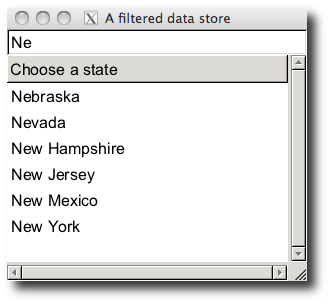
\includegraphics[width=.45\textwidth]{ex-RGtk2-filtered}
  \caption{Example of a data store filtered by values typed into a
    text-entry widget.}
  \label{fig:RGtk2-filtered}
\end{figure}

First, we create a data frame. The
\code{visible} column will be added to the \code{rGtkDataFrame}
instance to adjust the visible rows.
\begin{Schunk}
\begin{Sinput}
 df <- data.frame(state.name)
 df$visible <- rep(TRUE, nrow(df))
 store <- rGtkDataFrame(df)
\end{Sinput}
\end{Schunk}

The filtered store needs to have the column specified that contains
the logical values; in this example, it is the last column.
\begin{Schunk}
\begin{Sinput}
 filteredStore <- store$filter()
 filteredStore$setVisibleColumn(ncol(df)-1)      # offset
 view <- gtkTreeView(filteredStore)
\end{Sinput}
\end{Schunk}

Next, we create a basic view of a single column:
\begin{Schunk}
\begin{Sinput}
 view$insertColumnWithAttributes(0, "Col", 
                  gtkCellRendererText(), text = 0)
\end{Sinput}
\end{Schunk}

An entry widget will be used to control the filtering. In the
callback, we adjust the \code{visible} column of the
\code{rGtkDataFrame} instance to reflect the rows to be shown. When
\code{val} is an empty string, the result of \function{grepl} is 
\code{TRUE}, so all rows will be shown.
\begin{Schunk}
\begin{Sinput}
 e <- gtkEntry()
 gSignalConnect(e, "changed", function(w, data) {
   pattern <- w$getText()
   df <- data$getModel()
   values <- df[, "state.name"]
   df[, "visible"] <- grepl(pattern, values)
 }, data=filteredStore)
\end{Sinput}
\end{Schunk}


Figure~\ref{fig:RGtk2-filtered} shows the two widgets placed within a
simple GUI.
\end{example}

\subsection{Cell renderer details}
\label{sec:RGtk2:cellrenderers}

The values in a tree model are rendered in a rectangular cell by the
derivatives of \class{GtkCellRenderer}. Cell renderers are
interactive, in that they also manage editing and activation of cells.

A cell renderer is independent of any data model. Its rendering role
is limited to drawing into a specified rectangular region according to
its current property values. An object that implements the
\class{GtkCellLayout} interface, like \class{GtkTreeViewColumn} and
\class{GtkComboBox} (see Section~\ref{sec:RGtk2:mvc:combobox}),
associates a set of \emph{attributes} with a cell renderer. An
attribute is a link between an aesthetic property of a cell renderer
and a column in the data model. When the \class{GtkCellLayout} object
needs to render a particular cell, it configures the properties of the
renderer with the values from the current model row, according to the
attributes. Thus, the mapping from data to visualization depends on
the class of the renderer instance, its explicit property settings,
and the attributes associated with the renderer in the cell layout.

For example, to render text, a \class{GtkCellRendererText} is
appropriate. The \code{text} property is usually linked via an
attribute to a text column in the model, as the text would vary from
row to row. However, the background color (the \code{cell-background}
property) might be common to all rows in the column and thus is set
explicitly, without use of an attribute:
\begin{Schunk}
\begin{Sinput}
 renderer <- gtkCellRendererText()
 renderer['cell-background'] <- "gray"
\end{Sinput}
\end{Schunk}

The base class \class{GtkCellRenderer} defines a number of properties
that are common to all rendering tasks. The \code{xalign} and
\code{yalign} properties specify the alignment, i.e., how to position
the rendered region when it does not fill the entire cell. The
\code{cell-background} property indicates the color for the entire
cell background.

The rest of this section describes each type of cell renderer, as well
as some advanced features.

%% text/ numbers
\paragraph{Text cell renderers}

\constructor{GtkCellRendererText} displays text and numeric
values. Numeric values in the model are shown as strings.  The most
important property is \code{text}, the actual text that is
displayed. Other properties control the display of the text, such as
the font \code{family} and \code{size}, the \code{foreground} and
\code{background} colors, and whether to \code{ellipsize} or
\code{wrap} the text if there is not enough space for display. There
are several other attributes that can changed.  For example, we
display right-aligned text in a Helvetica font:
\begin{Schunk}
\begin{Sinput}
 cr <- gtkCellRendererText()
 cr['xalign'] <- 1                    # default 0.5 = centered
 cr['family'] <- "Helvetica"  
\end{Sinput}
\end{Schunk}

When an attribute links the \code{text} property to a numeric column
in the model, the property system automatically converts the number to
its string representation. This occurs according to the same logic
that \R\/ follows to print numeric values, so options like
\code{scipen} and \code{digits} are considered. See the ``Overriding
attribute mappings'' paragraph below for further customization.

\paragraph{Editable cells} When the \code{editable} property of a text
cell (or \code{activatable} property of a toggle cell) is set to
\code{TRUE}, then the cell contents can be changed. This allows the
user to make changes to the underlying model through the GUI. Although
the view automatically reflects changes made to the model, the reverse
is not true. A callback must be assigned to the \code{editable}
(\code{toggled}) signal for the cell renderer to implement the
change. The callback for the \qcode{edited} signal has arguments
\code{renderer}, \code{path} for the path of the selected row (as a
string), and \code{new.text} containing the value of the edited text
as a string. The tree view object and the column index are not passed
to the callback, unless one uses a closure or user data.
For example, here is how one can update an \code{RGtkDataFrame} model
from within the callback:
\begin{Schunk}
\begin{Sinput}
 cr['editable'] <- TRUE
 ID <- gSignalConnect(cr, "edited", 
 f=function(cr, path, newtext, user.data) {
   i <- as.numeric(path) + 1
   j <- user.data$column
   model <- user.data$model
   model[i, j] <- newtext
 }, data=list(model=store, column=1))
\end{Sinput}
\end{Schunk}
% 
Before using editable cells to create a data frame editor, one should
see if the editor provided by the \function{gtkDfEdit} in the
\pkg{RGtk2Extras} package satisfies the requirements.

Users may expect that once a cell is edited, the next cell is then set
up to be edited. In order to do this, one must advance the cursor and
activate editing of the next cell. For \class{GtkTreeView}, this is
implemented by the \method{setCursor}{gtkTreeView} method. The
\code{path} argument takes a tree path instance, the \code{column}
argument should be a tree view column object, and the flag
\code{start.editing} indicates whether to initiate editing.

\begin{example}{Using a table to gather arguments}{ex:RGtk2-options-in-table}

This example shows one way to gather arguments or options using an
editable cell in a table, rather than a separate text entry
widget. Tables can provide compact entry areas in a familiar
interface.

For this example we collect values for arguments to the
\function{title} function. We first create a data frame with the
argument name and default value, along with some additional values:
\begin{Schunk}
\begin{Sinput}
 opts <- c("main","sub","xlab","ylab", "line","outer")
 df <- data.frame(option=opts,
            value=c("","","","","0","FALSE"),
            class=c(rep("character", 4), "integer", "logical"),
            edit_color=rep("gray95", 6),
            dirty = rep(FALSE, 6),
            stringsAsFactors=FALSE)
\end{Sinput}
\end{Schunk}
%
Unfortunately, we need to coerce the default values to character, in
order to store them in a single column. We preserve the class in the
\code{class} column, for coercion later. The \code{edit\_color} and
\code{dirty} columns are related to editing and explained later.
%

Now we create our model 
\begin{Schunk}
\begin{Sinput}
 m <- rGtkDataFrame(df)
 v <- gtkTreeView(m)
\end{Sinput}
\end{Schunk}
%
and configure the first column
\begin{Schunk}
\begin{Sinput}
 cr <- gtkCellRendererText()
 cr['background'] <- 'gray80'
 v$insertColumnWithAttributes(position=-1,
                              title="Option",
                              cell=cr,
                              text=1 - 1)
\end{Sinput}
\begin{Soutput}
[1] 1
\end{Soutput}
\end{Schunk}
%
The first column has a special background color which we specify
below, which indicates that the cells are not editable.
The second column is editable and has a background color that is
state dependent and indicates if a cell has been edited:
\begin{Schunk}
\begin{Sinput}
 cr <- gtkCellRendererText()
 cr['editable'] <- TRUE
 v$insertColumnWithAttributes(position = -1,
                              title = "Value",
                              cell = cr,
                              text = 2 - 1,
                              background = 4 - 1
                              )
\end{Sinput}
\end{Schunk}

To attach the view to the model, we connect the cell renderer to the
\signal{edited} signal. Here we use the \code{class} value to format
the text and then set the background color and \code{dirty} flag of the
entry. The latter allows one to easily find the values which were edited.
\begin{Schunk}
\begin{Sinput}
 gSignalConnect(cr, "edited", function(cr, path, new.text, 
                                       user.data) {
   m <- user.data$model
   i <- as.numeric(path) + 1; j <- user.data$column
   m[i,j] <- as(as(new.text, m[i, 'class']), "character")   
   m[i, 'dirty'] <- TRUE                     # mark dirty
   m[i, 'edit_color'] <- 'gray70'            # change color
 }, data=list(model=m, column=2))
\end{Sinput}
\end{Schunk}

A simple window displays our GUI.
\begin{Schunk}
\begin{Sinput}
 w <- gtkWindow(show=FALSE)
 w['title'] <- "Option editor"
 w$setSizeRequest(300,500)
 sw <- gtkScrolledWindow()
 w$add(sw)
 sw$add(v)
 w$show()
\end{Sinput}
\end{Schunk}

Implementing this into a GUI requires writing a function to map the
model values into the appropriate call to the \function{title} function. The
\code{dirty} flag makes this easy, but this is a task we do not pursue
here. Instead we add a bit of extra detail by providing a tooltip.

%% ML: This section makes me uncomfortable, since it's relying on very
%% volatile code. Internal routines from a package in active
%% development, which in turn rely on undocumented and internal
%% features of R.
\paragraph{Tooltips}
For this example, our function has built-in documentation. Below we
use the \pkg{helpr} function to extract the description for
each of the arguments. We leave this in a list, \code{descs}, for later
lookup.  
\begin{Schunk}
\begin{Sinput}
 require(helpr, quietly=TRUE)
 package <- "graphics"; topic <- "title"
 rd <- helpr:::parse_help(helpr:::pkg_topic(package, topic), 
                          package = package)
 descs <- rd$params$args
 names(descs) <- sapply(descs, function(i) i$param)
\end{Sinput}
\end{Schunk}

It is important to note that we are calling internal routines of a
package still under active development, which in turn relies on
volatile features of R. The purpose of this example is only to
demonstrate tooltips on a tree view.  For many widgets, adding a
tooltip is as easy as calling
\method{setTooltipText}{GtkWidget}. However, it is more complicated in
a tree view, as each cell should get a different tip.  To add tooltips
to the tree view we first indicate that we want tooltips, then connect
to the \signal{query-tooltip} signal to implement the tooltip:
\begin{Schunk}
\begin{Sinput}
 v["has-tooltip"] <- TRUE
 gSignalConnect(v, "query-tooltip", 
        function(w, x, y, key_mode, tooltip, user.data) {
          out <- w$getTooltipContext(x, y, key_mode)
          if(out$retval) {
            m <- w$getModel()
            i <- as.numeric(out$path$toString()) + 1
            val <- m[i, "option"]
            txt <- descs[[val]]$desc
            txt <- gsub("code>","b>", txt)  # no code in PANGO
            tooltip$setMarkup(txt)
            TRUE
          } else {
            FALSE                           # no tooltip
          }
        })
\end{Sinput}
\end{Schunk}
%
Within this callback we check if we have the appropriate context (we
are in a row), then, if so, use the path to find the description to
set in the tooltip. The descriptions use HTML for markup, but the
tooltip only uses PANGO. As the \code{code} tag is not PANGO, we
change to a bold tag using \function{gsub}.
\end{example}

%% XXX JV Add in an editable table example here, mention
%% RGtk2Extras:::gtkDfEdit

%% perhaps could be adapted to demonstrate the above
% \begin{example}{A basic usage of displaying a data frame using a tree view}{ex:RGtk2-minimal-rGtkDataFrame}
%   \SweaveInput{ex-RGtk2-minimal-rGtkDataFrame}
% \end{example}

%% combo
\paragraph{Combo and spin cell renderers}

\class{GtkCellRendererCombo} and \class{GtkCellRendererSpin} allow
editing a text cell with a combo box or spin button,
respectively. Populating the combo box menu requires specifying two
properties: \code{model} and \code{text-column}. The menu items are
retrieved from the \class{GtkTreeModel} given by \code{model} at the
column index given by \code{text-column}.  If \code{has-entry} is
\code{TRUE}, a combo box entry is displayed.
\begin{Schunk}
\begin{Sinput}
 cr <- gtkCellRendererCombo()
 store <- rGtkDataFrame(state.name)
 cr['model'] <- store
 cr['text-column'] <- 0
 cr['editable'] <- TRUE                  # needed
\end{Sinput}
\end{Schunk}
%
The spin button editor is configured by setting a
\class{GtkAdjustment} on the \code{adjustment} property.


%% pixbuf
\paragraph{Pixbuf cell renderers}

To display an image in a cell, \class{GtkCellRendererPixbuf} is
appropriate. The image is specified through one of these properties:
\code{stock-id}, a stock identifier; \code{icon-name}, the name of a
themed icon; or \code{pixbuf}, an actual \code{GdkPixbuf} object,
holding an image in memory. Using a \class{list}, one can store a
\class{GdkPixbuf} in a \class{data.frame}, and thus an
\class{RGtkDataFrame}. This is demonstrated in the next example.

% <<rgtk2-mvc-pixbuf-in-df>>=
% library(RGtk2)
% apple <- gdkPixbuf(filename = imagefile("apple-red.png"))[[1]]
% floppy <- gdkPixbuf(filename = imagefile("floppybuddy.gif"))[[1]]
% logo <- gdkPixbuf(filename = imagefile("rgtk-logo.gif"))[[1]]
% rdf <- rGtkDataFrame(data.frame(image = I(list(apple, floppy, logo))))
% view <- gtkTreeView(rdf)
% view$insertColumnWithAttributes(0, "image", gtkCellRendererPixbuf(), pixbuf = 0)
% win <- gtkWindow()
% win$add(view)
% @


%% JV redid, a tighter programmed
\begin{example}{A variable selection widget}{ex:RGtk2-variable-selection}

%% ML: John, I changed this to explicitly treat the selected and
%% unselected widgets, instead of looping over the pairs. It just
%% seemed like looping over two discrete things added unnecessary
%% complexity. Sure, the code is a little more verbose now, but it's
%% probably more readable. The other big change was using one model
%% and a custom filter.

This example shows how to create a GUI for selecting variables from a
data frame. The GUI is based on two lists. The left one indicates the
variables that can be selected, and the right shows the variables that
have been selected. An icon, indicating the variable type, is placed
next to the variable name. A similar mechanism is part of the SPSS
model specification GUI of
Figure~\ref{fig:GUI:spss-11-term-selection}. For illustration purposes
we use the \code{Cars93} data set.
\begin{Schunk}
\begin{Sinput}
 df <- get(data(Cars93, package="MASS"))
\end{Sinput}
\end{Schunk}

First, we render an icon for each variable.  The \code{make\_icon}
function from the \pkg{ProgGUIinR} package creates an icon as a
\pkg{grid} object, which we render with \pkg{cairoDevice}:
% 
\begin{Schunk}
\begin{Sinput}
 make_icon_pixmap <- function(x, ...) {
   require(grid); require(cairoDevice)
   pixmap <- gdkPixmap(drawable=NULL, width=16, height=16, 
   depth=24)
   asCairoDevice(pixmap)
   grid.newpage()
   grid.draw(make_icon(x))
   dev.off()
   gdkPixbufGetFromDrawable(NULL, pixmap, NULL, 0,0,0,0,-1,-1)
 }
\end{Sinput}
\end{Schunk}

The two list views are based on the same underlying data model, which
contains three columns: the variable name, the icon, and
whether the variable has been selected. We construct the corresponding
data frame and wrap it in a \class{RGtkDataFrame}:
\begin{Schunk}
\begin{Sinput}
 mdf <- data.frame(Variables = I(sort(names(df))),
                   icon = I(sapply(df, make_icon_pixmap)),
                   selected = rep(FALSE, ncol(df)))
 model <- rGtkDataFrame(mdf)
\end{Sinput}
\end{Schunk}

The first view shows only unselected variables, while the other is
limited to selected variables. Thus, each view will be based on a
different filter:
\begin{Schunk}
\begin{Sinput}
 selectedFilter <- model$filter()
 selectedFilter$setVisibleColumn(2)
 unselectedFilter <- model$filter()
 unselectedFilter$setVisibleFunc(function(model, iter) {
   !model$get(iter, 2)[[1]]
 })
\end{Sinput}
\end{Schunk}
%
The selected filter is relatively easy to define, using
\code{selected} as the visible column. For the unselected filter, we
need to define a custom visible function that inverts the
\code{selected} column.

Next, we create a view for each filter:
\begin{Schunk}
\begin{Sinput}
 unselectedView <- gtkTreeView(unselectedFilter)
 selectedView <- gtkTreeView(selectedFilter)
 unselectedView$getSelection()$setMode('multiple')
 selectedView$getSelection()$setMode('multiple')
\end{Sinput}
\end{Schunk}

Each cell needs to display both an icon and a label.  This is achieved
by packing two cell renderers into the column:
\begin{Schunk}
\begin{Sinput}
 make_view_column <- function() {
   vc <- gtkTreeViewColumn()
   vc$setTitle("Variable")
   cr <- gtkCellRendererPixbuf()
   vc$packStart(cr)
   vc$addAttribute(cr, "pixbuf", 1)
   cr <- gtkCellRendererText()
   vc$packStart(cr)
   vc$addAttribute(cr, "text", 0)
   vc
 }
 unselectedView$insertColumn(make_view_column(), 0)
 selectedView$insertColumn(make_view_column(), 0)
\end{Sinput}
\end{Schunk}

For later use we extend the API for a tree view -- one method to find
the selected indices ($1$-based) and one to indicate if there is a
selection: 
\begin{Schunk}
\begin{Sinput}
 gtkTreeViewSelectedIndices <- function(object) {
   paths <- object$getSelection()$getSelectedRows()$retval
   out <- sapply(paths, function(i) {
     model <- object$getModel()          # Filtered!
     model$convertPathToChildPath(i)$toString()
   })
   if(length(out) == 0)
     integer(0)
   else
     as.numeric(out) + 1                             # 1-based
 }
 #
 gtkTreeViewHasSelection <-
   function(obj) length(obj$selectedIndices()) > 0
\end{Sinput}
\end{Schunk}

Now we create the buttons and connect to the \code{clicked}
signal. The handler moves the selected values to the other list by
toggling the \code{selected} variable:
\begin{Schunk}
\begin{Sinput}
 selectButton <- gtkButton(">")
 unselectButton <- gtkButton("<")
 toggleSelectionOnClick <- function(button, view) {
   gSignalConnect(button, "clicked", function (x) {
     ind <- view$selectedIndices()
     model[ind, "selected"] <- !model[ind, "selected"]
   })
 }
 toggleSelectionOnClick(selectButton, unselectedView)
 toggleSelectionOnClick(unselectButton, selectedView)
\end{Sinput}
\end{Schunk}
%
We only want our buttons sensitive if there is a possible move. This
is determined by the presence of a selection:
\begin{Schunk}
\begin{Sinput}
 selectButton['sensitive'] <- FALSE
 unselectButton['sensitive'] <- FALSE
 trackSelection <- function(button, view)
   gSignalConnect(view$getSelection(), "changed", 
     function(x) button['sensitive'] <- view$hasSelection())
 trackSelection(selectButton, unselectedView)
 trackSelection(unselectButton, selectedView)
\end{Sinput}
\end{Schunk}

We now layout our GUI using a horizontal box, into which is packed the
views and a box holding the selection buttons. The views
will be scrollable, so we place them in scrolled windows:
\begin{Schunk}
\begin{Sinput}
 w <- gtkWindow(show=FALSE)
 w$setDefaultSize(600, 400)
 g <- gtkHBox()
 w$add(g)
 selectedScroll <- gtkScrolledWindow()
 selectedScroll$add(selectedView)
 selectedScroll$setPolicy("automatic", "automatic")
 unselectedScroll <- gtkScrolledWindow()
 unselectedScroll$add(unselectedView)
 unselectedScroll$setPolicy("automatic", "automatic")
 buttonBox <- gtkVBox()
 centeredBox <- gtkVBox()
 buttonBox$packStart(centeredBox, expand = TRUE, fill = FALSE)
 centeredBox$setSpacing(12)
 centeredBox$packStart(selectButton, expand = FALSE)
 centeredBox$packStart(unselectButton, expand = FALSE)
 g$packStart(unselectedScroll, expand=TRUE)
 g$packStart(buttonBox, expand=FALSE)
 g$packStart(selectedScroll, expand=TRUE)
\end{Sinput}
\end{Schunk}

Finally, we show the top-level window:
\begin{Schunk}
\begin{Sinput}
 w$show()
\end{Sinput}
\end{Schunk}


\end{example}

% %% ping pong
% \begin{example}{A widget for variable selection}{ex:RGtk2-pingpong}
%   \SweaveInput{ex-RGtk2-pingpong}
% \end{example}

\paragraph{Toggle cell renderers}

Binary data can be represented by a toggle. The
\constructor{gtkCellRendererToggle} will create a check box in the
cell that will appear checked if the \code{active} property is
\code{TRUE}. If an attribute is defined for the property, then changes
in the model will be reflected in the view. More work is required to
modify the model in response to user interaction with the view. The
\code{activatable} attribute for the cell must be \code{TRUE} in order
for it to receive user input. The programmer then needs to connect to the
\signal{toggled} to update the model in response to changes in the
active state.
\begin{Schunk}
\begin{Sinput}
 cr <- gtkCellRendererToggle()
 cr['activatable'] <- TRUE             # cell can be activated
 cr['active'] <- TRUE
 gSignalConnect(cr, "toggled", function(w, path) {
   model$active[as.numeric(path) + 1] <- w['active']
 })
\end{Sinput}
\end{Schunk}

To render the toggle as a radio button instead of a check box, set the
\code{radio} property to \code{TRUE}. Again, the programmer is
responsible for implementing the radio button logic via the
\code{toggled} signal.

\begin{example}{Displaying a check box column in a tree
    view}{ex:RGtk2-add-toggle-to-df}
This example demonstrates the construction of a GUI for selecting one
or more rows from a data frame. We will display a list of the installed
packages that can be upgraded from CRAN, although this code is
trivially generalizable to any list of choices. The user selects a row
by clicking on a 
check box produced by a toggle cell renderer.


To get the installed packages that can be upgraded, we use some of the
functions provided by the  \pkg{utils} package.
\begin{Schunk}
\begin{Sinput}
 d <- old.packages()[,c("Package", "Installed", "ReposVer")]
 d <- as.data.frame(d)
\end{Sinput}
\end{Schunk}


This function will be called on the selected rows. Here, we simply
call \function{install.packages} to update the selected packages.
\begin{Schunk}
\begin{Sinput}
 doUpdate <- function(d)  install.packages(d$Package)
\end{Sinput}
\end{Schunk}

To display the data frame, we first append a column to the data frame
to store the selection information and then create a corresponding
\class{RGtkDataFrame}.
\begin{Schunk}
\begin{Sinput}
 n <- ncol(d)
 nms <- colnames(d)
 d$.toggle <- rep(FALSE, nrow(d))
 store <- rGtkDataFrame(d)
\end{Sinput}
\end{Schunk}

Our tree view shows each text column using a simple text cell renderer,
except for the first column that contains the check boxes for selection.
\begin{Schunk}
\begin{Sinput}
 view <- gtkTreeView()
 # add toggle
 cr <- gtkCellRendererToggle()
 view$insertColumnWithAttributes(0, "", cr, active = n)
 cr['activatable'] <- TRUE
 gSignalConnect(cr, "toggled", function(cr, path, user.data) {
   view <- user.data
   row <- as.numeric(path) + 1
   model <- view$getModel()
   n <- dim(model)[2]
   model[row, n] <- !model[row, n]
 }, data=view)
\end{Sinput}
\end{Schunk}

The text columns are added in one go:
\begin{Schunk}
\begin{Sinput}
 mapply(view$insertColumnWithAttributes, -1, nms, 
        list(gtkCellRendererText()), text = 1:n-1)
\end{Sinput}
\end{Schunk}
%
Finally, we connect the store to the model.
\begin{Schunk}
\begin{Sinput}
 view$setModel(store)
\end{Sinput}
\end{Schunk}
%
To allow the user to initiate the action, we create a button and
assign a callback. We pass in the view, rather than the model, in case
the model would be recreated by the \code{doUpdate} call. In a real
application, once a package is upgraded it would be removed from the
display.
\begin{Schunk}
\begin{Sinput}
 b <- gtkButton("Update packages")
 gSignalConnect(b, "clicked", function(w, data) {
   view <- data
   model <- view$getModel()
   n <- dim(model)[2]
   vals <- model[model[, n], -n, drop=FALSE]
   doUpdate(vals)
 }, data=view)
\end{Sinput}
\end{Schunk}


Our basic GUI places the view into a box container that also holds the
button to initiate the action.
\begin{Schunk}
\begin{Sinput}
 w <- gtkWindow(show=FALSE)
 w$setTitle("Installed packages that need upgrading")
 w$setSizeRequest(300, 300)
 g <- gtkVBox(); w$add(g)
 sw <- gtkScrolledWindow()
 g$packStart(sw, expand=TRUE, fill=TRUE)
 sw$add(view)
 sw$setPolicy("automatic", "automatic")
 g$packStart(b, expand=FALSE)
 w$show()
\end{Sinput}
\end{Schunk}
\end{example}

%% progress bars
\paragraph{Progress cell renderers}

To visually communicate progress within a cell, both progress bars and
spinner animations are supported. These modes correspond to
\class{GtkCellRendererProgress} and \class{GtkCellRendererSpinner},
respectively.

In the case of \class{GtkCellRendererProgress}, its \code{value}
property takes a value between $0$ and $100$ indicating the amount
finished, with a default value of $0$. Values out of this range will
be signaled by an error message.  For example,
\begin{Schunk}
\begin{Sinput}
 cr <- gtkCellRendererProgress()
 cr["value"] <- 50
\end{Sinput}
\end{Schunk}

For indicating progress in the absence of a definite end point,
\class{GtkCellRendererSpinner} is more appropriate. The spinner is
displayed when the \code{active} property is \code{TRUE}. Increment
the \code{pulse} property to drive the animation.

%% numbers
\paragraph{Overriding attribute mappings}

The default behavior for mapping model values to a renderer property
is simple: values are extracted from the model and passed directly to
the cell renderer property. If the data types are different, such as a
numeric value for a string property, the value is converted using
low-level routines defined by the property system. It is sometimes
desirable to override this mapping with more complex logic.

For example, conversion of numbers to strings is a non-trivial
task. Although the logic in the \R\/ print system often performs
acceptably, there is certainly room for customization. One example is
aligning floating point numbers by fixing the number of decimal
places. This could be done in the model (e.g., using
\function{sprintf} to format and coerce to character
data). Alternatively, one could preserve the integrity of the data and
perform the conversion during rendering. This requires intercepting
the model value before it is passed to the cell renderer. 

In the specific case \class{GtkTreeView}, it is possible to specify a
callback that overrides this step.  The callback, of type
\class{GtkTreeCellDataFunc}, is passed arguments for the tree view
column, the cell renderer, the model, an iterator pointing to the row
in the model and, optionally, an argument for user data. The function
is tasked with setting the appropriate attributes of the cell
renderer. For example, this callback would format floating point
numbers:
\begin{Schunk}
\begin{Sinput}
 func <- function(viewCol, cellRend, model, iter, data) {
   curVal <- model$getValue(iter, 0)$value
   fVal <- sprintf("%.3f", curVal)
   cellRend['text'] <- fVal
   cellRend['xalign'] <- 1
 }
\end{Sinput}
\end{Schunk}
%
The function then needs to be registered with a
\class{GtkTreeViewColumn} that is rendering a numeric column from the model:
\begin{Schunk}
\begin{Sinput}
 view <- gtkTreeView(rGtkDataFrame(data.frame(rnorm(100))))
 cr <- gtkCellRendererText()
 view$insertColumnWithAttributes(0, "numbers", cr, text = 0)
 vc <- view$getColumn(0)
 vc$setCellDataFunc(cr, func)
\end{Sinput}
\end{Schunk}
%
The last line is the key: calling
\method{setCellDataFunc}{GtkTreeViewColumn} registers our custom
formatting function with the view column.

One drawback with the use of such functions is that \R\/ code is
executed every time a cell is rendered. If performance matters,
consider pre-converting the data in the model or tweaking the
\code{options} in \R\/ for printing real numbers, namely \code{scipen}
and \code{digits}.

For customizing rendering further, and in the general case beyond
\class{GtkTreeView}, one could implement a new type of
\class{GtkCellRenderer}.  See Section~\ref{sec:gtk:extending-classes}
for more details on extending \GTK\/ classes.

%% This function will be set for the tree view column and illustrated in Example~\ref{ex:RGtk2:rGtk2DataFrame}.
%% editable cells 

\section{Display of hierarchical data}
\label{sec:RGtk2:mvc:GtkTreeStore}

Although the \code{RGtkDataFrame} model is a convenient implementation
of \class{GtkTreeModel}, it has its limitations. Primary among them is
its lack of support for hierarchical data. \GTK\/ implements
\class{GtkTreeModel} with \class{GtkListStore} and
\class{GtkTreeStore}, which respectively store non-hierarchical and
hierarchical tabular data. \class{GtkListStore} is a flat table,
while \class{GtkTreeStore} organizes the table into a hierarchy. Here,
we discuss \class{GtkTreeStore}.

\subsection{Loading hierarchical data}
  
%% ML: I'm pretty sure that RGtkDataFrame will support the same types
%% of values as GtkListStore. It's just a little tricky to get a
%% column of GdkPixbuf externalptr's into a data.frame. Much easier to
%% use a character vector and associate it with the stock.id property
%% of GtkCellRendererPixbuf, as long as the images are registered icons.

%% construction
A tree store is constructed using \constructor{gtkTreeStore}. The
column types are specified through a character vector at the time of
construction. The specification uses ``GTypes'' such as
\code{gchararray} for character data, \code{gboolean} for logical
data, \code{gint} for integer data, \code{gdouble} for numeric data,
and \code{GObject} for \GTK\/ objects, such as pixbufs.

\begin{example}{Defining a tree}{eg:RGtk2:tree-store}
  Below, we create a tree based on the \code{Cars93} dataset, where
  the car models are organized by manufacturer, i.e., each model row
  is the child of its manufacturer row:
\begin{Schunk}
\begin{Sinput}
 tstore <- gtkTreeStore("gchararray")
 by(Cars93, Cars93$Manufacturer, function(df) {
   piter <- tstore$append()              # parent
   tstore$setValue(piter$iter, column = 0, value = 
                   df$Manufacturer[1])
   sapply(df$Model, function(model) {
     sibiter <- tstore$append(parent = piter$iter) # child
     if (is.null(sibiter$retval)) 
       tstore$setValue(sibiter$iter, column = 0, value = model)
   })
 })
\end{Sinput}
\end{Schunk}
  To retrieve a value from the tree store using its path we have:
\begin{Schunk}
\begin{Sinput}
 iter <- tstore$getIterFromString("0:0")
 tstore$getValue(iter$iter, column = 0)$value
\end{Sinput}
\begin{Soutput}
[1] "Integra"
\end{Soutput}
\end{Schunk}
This obtains the first model from the first manufacturer.

\end{example}

As shown in this example, populating a tree store relies on two
functions: \method{append}{GtkTreeStore}, for appending rows, and
\method{setValue}{GtkTreeStore}, for setting row values. The iterator
to the parent row is passed to \method{append}{GtkTreeStore}. A parent
of \code{NULL}, the default, indicates that the row should be at the
top level. It would also be possible to insert rows using
\method{insert}{GtkTreeStore}, \method{insertBefore}{GtkTreeStore}, or
\method{insertAfter}{GtkTreeStore}. The
\method{setValue}{GtkTreeStore} method expects the row iterator and
the column index, $0$-based.

An entire row can be assigned through the \method{set}{gtkTreeStore}
method. The method uses positional arguments to specify the column and
the value. The column index appears as an even argument (say $2k$) and
the corresponding value in the odd argument (say $2k+1$).  Values are
returned by the \method{getValue}{gtkListStore} method, in a list with
component \code{value} storing the value.

Traversing a tree store is most easily achieved through the use of
\class{GtkTreeIter}, introduced previously in the context of flat
tables. Here we perform a depth-first traversal of our \code{Cars93}
model to obtain the model values: 
\begin{Schunk}
\begin{Sinput}
 iter <- tstore$getIterFirst()
 models <- NULL
 while(iter$retval) {
   child <- tstore$iterChildren(iter$iter)
   while(child$retval) {
     models <- c(models, tstore$get(child$iter, 0)[[1]])
     child$retval <- tstore$iterNext(child$iter)
   }
   iter$retval <- tstore$iterNext(iter$iter)
 }
\end{Sinput}
\end{Schunk}
%
The hierarchical structure introduces the method
\method{iterChildren}{GtkTreeModel} for obtaining an iterator to the
first child of a row. As with other methods returning iterators, the
return value is a list, with the \code{retval} component indicating
the validity of the iterator, stored in the \code{iter} component. The
method \method{iterParent}{GtkTreeModel} performs the reverse,
iterating from child to parent.

%% JV can add back in such a graphic. Took out for now.
% \begin{figure}
%   %% \centering
%   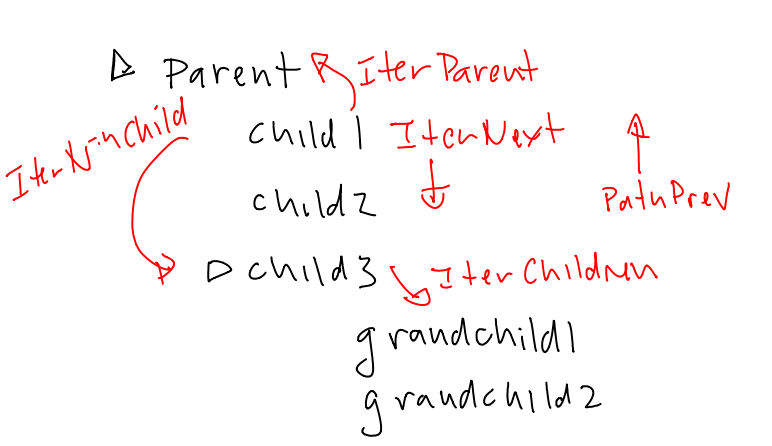
\includegraphics[width=.7\textwidth]{traverse-tree}
%   \caption{[REPLACEME!] Graphical illustration of the functions used
%     by iters to traverse a tree store. }
%   \label{fig:traverse-iter}
% \end{figure}

Rows within a store can be rearranged using several methods. Call
\method{swap}{gtkTreeStore} to swap rows referenced by their
iterators.  The methods \method{moveAfter}{gtkTreeStore} and
\method{moveBefore}{gtkTreeStore} move one row after or before
another, respectively.  The \method{reorder}{gtkTreeStore} method
totally reorders the rows under a specified parent given a vector of
row indices, like that returned by \function{order}.

%% clearing contents
Once added, rows may be removed using the
\method{remove}{gtkTreeStore} method. To remove every row, call the
\method{clear}{gtkTreeStore} method.

\subsection{Displaying data as a tree}
\label{sec:RGtk2:mvc:display-tree}

Once a hierarchical dataset has been loaded into a
\class{GtkTreeModel} implementation like \class{GtkTreeStore}, it can
be passed to a \class{GtkTreeView} widget for display as a
tree. Indeed, this is the same widget that displayed our flat data
frame in the previous section. As before, \class{GtkTreeView}
displays the \class{GtkTreeModel} as a table; however, it now adds
controls for expanding and collapsing nodes where rows are nested.

The user can click to expand or collapse a part of the tree. These
actions correspond to the signals \code{row-expanded} and
\code{row-collapsed}, respectively.

\begin{example}{A simple tree display}{eg:RGtk2-simple-tree}
Here, we demonstrate the application of \class{GtkTreeView} to the
display of hierarchical data. We will use the model constructed in
Example~\ref{eg:RGtk2:tree-store} from the \code{Cars93} dataset.  In
that example we defined a simple tree store from a data frame, with a
level for manufacturer and make for different cars. We refer to that
model by \code{tstore} below.



Now, we make a simple rectangular store for the model information with
the following:
\begin{Schunk}
\begin{Sinput}
 store <- rGtkDataFrame(Cars93[,"Model", drop=FALSE])
\end{Sinput}
\end{Schunk}

Creating a basic view is similar to that for rectangular data already presented:
\begin{Schunk}
\begin{Sinput}
 view <- gtkTreeView()
 view$insertColumnWithAttributes(0, "Make", 
            gtkCellRendererText(), text = 0)
\end{Sinput}
\begin{Soutput}
[1] 1
\end{Soutput}
\end{Schunk}


Finally, we illustrate that the same view can be used with either model:
\begin{Schunk}
\begin{Sinput}
 view$setModel(store)               # the rectangular store
 view$setModel(tstore)              # or the tree store
\end{Sinput}
\end{Schunk}
\end{example}

%% ## dynamic. 
%% JV: Is this too much? Perhaps leave for the package?
%% ML: Probably should move this to the package.
\begin{example}{Dynamically growing a tree}{eg:RGtk2:tree-dynamic}
This example uses a tree to explore an \R\/ list object, such as that
returned by one of \R's modeling functions.  As the depth of these
lists is not specified in advance, we use a dynamic approach to
that populates the tree store when a node is expanded and removes
nodes when their parent is collapsed.


We begin by defining our tree store and an accompanying tree
view. This example allows sorting, and so creates a sort proxy model:
\begin{Schunk}
\begin{Sinput}
 store <- gtkTreeStore(rep("gchararray", 2))
 sstore <- gtkTreeModelSort(store)
\end{Sinput}
\end{Schunk}

We create a root row:
\begin{Schunk}
\begin{Sinput}
 iter <- store$append(parent=NULL)$iter
 store$setValue(iter, column=0, "GlobalEnv")
 store$setValue(iter, column=1, "environment")
 iter <- store$append(parent=iter)
\end{Sinput}
\end{Schunk}
%
It is necessary to append an empty row to the root so that root
becomes expandable.

We now define the tree view and allow for multiple selection:
\begin{Schunk}
\begin{Sinput}
 view <- gtkTreeView(sstore)
 view$getSelection()$setMode("multiple")
\end{Sinput}
\end{Schunk}

The basic idea is to create child nodes when the parent is expanded
and to delete the children when the parent is collapsed. This relies
on the \code{row-expanded} and \code{row-collapsed} signals,
respectively. First, we define the expansion handler:
\begin{Schunk}
\begin{Sinput}
 gSignalConnect(view, signal = "row-expanded",
                f = function(view, iter, tpath, user.data) {
                  sortedModel <- view$getModel()
                  iter <- pathToIter(sortedModel, tpath)
                  path <- iterToRPath(sortedModel, iter)
                  children <- getChildren(path)
                  addChildren(store, children, parentIter=iter)
                  ## remove errant offspring, cf. addChildren
                  ci <- store$iterChildren(iter)
                  if(ci$retval) store$remove(ci$iter)
                })
\end{Sinput}
\end{Schunk}
%
The callback calls several helper functions to map the tree path to an
R object, get the child components of the object and add them to the
tree. The details are in the definitions of the helper functions.

The \function{pathToIter} function finds the iterator in the base tree
model for a tree path in the sorted proxy.
\begin{Schunk}
\begin{Sinput}
 pathToIter <- function(sstore, tpath) {
   store <- sstore$getModel()
   uspath <- sstore$convertPathToChildPath(tpath)
   store$getIter(uspath)$iter
 }
\end{Sinput}
\end{Schunk}

We now need to convert the iterator to an ``R path,'' which is made up
of the names of each component in the list. This function returns such
a path given an iterator:
\begin{Schunk}
\begin{Sinput}
 iterToRPath <- function(sstore, iter) {
   store <- sstore$getModel()
   indices <- store$getPath(iter)$getIndices()
   iter <- NULL
   path <- sapply(indices, function(i) {
     iter <<- store$iterNthChild(iter, i)$iter
     store$getValue(iter, 0)$value
   })
   return(path[-1])
 }
\end{Sinput}
\end{Schunk}

The \function{getChildren} function obtains the child components of a
given \R\/ object path. If the path is empty, the children are the
objects in the global environment, the root. The return value is a
\class{data.frame} with three columns: object name, object class and
whether the object is recursive.
\begin{Schunk}
\begin{Sinput}
 getChildren <- function(path=character(0)) {
   hasChildren <- function(obj) 
     (is.list(obj) || is.environment(obj)) && 
   !is.null(names(as.list(obj)))
   
   getType <- function(obj) head(class(obj), n=1)
 
   obj <- 
     if (!length(path)) {
       .GlobalEnv
     } else {
       x <- get(path[1], envir=.GlobalEnv)
       if(length(path) > 1)
         get(path[1], envir=.GlobalEnv)[[path[-1]]]
       else
         x
     }
 
   children <- as.list(obj)
   
   d <- data.frame(children = names(children),
                   class = sapply(children, getType),
                   offspring = sapply(children, hasChildren))
   
   ## filter out Gtk ones
   d[!grepl("^Gtk", d$class), ]
 }
\end{Sinput}
\end{Schunk}

The final step in the expansion handler is to add the children to the
tree store with the \function{addChildren} function.  Its one quirk is
the addition of a dummy child row when the item has children. This
makes the node expandable, i.e., the tree view draws an icon for the
user to click to request the expansion.
\begin{Schunk}
\begin{Sinput}
 addChildren <- function(store, children, parentIter = NULL) {
   if(nrow(children) == 0) 
     return(NULL)
   for(i in 1:nrow(children)) {
     iter <- store$append(parent=parentIter)$iter
     sapply(1:(ncol(children) - 1), function(j)              
            store$setValue(iter, column = j-1, children[i, j]))
     ## Add a branch if there are children
     if(children[i, "offspring"])
       store$append(parent=iter)
   }
 }
\end{Sinput}
\end{Schunk}

Next, we define a handler for the \code{row-collapsed} signal, which
has a similar signature as the \code{row-expanded} signal. The handler
removes the children of the newly collapsed node, so that we can add
them again when the node is expanded.
\begin{Schunk}
\begin{Sinput}
 gSignalConnect(view, signal = "row-collapsed",
        f = function(view, iter, tpath, user.data) {
          sortedModel <- view$getModel()
          iter <- pathToIter(sortedModel, tpath)
          n = store$iterNChildren(iter)
          if(n > 1) { ## n=1 gets removed when expanded
            for(i in 1:(n-1)) {
              child.iter <- store$iterChildren(iter)
              if(child.iter$retval)
                store$remove(child.iter$iter)
            }
          }
        })
\end{Sinput}
\end{Schunk}


Our last handler simply demonstrates the retrieval of an object when its
row is activated, i.e., double-clicked:
\begin{Schunk}
\begin{Sinput}
 gSignalConnect(view, signal = "row-activated",
        f = function(view, tpath, tcol) {
          sortedModel <- view$getModel()
          iter <- pathToIter(sortedModel, tpath)
          path <- iterToRPath(sortedModel, iter)
          sel <- view$getSelection()
          out <- sel$getSelectedRows()
          if(length(out) == 0) return(c()) # nothing
          vals <- c()
          for(i in out$retval) {  # multiple selections
            iter <- sortedModel$getIter(i)$iter
            newValue <- sortedModel$getValue(iter, 0)$value
            vals <- c(vals, newValue)
          }
          print(vals)  # [Replace this]
        })
\end{Sinput}
\end{Schunk}
 
To finish this example, we would need to populate the tree view with
columns and display the view in a window.



\end{example}
%% % ## mapes a list, shows how to update text view
% \SweaveInput{ex-RGtk2-tree-show}

\section{Model-based combo boxes}
\label{sec:RGtk2:mvc:combobox}

Basic combo box usage was discussed in
Section~\ref{sec:RGtk2:basic-combobox}; here we discuss the more
flexible and complex approach of using an explicit data model for
storing the menu items. The item data is tabular, although it is
limited to a single column. Thus, \class{GtkTreeModel} is again the
appropriate model, and \class{RGtkDataFrame} is usually the
implementation of choice.

To construct a \class{GtkComboBox} based on a user-created model, one
should pass the model to the constructor
\constructor{gtkComboBox}. This model may be changed or set through
the \method{setModel}{gtkComboBox} method and is returned by
\method{getModel}{gtkComboBox}. It remains to instruct the combo box
how to display one or more data columns in the menu. Like
\class{GtkTreeViewColumn}, \class{GtkComboBox} implements the
\class{GtkCellLayout} interface and thus delegates the rendering of
model values to \class{GtkCellRenderer} instances that are packed into
the combo box.

The \method{getActiveIter}{gtkComboBox} returns a list containing the iterator
pointing to the currently selected row in the model.  If no row has been
selected, the \code{retval} component of the list is \code{FALSE}.
The \method{setActiveIter}{gtkComboBox} sets the currently selected
item by iterator. As discussed previously, the
\method{getActive}{gtkComboBox} and \method{setActive}{gtkComboBox}
behave analogously with $0$-based indices.

As introduced in the previous chapter, the \class{GtkComboBoxEntry}
widget extends \class{GtkComboBox} to provide an entry widget for the
user to enter arbitrary values. To construct a combo box entry on top
of a tree model, one should pass the model, as well as the column
index that holds the textual item labels, to the
\constructor{gtkComboBoxEntry} constructor. It is not necessary to
create a cell renderer for displaying the text, as the entry depends
on having text labels and thus enforces their display. It is still
possible, of course, to add cell renderers for other model columns.

When a user selects a value with the mouse, the \code{changed} signal
is emitted. For combo box entry widgets, the \code{changed} signal
will also be emitted when a new value has been entered. To detect when
the user has finished entering text, one needs to retrieve the
underlying \class{GtkEntry} widget with \method{getChild}{GtkBin} and
connect to its \code{activate} signal.

\begin{example}{A combo box with memory}{eg:RGtk2-combobox-entry}

This example uses an editable combo box as an simple interface to the
\R\/ help system. Along the way, we record the number of times the
user searches for a page.

Our model for the combo box will be an \class{RGtkDataFrame} instance
with three columns: a function name, a string describing the
number of visits and an integer to record the number of visits. We
create the combo box with this model using the first column for the text:
\begin{Schunk}
\begin{Sinput}
 m <- rGtkDataFrame(data.frame(
              fname=character(0), visits=character(0), 
              novisits=integer(0), stringsAsFactors=FALSE))
 cb <- gtkComboBoxEntryNewWithModel(m, text.column=0)
\end{Sinput}
\end{Schunk}

It is not currently possible to put tooltip information on the drop
down elements of a combo box, as was done with a tree view. Instead,
we borrow from popular web browser interfaces and add textual
information about the number of visits to the drop down menu. This
requires us to pack in a new cell renderer to accompany the original
label provided by the \code{gtkComboBoxEntry} widget:
\begin{Schunk}
\begin{Sinput}
 cr <- gtkCellRendererText()
 cb$packStart(cr)
 cb$addAttribute(cr, "text", 1)
 cr['foreground'] <- "gray50"
 cr['ellipsize'] <- "end"
 cr['style'] <- "italic"
 cr['alignment'] <- "right"
\end{Sinput}
\end{Schunk}

%% JV: This first point seems like a misunderstanding on my part, but
%% I tried:
%% > m =rGtkDataFrame(data.frame(a=character(0), b=character(0), stringsAsFactors=FALSE))
%% > sapply(m[,], class)          a           b 
%% "character" "character" 
%% > m$appendRows(list(a="a", b="b"))
%% <pointer: 0x11eda4e30>
%% attr(,"interfaces")
%% [1] "GtkTreeModel"    "GtkTreeSortable"
%% attr(,"class")
%% [1] "RGtkDataFrame" "GObject"       "RGtkObject"   
%% > sapply(m[,], class)
%%        a        b 
%% "factor" "factor" 

%% ML: Just pass a data.frame to the appendRows function. The updating
%% dimensions comment was false. It was just a bug in RGtkDataFrame
%% that is now fixed in svn.

This helper function will be called each time a help page is
requested. It first updates the visit information, selects the
text for easier editing the next time round, then calls \function{help}.
\begin{Schunk}
\begin{Sinput}
 callHelpFunction <- function(cb, value) {
   model <- cb$getModel()
   ind <- match(value,model[,1, drop=TRUE])
   n <- model[ind, "novisits"] <- model[ind, "novisits"] + 1
   model[ind, "visits"] <- 
     sprintf(ngettext(n, "%s visit", "%s visits"), n)
   ## select for easier editing
   cb$getChild()$selectRegion(start=0,end=-1)
   help(value)
 }
 gSignalConnect(cb, "changed", f=function(w, ...) {
   if(cb$getActive() >= 0) {
     val <- w$getActiveText()
     callHelpFunction(w, val)
   }
 })
\end{Sinput}
\end{Schunk}
%

When the user enters a new value in the entry, we need to check if we
have previously accessed the item. If not, we add the value to our model.
\begin{Schunk}
\begin{Sinput}
 gSignalConnect(cb$getChild(), "activate", 
                f = function(cb, entry, ...) {
   val <- entry$getText()
   if(!any(val == cb$getModel()[,1, drop=TRUE])) {
     model <- cb$getModel()
     model$appendRows(data.frame(fname=val, visits="", novisits=0,
                                 stringsAsFactors = FALSE))
   }
   callHelpFunction(cb, val)
 }, data=cb, user.data.first=TRUE)
\end{Sinput}
\end{Schunk}

We place this in a minimal GUI with a label:
\begin{Schunk}
\begin{Sinput}
 w <- gtkWindow(show=FALSE)
 w['border-width'] <- 15
 g <- gtkHBox(); w$add(g)
 g$packStart(gtkLabel("Help on:"))
 g$packStart(cb, expand=TRUE, fill=TRUE)
 #
 w$show()
\end{Sinput}
\end{Schunk}

An alternative approach would be to use the completion support of
\class{GtkEntry}, presented next, but we leave that as an exercise to
the reader.

\end{example}


%% JV, moved this to the first intro of comoboboxes
% \begin{example}{Modifying the values in a combobox}{eg-RGtk2-combobox-dynamic}
%   \SweaveInput{ex-RGtk2-combobox-dynamic}
% \end{example}

%% JV this is in the menu section, not really needed here
% \begin{example}{A color selection widget}{eg:RGtk2:combobox}
%   \SweaveInput{ex-RGtk2-combobox}
% \end{example}


\section{Text entry widgets with completion}
\label{sec:RGtk2:entry-completion}

Often, the number of possible choices is too large to list in a combo
box. One example is a web-based search engine: the possible search
terms, while known and finite in number, are too numerous to list. The
auto-completing text entry has emerged as an alternative to a combo
box and might be described as a sort of dynamic combo box entry widget. 
When a user enters a string, partial matches to the string are
displayed in a menu that drops down from the entry. 

The \class{GtkEntryCompletion} object implements text completion in
\GTK. An instance is constructed with
\constructor{gtkEntryCompletion}. The underlying database is a
\class{GtkTreeModel}, like \class{RGtkDataFrame}, set via the
\method{setModel}{gtkEntryCompletion} method. To connect a
\class{GtkEntryCompletion} to an actual \class{GtkEntry} widget, call
the \method{setCompletion}{gtkEntry} method on \class{GtkEntry}.  The
\code{text-column} property specifies the column containing the
completion candidates. 

There are several properties that can be adjusted to tailor the
completion feature; we mention some of them. Setting the property
\code{inline-selection} to \code{TRUE} will place the top completion
suggestion to the entry inline as the completions are scrolled
through; \code{inline-completion} will add the common prefix
automatically to the entry widget; \code{popup-single-match} is a
logical indicating if a popup is displayed on a single match;
\code{minimum-key-length} takes an integer specifying the number of
characters needed in the entry before completion is checked (the
default is $1$).

By default, the rows in the data model that match the current value of
the entry widget in a case insensitive manner are displayed. This
matching function can be overridden by setting a new \R\/ function through
the \method{setMatchFunc}{gtkEntryCompletion} method. The signature of
this function is the completion object, the string from the entry
widget (lower case), an iterator pointing to a row in the model and
optionally user data that is passed through the \code{func.data}
argument of the \code{setMatchFunc} method. This callback should
return \code{TRUE} or \code{FALSE} depending on whether that row
should be displayed in the set of completions.

%% TODO: work this example into the above
\begin{example}{Text entry with completion}{eg:RGtk2:text-entry-comletion}
This example illustrates the steps to add completion to a text entry.


We create an entry with a completion database:
\begin{Schunk}
\begin{Sinput}
 entry <- gtkEntry()
 completion <- gtkEntryCompletion()
 entry$setCompletion(completion)
\end{Sinput}
\end{Schunk}

We will use an \code{RGtkDataFrame} instance for our completion model,
taking a convenient list of names for our example.  We set the model
and text column index on the completion object and then set some
properties to customize how the completion is handled:
\begin{Schunk}
\begin{Sinput}
 store <- rGtkDataFrame(state.name)
 completion$setModel(store)
 completion$setTextColumn(0)
 completion['inline-completion'] <- TRUE
 completion['popup-single-match'] <- FALSE
\end{Sinput}
\end{Schunk}

We wish for the text search to match against any part of a string, not
only the beginning, so we define our own match function:
\begin{Schunk}
\begin{Sinput}
 matchAnywhere <- function(comp, str, iter, user.data) {
   model <- comp$getModel()
   rowVal <- model$getValue(iter, 0)$value # column 0 in model
   
   str <- comp$getEntry()$getText()      # case sensitive
   grepl(str, rowVal)
 }
 completion$setMatchFunc(matchAnywhere)
\end{Sinput}
\end{Schunk}
%
We get the string from the entry widget, not the passed value, as the
latter has been standardized to lower case.




\end{example}

\section{Sharing Buffers Between Text Entries}
\label{sec:RGtk2:buffer-sharing}

As of \GTK\/ version $2.18$, multiple instances of \class{GtkEntry}
can synchronize their text through a shared buffer. Each entry obtains
its text from the same underlying model, a
\class{GtkEntryBuffer}. Here, we construct two entries, with a shared
buffer:
%% JVXXX needed to put in intial.chars, n.initial.chars into
%% constructor. No defaults, but could be
%% JV XXX does gtkEntry now have a buffer argument? I had to call
%% other constructor below to run
%% ML: The following should work eventually. I just have to re-run the code
%% generator.
\begin{Schunk}
\begin{Sinput}
 buffer <- gtkEntryBuffer()        
 entry1 <- gtkEntry(buffer = buffer)
 entry2 <- gtkEntry(buffer = buffer)
 entry1$setText("echo")
 entry2$getText()
\end{Sinput}
\end{Schunk}
%
The change of text in \qcode{entry1} has been reflected in
\qcode{entry2}.

\section{Text views} %% text buffer
\label{sec:RGtk2:textviews}

Multiline text areas are displayed through \class{GtkTextView}
instances. These provide a view of an accompanying
\class{GtkTextBuffer}, which is the model that stores the text and
other objects to be rendered. The view is responsible for the display
of the text in the buffer and has methods for adjusting tabs, margins,
indenting, etc. The text buffer stores the actual text, and its
methods are for adding and manipulating the text.

A text view is created with \constructor{gtkTextView}.  The underlying
text buffer can be passed to the constructor. Otherwise, a buffer is
automatically created.  This buffer is returned by the method
\method{getBuffer}{gtkTextView} and may be set with the
\method{setBuffer}{gtkTextView} method. Text views provide native
scrolling support and thus are easily added to a scrolled window
(Section~\ref{sec:RGtk2:scroll-windows}). 

\begin{example}{Basic \constructor{gtkTextView} usage}{eg:RGtk2:textview-basics}
  The steps to construct a text view consist of:
\begin{Schunk}
\begin{Sinput}
 w <- gtkWindow()
 w['border-width'] <- 15
 #
 tv <- gtkTextView()
 sw <- gtkScrolledWindow()
 sw$setPolicy("automatic", "automatic")
 #
 w$add(sw)
\end{Sinput}
\end{Schunk}
%
To set all the text in the buffer requires accessing the underlying
buffer:
\begin{Schunk}
\begin{Sinput}
 buffer <- tv$getBuffer()
 buffer$setText("Lorem ipsum dolor sit amet ...")
\end{Sinput}
\end{Schunk}

Manipulating the text requires an understanding of how positions are
referred to within the buffer (iterators or marks). As an indicator,
to get the contents of the buffer may be done as follows:
\begin{Schunk}
\begin{Sinput}
 start <- buffer$getStartIter()$iter    
 end <- buffer$getEndIter()$iter
 buffer$getText(start, end)
\end{Sinput}
\begin{Soutput}
[1] "Lorem ipsum dolor sit amet ..."
\end{Soutput}
\end{Schunk}

\end{example}

%% simple use -- replace, Append, insert at cursor

Text may be added programmatically through various methods of the text
buffer. The most basic \method{setText}{gtkTextBuffer}, which simply
replaces the current text, is shown in the example above. The method
\method{insertAtCursor}{gtkTextBuffer} will add the text to the buffer
at the current position of the cursor.  Other means are described in
the following sections.

By default, the text in a view is editable. This can be disabled
through the \property{editable}{QTextView} property. Typically, one
then sets the \property{cursor-visible}{QTextView} property to
\qcode{FALSE} so that the cursor is hidden:
\begin{Schunk}
\begin{Sinput}
 tv['editable'] <- FALSE
 tv['cursor-visible'] <- FALSE
\end{Sinput}
\end{Schunk}

%% properties: editable, ...
\paragraph{Formatting}
The text view supports several general formatting options. Automatic
line wrapping is enabled through \method{setWrapMode}{gtkTextView},
which takes values from \code{GtkWrapMode}: \qcode{none},
\qcode{char}, \qcode{word}, or \qcode{word\_char}. The justification
for the entire buffer is controlled by the \code{justification}
property which takes values of \qcode{left}, \qcode{right},
\qcode{center}, or \qcode{fill} from \code{GtkJustification}.  The
global value may be overridden for parts of the text buffer through
the use of text tags, see Section~\ref{sec:gtk-mvc-text-tags}. The
left and right margins are adjusted through the \code{left-margin} and
\code{right-margin} properties.

%% buffer - wide font
\paragraph{Fonts}
%% ML: do we need a general overview of Pango fonts?
The size and font can be globally set for a text view using the
\method{modifyFont}{gtkWidget} method. To set the font for specific
regions, use text tags, see Section~\ref{sec:gtk-mvc-text-tags}. The
font is specified as a Pango font description, which may be generated
from a string through \code{pangoFontDescriptionFromString}. These
strings may contain up to 3 parts: the first is a comma-separated list
of font families, the second a white-space separated list of style
options, and the third a size in points or pixels if the units ``px''
are included. A typical value might look like \code{"serif, monospace
  bold italic condensed 16"}. The various style options are enumerated
in \code{PangoStyle}, \code{PangoVariant}, \code{PangoWeight},
\code{PangoStretch}, and \code{PangoGravity}. The help page for
\code{PangoFontDescription} contains more information.

%% ML: stuff that could be described: automatic scrolling, and mapping
%% locations to text iterators. Already mentioned in the example though.

\section{Text buffers}
\label{sec:RGtk2:text-buffers}

Text buffer properties include \code{text} for the stored text and
\code{has-selection} to indicate if text is currently selected in a
view. The buffer also tracks if it has been modified. This information
is available through the buffer \method{getModified}{gtkTextBuffer}
method, which returns \code{TRUE} if the buffer has changed. To clear
this state, such as when a buffer has been saved to disk, one can pass
\code{FALSE} to \method{setModified}{gtkTextBuffer}.

In order to do more with a text buffer, such as retrieve a selection,
or modify text attributes, one needs to become familiar with the two
mechanism for referencing text in a buffer: iterators and marks.  A
text iterator is an opaque, transient pointer to a region of text,
whereas a text mark specifies a location that remains valid across
buffer modifications.

\subsection{Iterators}

%% text iters. GetStartIterm GetEndIter, GetSelectionBounds
%% transient

%% An iterator
An \dfn{iterator} is a programming object used to traverse through
some data, such as a text buffer or table of values. Iterators are
typically transient, in the sense that they are invalidated when their
source is modified. An iterator is often updated by reference,
behavior that is atypical in \R\/ programming.  In \GTK{} a \dfn{text
  iterator} is the primary means of specifying a position in a buffer.

%% methods to return an iterator
Several methods of the text buffer return iterators marking positions
in the buffer.  Iterators are returned as lists with two components:
\code{iter}, which represents the actual C iterator object, and
\code{retval}, a logical value indicating whether the iterator is
valid.  The beginning and end of the buffer are returned by the
methods \method{getStartIter}{gtkTextBuffer} and
\method{getEndIter}{gtkTextBuffer}. Both of these iterators are
returned together in a list by the method
\method{getBounds}{gtkTextBuffer}.  For example:
\begin{Schunk}
\begin{Sinput}
 bounds <- buffer$getBounds()
 bounds
\end{Sinput}
\begin{Soutput}
$retval
NULL

$start
<pointer: 0x103b28d90>
attr(,"interfaces")
character(0)
attr(,"class")
[1] "GtkTextIter" "GBoxed"      "RGtkObject" 

$end
<pointer: 0x1057ac330>
attr(,"interfaces")
character(0)
attr(,"class")
[1] "GtkTextIter" "GBoxed"      "RGtkObject" 
\end{Soutput}
\end{Schunk}
%
%% JV in the following I had to change bounds$start$iter to just
%% bounds$start. Not sure if this has changed in the newer RGtk2 -- I
%% had trouble installing the svn version due to a missing cairo
%% function. I'm stuck for now with the 2.18 from att.research.com package
The current selection is returned by the method
\method{getSelectionBounds}{gtkTextBuffer}, as a list of the same
structure. If there is no selection, then the component \code{retval}
will be \code{FALSE}, otherwise it is \code{TRUE}.

One can also obtain an iterator for a specific position in a
document. The method \method{getIterAtLine}{gtkTextBuffer} will return an
iterator pointing to the start of the line, which is specified by
$0$-based line number. The method
\method{getIterAtLineOffset}{gtkTextBuffer} has an additional argument
to specify the offset for a given line. An offset counts the number of
individual characters and keeps track of the fact that the text
encoding, UTF-8, may use more than one byte per character. For
example, we might request the seventh character of the first line:
\begin{Schunk}
\begin{Sinput}
 iter <- buffer$getIterAtLineOffset(0, 6)
 iter$iter$getChar()
\end{Sinput}
\begin{Soutput}
[1] 105
\end{Soutput}
\end{Schunk}
%
In addition to the text buffer, a text view also has the method
\method{getIterAtLocation}{gtkTreeView} to return the iterator
indicating the between-word space in the buffer closest to the point
specified in $x$-$y$ coordinates.

Once we obtain an iterator, we typically enter a loop which performs
some operation on the text at the iterator position and updates the
iterator with each iteration. This requires retrieving the text to
which an iterator refers. The character at the iterator position is
returned by \method{getChar}{GtkTextIter}. We obtain the first
character in the buffer:
\begin{Schunk}
\begin{Sinput}
 bounds$start$getChar()
\end{Sinput}
\begin{Soutput}
[1] 76
\end{Soutput}
\end{Schunk}
%
To obtain the text between two text
iterators, call the \method{getText}{GtkTextIter} method on the left
iterator, passing the right iterator as an argument:
\begin{Schunk}
\begin{Sinput}
 bounds$start$getText(bounds$end)
\end{Sinput}
\begin{Soutput}
[1] "Lorem ipsum dolor sit amet ..."
\end{Soutput}
\end{Schunk}
%
The \method{insert}{gtkTextBuffer} method will insert
text at a specified iterator:
\begin{Schunk}
\begin{Sinput}
 buffer$insert(bounds$start, "prefix")
\end{Sinput}
\end{Schunk}
%
The \method{delete}{gtkTextBuffer} method will delete the text between
two iterators.  An important observation is that we always pass the
actual iterator, i.e., the \code{iter} component of the list, to the
above methods. Passing the original list would not work.

%% iter methods
Next, we introduce the methods for updating an iterator. One can move
an iterator forward or backward, stopping a certain type of
landmark. Supported landmarks include characters (
\method{forwardChar}{gtkTextIter}, \method{forwardChars}{gtkTextIter},
\method{backwardChar}{gtkTextIter}, and
\method{backwordChars}{gtkTextIter}), words
(\method{forwardWordEnd}{gtkTextIter},
\method{backwardWordStart}{gtkTextIter}), and sentences
(\method{backwardSentenceStart}{gtkTextIter} and
\method{forwardSentenceEnd}{gtkTextIter}).  There are also various
methods, such as \method{insideWord}{gtkTextIter}, for determining the
textual context of the iterator. Example~\ref{eg:RGtk2-find-word}
shows how some of the above are used, in particular how these methods
update the iterator rather than return a new one.

\begin{example}{Finding the word that is clicked by the user}{eg:RGtk2-find-word}
  This example shows how one can find the iterator corresponding to a
  mouse click. We obtain the $X$ and $Y$ coordinates of the mouse
  button press event, find the corresponding iterator, and retrieve
  the surrounding word:
\begin{Schunk}
\begin{Sinput}
 ID <- gSignalConnect(tv, "button-press-event", 
                      f=function(w, e, ...) {
   siter <- w$getIterAtLocation(e$getX(), e$getY())$iter
   niter <- siter$copy()                 # need copy
   siter$backwardWordStart()
   niter$forwardWordEnd()
   val <- siter$getText(niter)
   print(val)                            # replace
   return(FALSE)                         # call next handler
 })
\end{Sinput}
\end{Schunk}
\end{example}

\subsection{Marks}

A text mark tracks a position in the document that is relative to
other text and is preserved across buffer modifications. One can think
of a mark as an invisible object stuck between two characters. A mark
corresponds to a specific position, like an iterator, except its
gravity sets it either to the left or right of the character. An
example is the text cursor, the position of which is represented by a
mark.

Marks are identified by name. We retrieve the mark for the
cursor, which is called \qcode{insert}:
\begin{Schunk}
\begin{Sinput}
 insert <- buffer$getMark("insert")
\end{Sinput}
\end{Schunk}

To access the text at a mark, we need to find the corresponding iterator:
\begin{Schunk}
\begin{Sinput}
 insertIter <- buffer$getIterAtMark(insert)$iter
 bounds$start$getText(insertIter)
\end{Sinput}
\begin{Soutput}
[1] "Lorem ipsum dolor sit amet ..."
\end{Soutput}
\end{Schunk}

Marks have a gravity of \qcode{left} or \qcode{right}, with
\qcode{right} being the default. If text is inserted at a mark with
right gravity, then the mark is moved to the end of the insertion. A
mark with left gravity would not be moved. This is intuitive if one
relates it to the behavior of the text cursor, which has right gravity:
\begin{Schunk}
\begin{Sinput}
 insertIter$getOffset()
\end{Sinput}
\begin{Soutput}
[1] 36
\end{Soutput}
\begin{Sinput}
 buffer$insert(insertIter, "insertion")
 buffer$getIterAtMark(insert)$iter$getOffset()
\end{Sinput}
\begin{Soutput}
[1] 45
\end{Soutput}
\end{Schunk}

A custom mark is created with its name, gravity and position. We
create one for the start of the document:
\begin{Schunk}
\begin{Sinput}
 mark <- buffer$createMark(mark.name = "start", 
                           where = buffer$getStartIter()$iter, 
                           left.gravity = TRUE)
\end{Sinput}
\end{Schunk}
%
By setting \argument{left.gravity}{gtkTextBufferCreateMark} to \qcode{TRUE}, the
iterator will not move when text is inserted.

%% tag Table
\subsection{Tags}
\label{sec:gtk-mvc-text-tags}

Tags are annotations placed on specific regions of a text buffer. To
create a tag, we call the \method{createTag}{gtkTextBuffer} method,
which takes an argument for each attribute to apply to the text. Here,
we create three tags: one for bold text, one for italicized text and
one for large text:
\begin{Schunk}
\begin{Sinput}
 tag.b <- buffer$createTag(tag.name="bold", 
                           weight=PangoWeight["bold"])
 tag.em <- buffer$createTag(tag.name="em", 
                            style=PangoStyle["italic"])
 tag.large <- buffer$createTag(tag.name="large", 
                               font="Serif normal 18")
\end{Sinput}
\end{Schunk}
%
Next, we associate the tags with one or more regions of text:
\begin{Schunk}
\begin{Sinput}
 iter <- buffer$getBounds()
 buffer$applyTag(tag.b, iter$start, iter$end)  # updates iters
 buffer$applyTagByName("em", iter$start, iter$end)
\end{Sinput}
\end{Schunk}

\subsection{Selection and the clipboard}

The selection is defined by the text buffer as the region between the
\qcode{insert} and \qcode{selection\_bound} marks. While we could
directly move the marks around, calling
\method{selectRange}{GtkTextBuffer} is more efficient and
convenient. Here, we select the first word:
\begin{Schunk}
\begin{Sinput}
 siter <- buffer$getStartIter()$iter
 eiter <- siter$copy(); eiter$forwardWordEnd()
\end{Sinput}
\begin{Soutput}
[1] TRUE
\end{Soutput}
\begin{Sinput}
 buffer$selectRange(siter, eiter)
\end{Sinput}
\end{Schunk}

\class{GtkTextBuffer} provides some convenience methods for
interaction with the clipboard: \method{copyCliboard}{gtkTextBuffer},
\method{cutClipboard}{gtkTextBuffer} and
\method{pasteClipboard}{gtkTextBuffer}. To use these, we first need a
clipboard object:
\begin{Schunk}
\begin{Sinput}
 cb <- gtkClipboardGet()
\end{Sinput}
\end{Schunk}
%
We can then, for example, copy the selected text (the first word) and
paste it at the end:
\begin{Schunk}
\begin{Sinput}
 buffer$copyClipboard(cb)
 buffer$pasteClipboard(cb, override.location = buffer$getEndIter()$iter, 
                       default.editable = TRUE)
\end{Sinput}
\end{Schunk}
%
The \argument{default.editable}{pasteClipboard} indicates that the
pasted text should be editable. If we had passed \qcode{NULL}, to the
\argument{override.location}{pasteClipboard} argument, the insertion
would have occured at the cursor.

% \begin{example}{Adding parentheses highlighting}{eg:RGtk2:paren-highlight}
%   \SweaveInput{ex-RGtk2-match-parentheses}
% \end{example}

%% insert images or widgets
\subsection{Inserting non-text items}

If desired, one can insert images and/or widgets into a text
buffer. The method \method{insertPixbuf}{gtkTextBuffer} will insert a
\class{GdkPixbuf} object. The buffer will count the image as a
character, although \method{getText}{gtkTextBuffer} will obviously not
return the image.

Arbitrary child widgets, like a button, can also be inserted. First,
one must create an anchor in the text buffer with
\method{createChildAnchor}{gtkTextBuffer}:
\begin{Schunk}
\begin{Sinput}
 anchor <- buffer$createChildAnchor(buffer$getEndIter()$iter)
\end{Sinput}
\end{Schunk}
%
To add the widget, we call the text view method
\method{addChildAtAnchor}{gtkTextView}:
\begin{Schunk}
\begin{Sinput}
 b <- gtkButton("click me")
 tv$addChildAtAnchor(b, anchor)
\end{Sinput}
\end{Schunk}

\begin{example}{A simple command line interface}{eg:RGtk2-command-line}
This example shows how to create a simple command line interface with
the text view widget. While few statistical applications will include
a command line widget, the example is familiar and shows several
different, but useful, aspects of the widget.

\begin{figure}
  \centering
  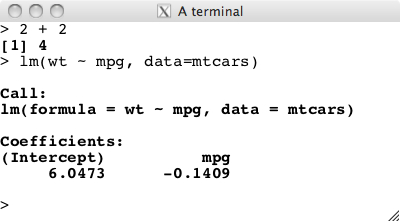
\includegraphics[width=.6\textwidth]{ex-RGtk2-terminal}
  \caption{A basic \R\/ terminal implemented using a \code{gtkTextView} widget.}
  \label{fig:RGtk2-terminal}
\end{figure}


We begin by defining our text view widget and retrieving its
buffer. We also specify a fixed-width font for the buffer.
\begin{Schunk}
\begin{Sinput}
 tv <- gtkTextView()
 tb <- tv$getBuffer()
 font <- pangoFontDescriptionFromString("Monospace")
 tv$modifyFont(font)                     # widget wide
\end{Sinput}
\end{Schunk}

We will use a few formatting tags, defined next. We do not need the tag
objects as variables in the workspace, as we refer to them later by name.
\begin{Schunk}
\begin{Sinput}
 tb$createTag(tag.name="cmdInput")
 tb$createTag(tag.name="cmdOutput", 
              weight=PangoWeight["bold"])
 tb$createTag(tag.name="cmdError", 
              weight=PangoStyle["italic"], foreground="red")
 tb$createTag(tag.name="uneditable", editable=FALSE)
\end{Sinput}
\end{Schunk}

We define a mark to indicate the beginning of a newly entered
command, and another mark tracks the end of the buffer:
\begin{Schunk}
\begin{Sinput}
 startCmd <- tb$createMark("startCmd", tb$getStartIter()$iter, 
                           left.gravity=TRUE)
 bufferEnd <- tb$createMark("bufferEnd", tb$getEndIter()$iter)
\end{Sinput}
\end{Schunk}

This helper function shows how to move the viewport to the end of the
buffer so that the command line is visibile:
\begin{Schunk}
\begin{Sinput}
 scrollViewport <- function(view, ...) {
   iter <- view$getBuffer()$getEndIter()$iter
   view$scrollToMark(bufferEnd, within.margin=0)
   return(FALSE)
 }
\end{Sinput}
\end{Schunk}

There are two types of prompts needed: one for entering a new command
and one for a continuation. This function adds either, depending on
its argument:
\begin{Schunk}
\begin{Sinput}
 addPrompt <- function(obj, prompt=c("prompt", "continue"),
                       setMark=TRUE) 
 {
   prompt <- match.arg(prompt)
   prompt <- getOption(prompt)
   
   endIter <- obj$getEndIter()
   obj$insert(endIter$iter, prompt)
   if(setMark)
     obj$moveMarkByName("startCmd", endIter$iter)
   obj$applyTagByName("uneditable", obj$getStartIter()$iter, 
                      obj$getEndIter()$iter)
 }
 addPrompt(tb) ## place an initial prompt
\end{Sinput}
\end{Schunk}

This helper method writes the output of a command to the text
buffer:
\begin{Schunk}
\begin{Sinput}
 addOutput <- function(obj, output, tagName="cmdOutput") {
   endIter <- obj$getEndIter()
   if(length(output) > 0) 
     sapply(output, function(i)  {
       obj$insertWithTagsByName(endIter$iter, i, tagName)
       obj$insert(endIter$iter, "\n", len=-1)
     })
 }
\end{Sinput}
\end{Schunk}
%
We arrange to truncate large outputs. By passing in the tag
name, we can specify whether this is normal output or an error
message.

This next function uses the \code{startCmd} mark and the end of the buffer
to extract the current command:
\begin{Schunk}
\begin{Sinput}
 findCMD <- function(obj) {
   endIter <- obj$getEndIter()
   startIter <- obj$getIterAtMark(startCmd)
   cmd <- obj$getText(startIter$iter, endIter$iter, TRUE)
   regex <- paste("\n[", getOption("continue"), "] ", sep = "")
   cmd <- unlist(strsplit(cmd, regex))
   cmd
 }
\end{Sinput}
\end{Schunk}
%
The \qcode{regex} is used to parse multi-line commands.

The following function takes the current command and evaluates it. It
uses a hack (involving \code{grep}) to distinguish between an
incomplete command and a true syntax error. 
\begin{Schunk}
\begin{Sinput}
 evalCMD <- function(tv, cmd) {
   tb <- tv$getBuffer()
   cmd <- paste(cmd, sep="\n")
   out <- try(parse(text=cmd), silent=TRUE)
   if(inherits(out, "try-error")) {
     if(length(grep("end", out))) {      # unexpected end 
       ## continue
       addPrompt(tb, "continue", setMark=FALSE)
     } else {
       ## error
       addOutput(tb, out, tagName = "cmdError")
     }
     scrollViewport(tv)
     return()
   }
   
   e <- parse(text = cmd)
   out <- capture.output(vis <- 
                  withVisible(try(eval(e, .GlobalEnv), TRUE)))
 
   addOutput(tb, out) 
   if (inherits(vis$value, "try-error"))
     addOutput(tb, vis$value, "cmdError")
   else if (vis$visible)
     addOutput(tb, capture.output(print(vis$value)))
   
   addPrompt(tb, "prompt", setMark=TRUE)
   scrollViewport(tv)  
 }
\end{Sinput}
\end{Schunk}

The \code{evalCMD} command is called when the \kbd{return} key is
pressed:
\begin{Schunk}
\begin{Sinput}
 gSignalConnect(tv, "key-release-event", f=function(w, e) {
   obj <- w$getBuffer()                  # w is textview
   keyval <- e$getKeyval()
   if(keyval == GDK_Return) {
     cmd <- findCMD(obj)                 # poss. character(0)
     if(length(cmd) && nchar(cmd) > 0)
       evalCMD(w, cmd)
   }
 })
\end{Sinput}
\end{Schunk}

%
%% ML: what is going on here? why is the signal commented out?
Finally, We connect \function{moveViewport} to the \code{changed}
signal of the text buffer, so that the view always scrolls to the
bottom when the contents of the buffer are modified:
% <<results=hide>>=
% gSignalConnect(tb, "changed", scrollViewport, tv, after = TRUE, 
%                user.data.first = TRUE)
% @ 

Figure~\ref{fig:RGtk2-terminal} shows the widget placed into a very
simple GUI.



\end{example}


% \begin{example}{Simple textview usage}{eg:RGtk2:simple-textview-usage}
%   \SweaveInput{ex-RGtk2-simple-textview}
% \end{example}





\chapter{RGtk2: Application Windows}
\label{sec:RGtk2-menus}
% Menus in RGtk2


In the traditional WIMP-style GUI, the user executes commands by
selecting items from a menu. In GUI terminology, such a command is
known as an \textit{action}. A GUI may provide more than one control
for executing a particular action. Menu Bars and toolbars are the two
most common widgets for organizing application-wide actions. An
application also needs to report its status in an unobtrusive
way. Thus, a typical application window contains, from top to bottom, 
a menu bar, a toolbar, a large application-specific region, and a
status bar.  In this chapter, we will introduce actions, menus,
toolbars and status bars and conclude by explaining the mechanisms in
\GTK\/ for conveniently defining and managing actions and associated
widgets in a large application.

\section{Actions}
\label{sec:RGtk2:actions}


\GTK\/ represents actions with the \class{GtkAction} class. A
\class{GtkAction} can be proxied by widgets like buttons in a
\class{GtkMenubar} or \class{GtkToolbar}.  The \constructor{gtkAction}
function is the constructor:
\begin{Schunk}
\begin{Sinput}
 a <- gtkAction(name="ok", label="_Ok", 
                tooltip="An OK button", stock.id="gtk-ok")
\end{Sinput}
\end{Schunk}
%
The constructor takes arguments \argument{name}{gtkAction} (to
programmatically refer to the action), \argument{label}{gtkAction}
(the displayed text), \argument{tooltip}{gtkAction}, and
\argument{stock.id}{gtkAction} (identifying a stock icon).  The
command associated with an action is implemented by a callback
connected to the \signal{activate} signal:
\begin{Schunk}
\begin{Sinput}
 gSignalConnect(a, "activate", f = function(w, data) {
   print(a$getName())                    # or some useful thing
 })
\end{Sinput}
\end{Schunk}

An action plays the role of a data model describing a command, while
widgets that implement the \class{GtkActivatable} interface are the
views and controllers. All buttons, menu items and tool items
implement \class{GtkActivatable} and thus may serve as action
proxies. Actions are connected to widgets through the method
\method{setRelatedAction}{gtkActivatable}:
\begin{Schunk}
\begin{Sinput}
 b <- gtkButton()
 b$setRelatedAction(a)
\end{Sinput}
\end{Schunk}
%
Certain aspects of a proxy widget are coordinated through the
action. This includes sensitivity and visibility, corresponding to the
\code{sensitive} and \code{visible} properties. By default, aesthetic
properties like the \code{label} and \code{stock-id} are also
inherited.

Often, the commands in an application have a natural grouping. It can
be convenient to coordinate the sensitivity and visibility of entire
groups of actions. \class{GtkActionGroup} represents a group of
actions. By convention, keyboard accelerators are organized by group,
and the accelerator for an action is usually specified upon insertion:
\begin{Schunk}
\begin{Sinput}
 group <- gtkActionGroup()
 group$addActionWithAccel(a, "<control>O")
\end{Sinput}
\end{Schunk}

In addition to the properties already introduced, an action may have a
shorter label for display in a toolbar (\code{short\_label}), and
hints for when to display its label (\code{is\_important}) and image
(\code{always\_show\_image}).

There is a special type of action that has a toggled state:
\class{GtkToggleAction}. The \code{active} property represents the
toggle. A further extension is \class{GtkRadioAction}, where the
toggled state is shared across a list of radio actions, via the
\code{group} property. Proxy widgets represent toggle and radio
actions with controls resembling check boxes and radio buttons,
respectively. Here, we create a toggle action for fullscreen mode:
\begin{Schunk}
\begin{Sinput}
 fullScreen <- gtkToggleAction("fullscreen", "Full screen", 
                               "Toggle full screen")
 gSignalConnect(fullScreen, "toggled", function(action) {
   if(fullScreen['active'])
     window$fullscreen()
   else
     window$unfullscreen()
 })
\end{Sinput}
\end{Schunk}
%
We connect to the \code{toggled} signal to respond to a change in the
action state.


\section{Menus}
\label{sec:RGtk2:menus}

A menu is a compact, hierarchically organized collection of buttons,
each of which may proxy an action. Menus listing window-level actions
are usually contained within a menu bar at the top of the window or
screen. Menus with options specific to a particular GUI element may
``popup'' when the user interacts with the element, such as by
clicking the right mouse button. Menu bars and popup menus may be
constructed by appending each menu item and submenu separately, as
illustrated below. For menus with more than a few items, we recommend
the strategies described in Section~\ref{sec:RGtk2:UIManager}.

\subsection{Menu Bars}

We will first demonstrate the menu bar, leaving the popup menu for
later.  The first step is to construct the menu bar itself:
\begin{Schunk}
\begin{Sinput}
 menubar <- gtkMenuBar()
\end{Sinput}
\end{Schunk}

A menu bar is a special type of container called a menu shell. An
instance of \class{GtkMenuShell} contains one or more menu
items. \class{GtkMenuItem} is an implementation of
\class{GtkActivatable}, so each menu item can proxy an
action. Usually, a menu bar consists multiple instances of the other
type of menu shell: the menu, \class{GtkMenu}. Here, we create a menu
object for our ``File'' menu:
\begin{Schunk}
\begin{Sinput}
 fileMenu <- gtkMenu()
\end{Sinput}
\end{Schunk}
%
As a menu is not itself a menu item, we first must embed the menu
into a menu item, which is labeled with the menu title:
\begin{Schunk}
\begin{Sinput}
 fileItem <- gtkMenuItemNewWithMnemonic(label="_File")
 fileItem$setSubmenu(fileMenu)
\end{Sinput}
\end{Schunk}
%
The underscore in the label indicates the key associated with the
mnemonic for use when navigating the menu with a keyboard.  Finally,
we append the item containing the file menu to the menu bar:
\begin{Schunk}
\begin{Sinput}
 menubar$append(fileItem)
\end{Sinput}
\end{Schunk}
%
In addition to \method{append}{gtkMenuShell}, it is also possible to
\method{prepend}{gtkMenuShell} and \method{insert}{gtkMenuShell} menu
items into a menu shell. As with any container, one can
\method{remove}{gtkContainer} a child menu item, although the
convention is to desensitize an item, through the \code{sensitive}
property, when it is not currently relevant.

Next, we populate our file menu with menu items that perform some
command. For example, we may desire an open item:
\begin{Schunk}
\begin{Sinput}
 open <- gtkMenuItemNewWithMnemonic("_Open")
\end{Sinput}
\end{Schunk}
%
This item does not have an associated \class{GtkAction}, so we need to
implement its activate signal directly:
\begin{Schunk}
\begin{Sinput}
 gSignalConnect(open, "activate", function(item) {
   f <- file.choose()
   file.show(f)
 })
\end{Sinput}
\end{Schunk}
%
The item is now ready to be added to the file menu:
\begin{Schunk}
\begin{Sinput}
 fileMenu$append(open)
\end{Sinput}
\end{Schunk}

It is recommended, however, to create menu items that proxy an
action. This will facilitate, for example, adding an equivalent
toolbar item later. We demonstrate with a ``Save'' action:
\begin{Schunk}
\begin{Sinput}
 saveAction <- 
   gtkAction("save", "Save", "Save object", "gtk-save")
\end{Sinput}
\end{Schunk}
%
Then the appropriate menu item is generated from the action and added
to the file menu:
\begin{Schunk}
\begin{Sinput}
 save <- saveAction$createMenuItem()
 fileMenu$append(save)
\end{Sinput}
\end{Schunk}

A simple way to organize menu items, besides grouping into menus, is
to insert separators between logical groups of items. Here, we insert
a separator item, rendered as a line, to group the open and save
commands apart from the rest of the menu:
\begin{Schunk}
\begin{Sinput}
 fileMenu$append(gtkSeparatorMenuItem())
\end{Sinput}
\end{Schunk}

Toggle menu items, i.e., a label next to a check box, are also
supported. A toggle action will create one implicitly:
\begin{Schunk}
\begin{Sinput}
 autoSaveAction <- gtkToggleAction("autosave", "Autosave", 
                                   "Enable autosave")
 autoSave <- autoSaveAction$createMenuItem()
 fileMenu$append(autoSave)
\end{Sinput}
\end{Schunk}

Finally, we add our menu bar to the top of a window:
\begin{Schunk}
\begin{Sinput}
 mainWindow <- gtkWindow()
 vbox <- gtkVBox()
 mainWindow$add(vbox)
 vbox$packStart(menubar, FALSE, FALSE)
\end{Sinput}
\end{Schunk}

\subsection{Popup Menus}

\begin{example}{Popup menus}{ex:RGtk2-popup-menus}
To illustrate popup menus, we construct one and display it in response
to a mouse click. We start with a \code{gtkMenu} instance, to which we
add some items:
\begin{Schunk}
\begin{Sinput}
 popup <- gtkMenu()                       # top level
 popup$append(gtkMenuItem("cut"))
 popup$append(gtkMenuItem("copy"))
 popup$append(gtkSeparatorMenuItem())
 popup$append(gtkMenuItem("paste"))
\end{Sinput}
\end{Schunk}

Let us assume that we have a button that will popup a menu when
clicked with the third (right) mouse button:
\begin{Schunk}
\begin{Sinput}
 b <- gtkButton("Click me with right mouse button")
 w <- gtkWindow(); w$setTitle("Popup menu example")
 w$add(b)
\end{Sinput}
\end{Schunk}

This menu will be shown by calling \code{gtkMenuPopup} in response to
the \code{button-press-event} signal on the button:
\begin{Schunk}
\begin{Sinput}
 gSignalConnect(b,"button-press-event",
        f = function(w, e, menu) {
          if(e$getButton() == 3 ||
             (e$getButton() == 1 && # a mac
              e$getState() == GdkModifierType['control-mask'])) 
            gtkMenuPopup(menu, 
                         button = e$getButton(),
                         activate.time = e$getTime())
          return(FALSE)
        }, data=popup)
\end{Sinput}
\end{Schunk}
%
The \function{gtkMenuPopup} function is called with the menu, some
optional arguments for placement, and some values describing the
event: the mouse button and time. The event values can be retrieved
from the second argument of the callback (a \code{GdkEvent}).

The above will popup a menu, but until we bind a callback to the
\code{activate} signal on each item, nothing will happen when a menu
item is selected. Below we supply a stub for sake of illustration:
\begin{Schunk}
\begin{Sinput}
 IDs <- sapply(popup$getChildren(), function(i) {
   if(!inherits(i, "GtkSeparatorMenuItem")) # skip these
     gSignalConnect(i, "activate",
                    f = function(w, data) print("replace me"))
 })
\end{Sinput}
\end{Schunk}
%
We iterate over the children, avoiding the separator.
\end{example}

\section{Toolbars}
\label{sec:RGtk2:toolbars}

Toolbars are like menu bars in that they are containers for
activatable items, but toolbars are not hierarchical. Also, their
items are usually visible for the life-time of the application, not
upon user click. Thus, toolbars are not appropriate for storing a
large number of items, only those that are activated most often.

We begin by constructing an instance of \class{GtkToolbar}:
\begin{Schunk}
\begin{Sinput}
 toolbar <- gtkToolbar()
\end{Sinput}
\end{Schunk}

In analogous fashion to the menu bar, toolbars are containers for tool
items. Technically, an instance of \class{GtkToolItem} could contain
any type of widget, yet toolbars typically represent actions
with buttons. The \class{GtkToolButton} widget implements this common
case.  Here, we create a tool button for opening a file:
\begin{Schunk}
\begin{Sinput}
 openButton <- gtkToolButton(stock.id = "gtk-open") 
\end{Sinput}
\end{Schunk}
%
Tool buttons have a number of properties, including \code{label} and
several for icons. Above, we specify a stock identifier,
for which there is a predefined translated label and theme-specific icon.
As with any other container, the button may be added to the toolbar with
the \method{add}{GtkContainer} method:
\begin{Schunk}
\begin{Sinput}
 toolbar$add(openButton)
\end{Sinput}
\end{Schunk}
%
This appends the open button to the end of the toolbar. To insert into
a specific position, we would call the \method{insert}{GtkToolbar} method.

Usually, any application with a toolbar also has a menu bar, in which
case many actions are shared between the two containers. Thus, it is
often beneficial to construct a tool button directly from its
corresponding action:
\begin{Schunk}
\begin{Sinput}
 saveButton <- saveAction$createToolItem()
 toolbar$add(saveButton)
\end{Sinput}
\end{Schunk}
%
A tool button is created for \code{saveAction}, created in the
previous section.

Like menus, related buttons may be grouped using separators:
\begin{Schunk}
\begin{Sinput}
 toolbar$add(gtkSeparatorToolItem())
\end{Sinput}
\end{Schunk}

Any toggle action will create a toggle tool button as its proxy:
\begin{Schunk}
\begin{Sinput}
 fullScreenButton <- fullScreen$createToolItem()
 toolbar$add(fullScreenButton)
\end{Sinput}
\end{Schunk}
%
A \class{GtkToggleToolButton} embeds a \class{GtkToggleButton}, which
is depressed whenever its \code{active} property is \code{TRUE}.

As mentioned above, toolbars, unlike menus, are usually visible for the
duration of the application. This is desirable, as the actions in a
toolbar are among those most commonly performed. However, care must be
taken to conserve screen space. The toolbar \textit{style} controls
whether the tool items display their icons, their text, or both. The
possible settings are in the \code{GtkToolbarStyle} enumeration. The
default value is specified by the global \GTK\/ style (theme). Here,
we override the default to only display images:
\begin{Schunk}
\begin{Sinput}
 toolbar$setStyle("icon")
\end{Sinput}
\end{Schunk}
%
For canonical actions like \textit{open} and \textit{save}, icons are
usually sufficient. Some actions, however, may require textual
explanation. The \code{is-important} property on the action will
request display of the label in a particular tool item, in addition to
the icon:
\begin{Schunk}
\begin{Sinput}
 fullScreen["is-important"] <- TRUE
\end{Sinput}
\end{Schunk}

Normally, tool items are tightly packed against the left side of the
toolbar. Sometimes, a more complex layout is desired. For example, we
may wish to place a \textit{help} item against the right side. We can
achieve this with an invisible item that expands against its siblings:
%% ML: use latest svn for this
\begin{Schunk}
\begin{Sinput}
 expander <- gtkSeparatorToolItem()
 expander["draw"] <- FALSE
 toolbar$add(expander)
 toolbar$childSet(expander, expand = TRUE)
\end{Sinput}
\end{Schunk}

% 
The dummy item is a separator with its \code{draw} property set to
\code{FALSE}, and its \code{expand} child property set to
\code{TRUE}. Now we can add the \textit{help} item:
\begin{Schunk}
\begin{Sinput}
 helpAction <- gtkAction("help", "Help", "Get help", "gtk-help")
 toolbar$add(helpAction$createToolItem())
\end{Sinput}
\end{Schunk}

It is now our responsibility to place the toolbar at the top of the
window, under the menu created in the previous section:
\begin{Schunk}
\begin{Sinput}
 vbox$packStart(toolbar, FALSE, FALSE)
\end{Sinput}
\end{Schunk}

\begin{example}{Color menu tool button}{ex:RGtk2-color-tool-button}
Space in a toolbar is limited, and sometimes there are several actions
that differ only by a single parameter. A good example is the color
tool button found in many word processors. Including a button for
every color in the palette would consume an excessive amount of
space. A common idiom is to embed a drop-down menu next to the button,
much like a combo box, for specifying the color, or, in general, any
discrete parameter.

We demonstrate how one might construct a color-selecting tool
button. Our menu will list the colors in the \R\/ palette. The
associated button is a \class{GtkColorButton}. When the user
clicks on the button, a more complex color selection dialog will
appear, allowing total customization.
\begin{Schunk}
\begin{Sinput}
 gdkColor <- gdkColorParse(palette()[1])$color
 colorButton <- gtkColorButton(gdkColor)
\end{Sinput}
\end{Schunk}
% 
\function{gtkColorButton} requires the initial color to be specified
as a \class{GdkColor}, which we parse from the \R\/ color name.

The next step is to build the menu. Each menu item will display a
$20x20$ rectangle, filled with the color, next to the color name:
\begin{Schunk}
\begin{Sinput}
 colorMenuItem <- function(color) {
   da <- gtkDrawingArea()
   da$setSizeRequest(20, 20)
   da$modifyBg("normal", color)
   item <- gtkImageMenuItem(color)
   item$setImage(da)
   item
 }
 colorItems <- sapply(palette(), colorMenuItem)
 colorMenu <- gtkMenu()
 for (item in colorItems)
   colorMenu$append(item)
\end{Sinput}
\end{Schunk}
%
An important realization is that the image in a
\class{GtkImageMenuItem} may be any widget that presumably draws an
icon; it need not be an actual \class{GtkImage}. In this case, we use
a drawing area with its background set to the color.  When an item is
selected, its color will be set on the color button:
\begin{Schunk}
\begin{Sinput}
 colorMenuItemActivated <- function(item) {
   color <- gdkColorParse(item$getLabel())$color
   colorButton$setColor(color)
 }
 sapply(colorItems, gSignalConnect, "activate", 
        colorMenuItemActivated)
\end{Sinput}
\end{Schunk}

Finally, we place the color button and menu together in the menu tool
button:
\begin{Schunk}
\begin{Sinput}
 menuButton <- gtkMenuToolButton(colorButton, "Color")
 menuButton$setMenu(colorMenu)
 toolbar$add(menuButton)
\end{Sinput}
\end{Schunk}
\end{example}
  
%% GtkToolPalette as a compromise between menus and toolbars

Some applications may offer a large number of actions, where there is
no clear subset of actions that are more commonly performed than the
rest. It would be impractical to place a tool item for each action in
a static toolbar. \GTK\/ provides a \textit{tool palette} widget as
one solution, which leaves the configuration of a multi-row toolbar to
the user. The tool items are organized into collapsible groups, and
the grouping is customizable through drag and drop.

\class{GtkToolPalette} is a container of \class{GtkToolItemGroup}
widgets, each of which is a container of tool items and implements
\class{GtkToolShell}, like \class{GtkToolbar}. We begin our brief
example by creating a two groups of tool items:
%% JV: commented out next 3 for eval as my GTK is a bit to old to run. --Need
%% to update
%% ML: went ahead and uncommented them, assuming you've updated
%% JV: SOrry, stuck with 2.18 for now.
\begin{Schunk}
\begin{Sinput}
 fileGroup <- gtkToolItemGroup("File")
 fileGroup$add(gtkToolButton(stock.id = "gtk-open"))
 fileGroup$add(saveAction$createToolItem())
 helpGroup <- gtkToolItemGroup("Help")
 helpGroup$add(helpAction$createToolItem())
\end{Sinput}
\end{Schunk}
%

The groups are then added to an instance of \class{GtkToolPalette}:
\begin{Schunk}
\begin{Sinput}
 palette <- gtkToolPalette()
 palette$add(fileGroup)
 palette$add(helpGroup)
\end{Sinput}
\end{Schunk}
%
Finally, we can programmatically collapse a group:
\begin{Schunk}
\begin{Sinput}
 helpGroup$setCollapsed(TRUE)
\end{Sinput}
\end{Schunk}

\section{Status Reporting}
\label{sec:RGtk2:statusbars}

\subsection{Status bars}

In \GTK, a statusbar is constructed through the
\constructor{gtkStatusbar} function. Statusbars must be placed at the
bottom of a top-level window by the programmer. In \GTK, a statusbar
keeps various stacks of messages for display. One adds a message to
display for given stack through the \method{Push}{gtkStatusbar} method
by specifying first an integer value for \code{context.id} and a
message. To pop the top message on a stack and display the next, the
method \method{Pop}{gtkStatusbar} method is available.

\subsection{Information bars}
\label{sec:gtkInfoBar}

An information bar is similar in purpose to a message dialog, only it
is intended to be less obtrusive. Typically, an information bar raises
from the bottom of the window, displaying a message, possibly with
response buttons. It then fades away after a number of seconds. The
focus is not affected, nor is the user interrupted. \GTK\/ provides
the \class{GtkInfoBar} class for this purpose. The use is similar to a
dialog: one places widgets into a content area, and listens to the
\signal{response} signal.

We create our info bar:
\begin{Schunk}
\begin{Sinput}
 ib <- gtkInfoBar(show=FALSE)
 ib$setNoShowAll(TRUE)
\end{Sinput}
\end{Schunk}
We call \method{setNoShowAll} to prevent the widget from being shown
when \method{showAll} is called on the parent. Normally, an
information bar is not shown until it has a message. 

We will emit a warning message by adding a simple label with the text
and specifying the message type as \code{warning}, from
\code{GtkMessageType}:
\begin{Schunk}
\begin{Sinput}
 l <- gtkLabel("Warning, Warning ....")
 ib$setMessageType("warning")            
 ib$getContentArea()$add(l)
\end{Sinput}
\end{Schunk}

A button to allow the user to hide the bar can be added as follows:
\begin{Schunk}
\begin{Sinput}
 ib$addButton(button.text="gtk-ok",
              response.id=GtkResponseType['ok'])
\end{Sinput}
\end{Schunk}
%
This is similar to the dialog API: the appearance of the ``Ok'' button is
defined by the stock ID \code{gtk-ok}, and the response ID will be
passed to the \signal{response} signal when the button is clicked. Our
handle simply closes the bar:
\begin{Schunk}
\begin{Sinput}
 gSignalConnect(ib, "response", function(w, resp.id) w$hide())
\end{Sinput}
\end{Schunk}

Finally, we add the info bar to our main window and show it:
\begin{Schunk}
\begin{Sinput}
 vbox$packStart(ib, expand = FALSE)
 ib$show()
\end{Sinput}
\end{Schunk}

\section{Managing a complex user interface}
\label{sec:RGtk2:UIManager}

Complex applications implement a large number of actions and operate
in a number of different modes. Within a given mode, only a subset of
actions are applicable. For example, a word processor may have an
editing mode and a print preview mode. \GTK\/ provides a \dfn{user
  interface manager}, \class{GtkUIManager}, to manage the layout of
the toolbars and menu bars across multiple user interface modes.

The steps required to use \GTK's UI manager are
\begin{enumerate}
\item construct the UI manager,
\item define the actions in groups,
\item specify the layout of the menu bars and toolbars,
\item connect the action group to the UI manager, 
\item set up an accelerator group for keyboard shortcuts, and finally
\item display the widgets.
\end{enumerate}

\begin{example}{UI Manager example}{ex:RGtk2:UImanager}

\begin{figure}
  \centering
  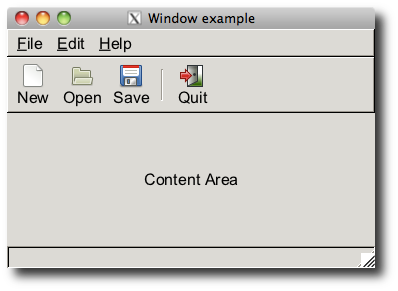
\includegraphics[width=.6\textwidth]{ex-RGtk2-UI}
  \caption{A GUI made using a UI manager to layout the menubar and toolbar.}
  \label{fig:RGtk2-UI}
\end{figure}


We begin by constructing the UI manager:
\begin{Schunk}
\begin{Sinput}
 uimanager = gtkUIManager()
\end{Sinput}
\end{Schunk}

Next, we define the action groups. For demonstration purposes, our
actions simply push the action name onto the status bar at the bottom
of the window:
\begin{Schunk}
\begin{Sinput}
 someAction <- function(action,...) 
   statusbar$push(statusbar$getContextId("message"), 
                  action$getName())
\end{Sinput}
\end{Schunk}
%
We also need a quit handler:
\begin{Schunk}
\begin{Sinput}
 Quit <- function(...) win$destroy()
\end{Sinput}
\end{Schunk}

We break up our action group definitions into one for ``File'',
and ``Edit'' and one for ``Help.'' Every action is defined by a
\class{GtkActionEntry} structure, which is represented by a list in
\R. The components (in order) are the name; the icon; the
label, with \code{\_} specifying the mnemonic; the keyboard
accelerator, with \code{<control>}, \code{<alt>}, \code{<shift>} as
possible prefixes, a tooltip, and finally the callback. Empty values
can be defined as \code{NULL} or, except for the callback, an empty
string.

We define the actions for the ``File'' and ``Edit'' menus:
\begin{Schunk}
\begin{Sinput}
 firstActionGroup <- gtkActionGroup("firstActionGroup")
 firstActionEntries <- list(
   ## name,ID,label,accelerator,tooltip,callback
   file = list("File",NULL,"_File",NULL,NULL,NULL),
   new = list("New", "gtk-new", "_New", "<control>N", 
     "New document", someAction),
   sub = list("Submenu", NULL, "S_ub", NULL, NULL, NULL),
   open = list("Open", "gtk-open", "_Open", "<ctrl>0", 
     "Open document", someAction),
   save = list("Save", "gtk-save", "_Save", "<alt>S", 
     "Save document", someAction),
   quit = list("Quit", "gtk-quit", "_Quit", "<ctrl>Q", 
     "Quit", Quit),
   edit = list("Edit", NULL, "_Edit", NULL, NULL, NULL),
   undo = list("Undo", "gtk-undo", "_Undo", "<ctrl>Z", 
     "Undo change", someAction),
   redo = list("Redo", "gtk-redo", "_Redo", "<ctrl>U", 
     "Redo change", someAction)
 )
\end{Sinput}
\end{Schunk}
%
In the above, we create dummy actions named ``File'' and ``Edit'' that
perform no function. They are necessary for specifying the menu layout
later. We now add the actions to the action group, then add this
action group to the first spot in the UI manager:
\begin{Schunk}
\begin{Sinput}
 firstActionGroup$addActions(firstActionEntries)
 uimanager$insertActionGroup(firstActionGroup, 0) # 0-based
\end{Sinput}
\end{Schunk}

The redo feature should only be sensitive to mouse
events after a user has undone an action. If we wanted to alter the
sensitivity of the redo action, we would need to retrieve it from the
action group:
\begin{Schunk}
\begin{Sinput}
 redo <- firstActionGroup$getAction("Redo")
 redo['sensitive'] <- FALSE
\end{Sinput}
\end{Schunk}

It is also possible to define toggle actions, as we demonstrate
presently for the ``Help'' group. First, we define the ordinary actions:
\begin{Schunk}
\begin{Sinput}
 helpActionGroup <- gtkActionGroup("helpActionGroup")
 helpActionEntries <- list(
   help = list("Help", "", "_Help", "", "", NULL),
   about = list("About", "gtk-about", "_About", "", "", 
     someAction)
 )
 helpActionGroup$addActions(helpActionEntries)
\end{Sinput}
\end{Schunk}
%
Next, we define a ``Use tooltips'' toggle action:
\begin{Schunk}
\begin{Sinput}
 toggleActions <- list(
   tooltips = list("UseTooltips", NULL, "Use _Tooltips", "<control>T", 
     "Enable tooltips", someAction, TRUE)
 )
 helpActionGroup$addToggleActions(toggleActions)
\end{Sinput}
\begin{Soutput}
NULL
\end{Soutput}
\end{Schunk}
%
The list structure for toggle action entry is identical to that of the
ordinary actions, except for the last element which indicates whether
the action is initially active.  One can also incorporate radio
actions, although this is not shown.  Finally, we insert the help
action group in the second position:
\begin{Schunk}
\begin{Sinput}
 uimanager$insertActionGroup(helpActionGroup, 1)
\end{Sinput}
\end{Schunk}
%

Our menubar and toolbar layout is specified as XML according to a
schema specified by the UI manager framework. The XML can be stored in
a file or an \R\/ character vector.  The structure of the file can be
grasped quickly from this example:
\begin{verbatim}
<ui>
  <menubar name="menubar">
    <menu name="FileMenu" action="File">
      <menuitem name="FileNew" action="New"/>
      <menu action="Submenu">
	<menuitem name="FileOpen" action="Open" />
      </menu>
      <menuitem name="FileSave" action="Save"/>
      <separator />
      <menuitem name="FileQuit" action="Quit"/>
    </menu>
    <menu action="Edit">
      <menuitem name="EditUndo" action="Undo" />
      <menuitem name="EditRedo" action="Redo" />
    </menu>
    <menu action="Help">
      <menuitem action="UseTooltips"/>
      <menuitem action="About"/>
    </menu>
  </menubar>
  <toolbar name="toolbar">
    <toolitem action="New"/>
    <toolitem action="Open"/>
    <toolitem action="Save"/>
    <separator />
    <toolitem action="Quit"/>
  </toolbar>
</ui>
\end{verbatim}
% \VerbatimInput{ex-menus.xml}

The top-level element is named \code{ui}, only one of which is allowed
in a UI definition. The children of \code{ui} represent a top-level
action container: \code{menubar}, \code{toolbar}, or \code{popup}.
The \code{name} attributes are used to refer to the widgets later. The
\code{menubar} element contains \code{menu} elements, which in turn
contain \code{menuitem} and \code{separator} elements, as well as
additional \code{menu} elements for nesting. The toolbars are
populated with \code{toolitem} elements. The item elements have an
\code{action} attribute that refers to an action in one of our action
groups and an optional name (defaulting to the \code{action} value).

This file is loaded into the UI manager as follows
\begin{Schunk}
\begin{Sinput}
 id <- uimanager$addUiFromFile("ex-menus.xml")
\end{Sinput}
\end{Schunk}
%
The \code{id} value can be used to merge and delete UI components
according to the mode of the UI, but this is not illustrated here.

Now we can setup a basic window template with a menubar, toolbar, and
status bar. We first construct the three main widgets. The UI manager
will construct our toolbar and menubar, as identified from the names
specified in the UI definition:
\begin{Schunk}
\begin{Sinput}
 menubar <- uimanager$getWidget("/menubar")
 toolbar <- uimanager$getWidget("/toolbar")
\end{Sinput}
\end{Schunk}
The statusbar is constructed with
\begin{Schunk}
\begin{Sinput}
 statusbar <- gtkStatusbar()
\end{Sinput}
\end{Schunk}
%

Now we create a top-level window and attach a keyboard accelerator
group to the window so that when the window has the focus, the
keyboard shortcuts defined for our actions are active:
\begin{Schunk}
\begin{Sinput}
 win <- gtkWindow(show=TRUE)
 win$setTitle("Window example")
 accelgroup <- uimanager$getAccelGroup()
 win$addAccelGroup(accelgroup)
\end{Sinput}
\end{Schunk}

Now it is a simple matter of packing the widgets into a box.
\begin{Schunk}
\begin{Sinput}
 box <- gtkVBox()
 win$add(box)
 box$packStart(menubar, expand=FALSE, fill=FALSE, 0)
 box$packStart(toolbar, expand=FALSE, fill= FALSE, 0)
 contentArea <- gtkVBox()
 box$packStart(contentArea, expand=TRUE, fill=TRUE, 0)
 contentArea$packStart(gtkLabel("Content Area"))
 box$packStart(statusbar, expand=FALSE, fill=FALSE, 0)
\end{Sinput}
\end{Schunk}

\end{example}

%% TODO: this needs to go somewhere.. appendix?
%% \SweaveInput{Classes}


% \label{sec:RGtk2:dialogs}
% \SweaveInput{Pre-defined-dialogs}

% \chapter{\code{cairoDevice}}
% \label{sec:RGtk2-cairoDevice}
% \SweaveInput{cairoDevice}

% \chapter{Using \code{glade} to design GUIs}
% \label{sec:RGtk2-glade}
% \SweaveInput{Glade}

%\section{End of chapter notes}
%\label{sec:RGtk2:end-of-chapter}

% * overview in inst
% * gtk tutorial in R
% * API at http://developer.gimp.org/api/2.0/gtk/
% * ...

% * widget gallery
% http://library.gnome.org/devel/gtk/stable/ch02.html

%  good source: http://developer.gnome.org/doc/GGAD/ggad.html

% * http://gtk.org/documentation.html

% * gtk API
% http://library.gnome.org/devel/gtk/stable/

% * pango manual 
% http://library.gnome.org/devel/pango/stable/PangoMarkupFormat.html

% * Missing discussion on standard dialogs: message, confirmations, etc.
% filebrowser, colors selector, font selector, 

% * Mention history: GIMP; GNOME; DTL RGtk; Michael Lawrence RGtk2
% * Installation: windows; linux; mac OS X

% * Info
% php cookbook good source of info

% DTL examples from omegahat

% pygtk tutorial easier to read than C one (no types specifed)
% pygtk cookbook: http://eccentric.cx/misc/pygtk/wiki/doku.php?id=pygtk
% pygtk faq: http://faq.pygtk.org/index.py?req=index


%% Need a comparison of RGtk2 and qtbase, somewhere (appendix? qt chapter?)

%% High-level comparison of frameworks:

%% Feature     Qt            GTK+           R
%% ------------------------------------------------------------------------
%% DBus        QtDBus        GDBus (GIO)    None (RCorba is Windows Equivalent)
%% XML UI      QtUiTools     GtkBuilder     RGG (Java)  
%% GUI         QtGui         GTK+           tcltk
%% Help        QtHelp        Yelp (Gnome)   R help system (primitive)   
%% Multimedia  QtMultimedia  GStreamer      None
%% IO/Network  QtNetwork     GIO            R connections (synchronous only)
%% OpenGL      QtOpenGL      GlExt/Cairo    rgl
%% Javascript  QtScript      None           None
%% SQL         QtSql         libgda         DBI (good enough)
%% SVG         QtSvg         cairo/librsvg  cairoDevice, svgImport, etc
%% Web browser QtWebkit      GtkWebkit      None     
%% XML         QtXml         libxml         XML (binds libxml)
%% Settings    QtNetwork     GIO            Nothing really

%% Notes:
%% - DBus is likely useless, except on Linux
%% - Deepayan's qtutils package integrates R docs with QtHelp
%% - Multimedia could be useful for generating videos, etc (out of scope)
%% - R connections are very primitive (no asynchronous I/O)
%% - Qt provides 2D API for OpenGL
%% - DBI package covers database access needs
%% - SVG not designed for interactivity, <canvas> better
%% - GtkWebkit should be bound in separate package (worth it?)
%% - XML package has XML handling covered
%% - The graphics support in QtGui is a major advantage over
%%   Cairo-based GTK+. The QPainter API is better designed for stat
%%   graphics and has faster backend implementations. QGraphicsView is
%%   a mature canvas, something GTK+ lacks.

%% Summary: 
%% - Useful features in qtbase, but not RGtk2: WebKit, Multimedia
%%   - GtkWebkit, GStreamer could be bound, but not worth it, given qtbase
%%   - QtWebkit offers Javascript <-> Qt bridge via QtScript

%%%%%%%%%%%%%%%%%%%%%%%%%%%%%%%%%%%%%%%%%%%%%%%%%%


